\graphicspath{{./Sections/Chapter5_instability/figures/}}
\newcommand{\poisson}{\eta} %Poisson's ratio of the channel walls
\newcommand{\aspect}{a} %aspect ratio: \aspect = [z]/[y]
\newcommand{\jump}[1]{_{#1-}^{+}} %jump conditions across interface
\newcommand{\amplitude}{\delta} %amplitude of perturbation in scaling

%dimensionless variables: uncomment below to leave hats on
 \renewcommand{\familydefault}{\sfdefault}

%\newcommand{\h}{\hat{h}}
%\newcommand{\x}{\hat{x}}
%\newcommand{\y}{\hat{y}}
%\newcommand{\that}{\hat{t}}
%\newcommand{\nablahat}{\hat{\nabla}}

\newcommand{\h}{h}
\newcommand{\x}{x}
\newcommand{\y}{y}
\newcommand{\that}{t}
\newcommand{\nablahat}{\nabla}

%for use in the small deformation asymptotics
\newcommand{\X}{X} %for the asymptotics when rescaling with V
\renewcommand{\K}{K} %rescaled wavenumber

\newcommand{\GG}{\psi} %perturbation size after rescaling with nu V^3 (the size of the shear term)
\newcommand{\GGG}{\upsilon} %perturbation pressure rescaling with nu V^3 (the size of the shear term)
\chapter{Bendo-capillary instability of a channel}

In this chapter, we extend the work of the rest of this thesis to consider channels that vary in the third spatial direction.

As motivation, we consider the experiment described in \S 1.4.4 (shown again in Figure~\ref{fig:InstabilityChapter:Intro:ExptSnapshots}(a)). Recall that in these experiments, droplets nucleate at the base of a three-dimensional array of channels and their upper surface moves towards the free end of the channels (the ends closest to the camera, see Figure~\ref{fig:InstabilityChapter:Intro:ExptSnapshots}) in a process reminiscent of bendotaxis. As this takes place, a periodic pattern emerges in the in-plane direction (we refer to variations in the plane parallel to the undeformed channel walls as being `in-plane', and variations in the across channel plane as being `transverse', see Figure~\ref{fig:InstabilityChapter:Intro:ExptSnapshots}(b)). This pattern emerges at relatively early times, and persists throughout the experiment (visible in Figure~\ref{fig:InstabilityChapter:Intro:ExptSnapshots}(a)3--6); its periodicity suggests a preferential wavelength for growth in the transverse direction. We therefore turn now to a first study of this instability.

We focus on three key questions in this chapter: Is the growth of periodic perturbations a generic feature of bendo-capillary systems in which transverse bending and flow are allowed? If so, which physical processes control the wavelength that emerges? And, how does the addition of liquid via condensation mediate this mode selection?


\begin{figure}[h]
\centering
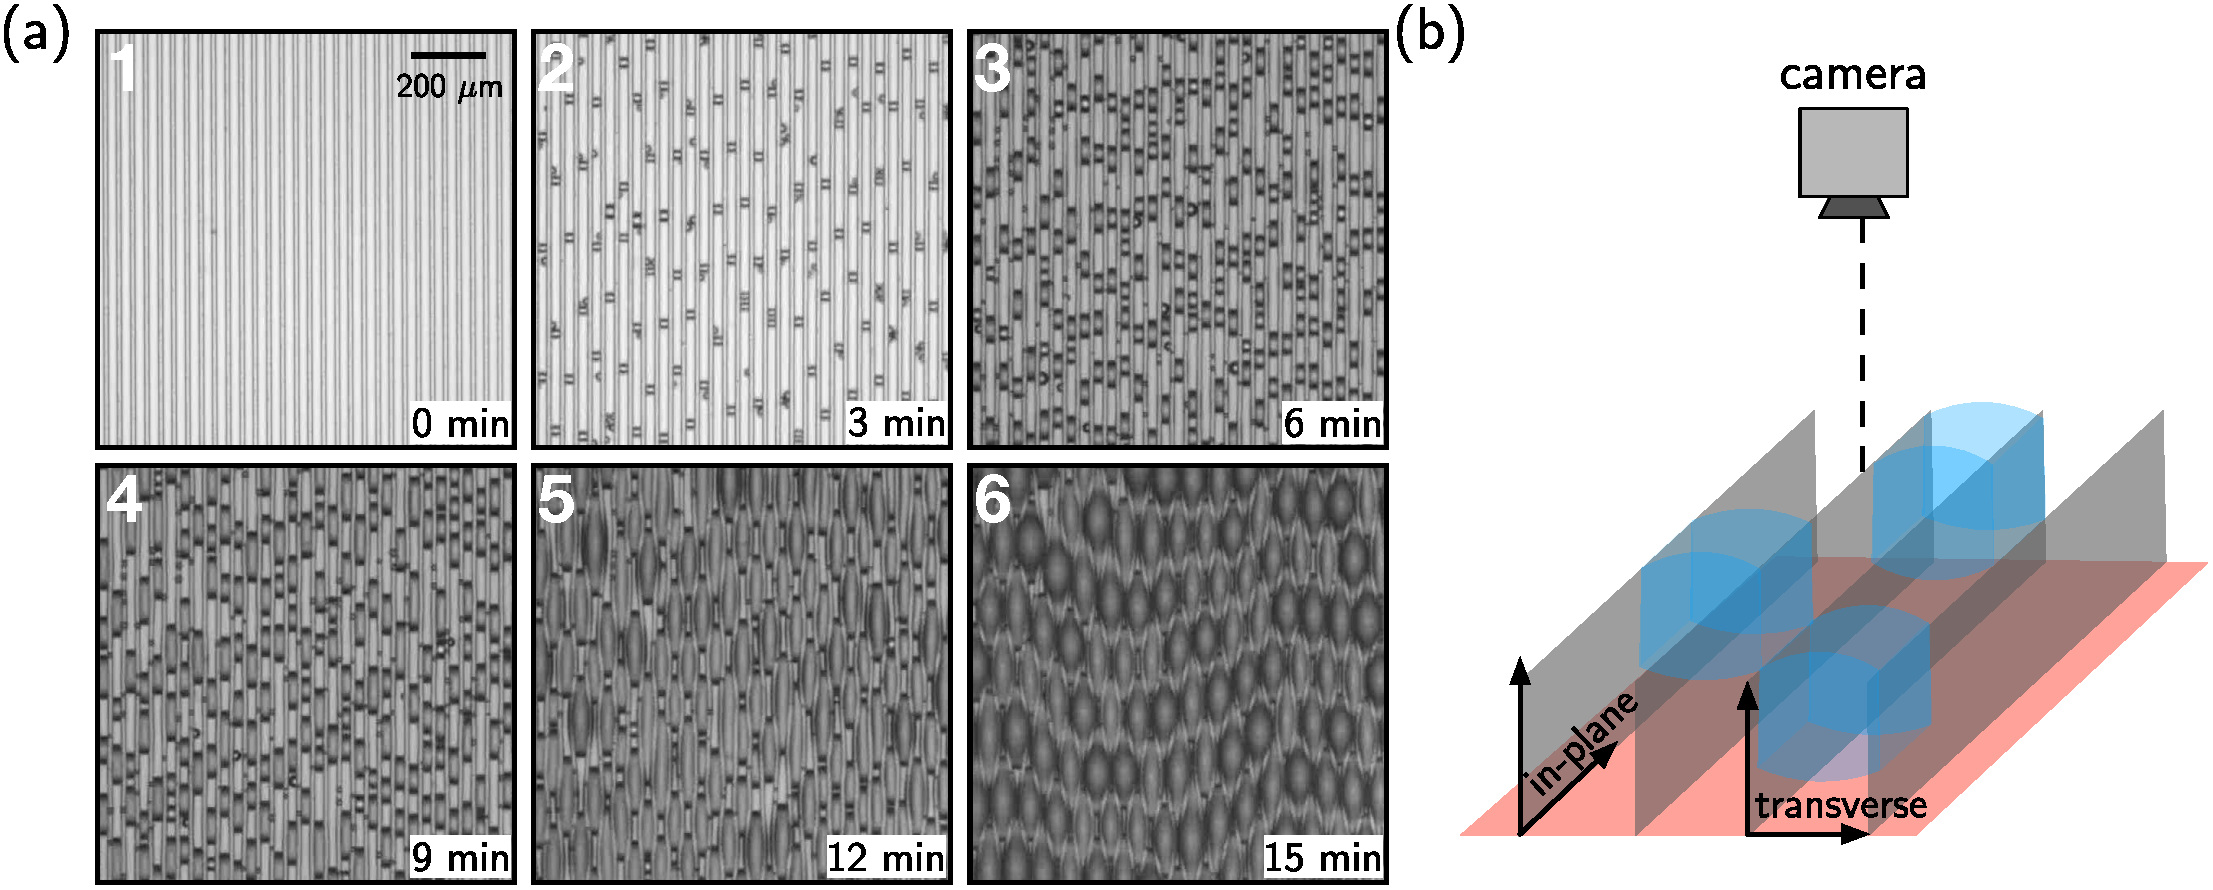
\includegraphics[width = \textwidth]{BrinkmannExperiments}
\caption{(a) Snapshots of experiments performed by~\cite{Seemann2011JPhysCondMat} in which liquid droplets condense within an array of deformable microchannels and eventually reach the free end of the channel. Notice how the emergent periodic pattern appears at relatively early times. (b) Schematic diagram of the experiments shown in (a). We refer to variations in the plane parallel (perpendicular) to the channel walls as in-plane (transverse, respectively), as indicated}
\label{fig:InstabilityChapter:Intro:ExptSnapshots}
\end{figure}

This chapter is structured as follows. In the first section, we describe (our hypothesis for) the mechanism driving the `weaving' instability responsible for the pattern formation, and then gain physical insight via a scaling argument. In the third section, we develop a mathematical model for a simple bendo-capillary system which may be susceptible to the instability. The remainder of the chapter is dedicated to  studying the mode selection process; initially we focus on the case when the liquid volume is constant, before considering the effect of adding liquid volume via condensation.


\section{Mechanism}
We hypothesize that the periodic pattern seen in Figure~\ref{fig:InstabilityChapter:Intro:ExptSnapshots} is the result of an instability, with the observed wavenumber of instability determined as that of the fastest growing mode. In this chapter, we investigate the possibility that this preferred mode is determined by a competition between interfacial curvatures in the transverse and in-plane directions (which we refer to as a `competing-curvature' instability).

\subsection{Competing curvature instabilities: Rayleigh-Plateau}

%how does perturbation change curvatures
The canonical example of a competing-curvature instability is the Rayleigh-Plateau instability~\citep{Plateau1873, Rayleigh1879PRSL, Rayleigh1892PhilosMag}: in the absence of gravity, a thin thread of liquid of uniform radius $r$  may remain in equilibrium (Figure~\ref{fig:InstabilityChapter:Mechanism:Mechanism}(a)) since the constant pressure this requires is consistent with the constant pressure difference across a meniscus of constant curvature.
If the interface is disturbed slightly by an axisymmetric perturbation, periodic in the in-plane direction the transverse curvature -- inversely proportional to the local radius of the thread -- increases (decreases) at troughs of lower radius (peaks of higher radius, respectively). The opposite is true of the in-plane curvature, which is negative at (locally) concave troughs and positive at convex peaks (Figure~\ref{fig:InstabilityChapter:Mechanism:Mechanism}(a)). The difference in the in-plane curvature between peaks and troughs increases from zero with the wavenumber, while the difference in the transverse curvature is independent of it.  As a result, perturbations with sufficiently small wavenumbers (specifically $k < 1/r$) result in a decrease (increase) in the total curvature -- and hence pressure -- at peaks (troughs, respectively), resulting in liquid being driven from troughs to peaks and thus amplifying the perturbation.

\begin{figure}[t]
\centering
\includegraphics[width = \textwidth]{mechanism_png_subfigs}
\caption{Air-liquid interfaces in competing-curvature instabilities. (a)(Left) A thread of liquid with radius $r$ has interfacial curvatures $\kappa_{\parallel}$ and $\kappa_{\perp}$ in the in-plane and transverse directions, respectively (the schematic diagram indicates the orientation of the planes).  (Right) The pressure differences associated with the variable curvatures following a perturbation drives fluid from high to low transverse curvature, leading to the Rayleigh-Plateau instability. (b)-(d) Schematic diagrams of the interface between liquid and air in a narrow channel. The interface has curvature components $C_{\perp}$ and $C_{\parallel}$ (taken in the same planes as in (a)). The base state (b) has no in-plane curvature. The effect of perturbing the interface from the base state differs between (c) rigid, tapered and (d) flexible channels. Arrows indicate the local curvature changes, relative to the base state.}
\label{fig:InstabilityChapter:Mechanism:Mechanism}
\end{figure}


\subsection{The Effect of confinement: Al-Housseiny}
If the liquid is confined between two plates with a gap thickness that varies in the transverse direction (Figure~\ref{fig:InstabilityChapter:Mechanism:Mechanism}(b),(c)), a competing curvature instability is also possible.  (Note that confinement can alter mode selection in the Rayleigh-Plateau instability if the liquid does not contact the walls but is surrounded by a second liquid~\citep{Son2003Macromolecules}, but we do not consider this scenario here.) In the confined case, the stable configuration is a uniform advancing front with no in-plane curvature, $C_{\parallel} = 0$. The key difference between this scenario and the free interface is that here the confinement sets the transverse curvature; the total curvature of the base state is  $C(x) = C_{\parallel}  + C_{\perp} =  C_{\perp} = -2 \cos \theta/h(x)$~\citep{deGennes2004}, where $h(x)$ is the (non-constant) channel thickness, $\theta$ is the contact angle between the liquid and the plates, and the $x$-axis is aligned along the channel  (Figure~\ref{fig:InstabilityChapter:Mechanism:Mechanism}(b)).

Consider first a wetting configuration, $\theta < 90$\si{\degree}. Provided the channel is narrowing, a periodic perturbation to the interface (Figure~\ref{fig:InstabilityChapter:Mechanism:Mechanism}(c)) decreases the channel width at protrusions (where the liquid advances ahead of the original meniscus position) and thus increases the magnitude of the transverse curvature  $C_{\perp}$ there (corresponding to a more negative capillary pressure). Invaginations experience a decrease in the magnitude of the transverse curvature, and hence a reduction in the suction pressure, owing to the weaker confinement. As a result, protrusions may suck liquid from invaginations, thus increasing the size of the perturbation and destabilizing the interface.

As in the Rayleigh-Plateau instability, the transverse curvature changes are in competition with the in-plane curvature $C_{\parallel}$, which offers a stabilizing effect whose strength increases with wavenumber. Again, perturbations of a sufficiently small wavenumber are amplified (the range of unstable wavenumbers depends on the contact angle, and the local channel thickness and tapering angle). This scenario has been studied in detail (both theoretically and experimentally) in recent years~\cite[see][for example]{Protiere2010EPL, AlHousseiny2012NaturePhysics,AlHousseiny2013PhysFlu,Keiser2016JFM, LedesmaAguilar2017SoftMatter}.

If the liquid does not wet the channel ($\theta> 90\si{\degree}$), protrusions (invaginations) of a perturbation to the meniscus experience a decrease (increase, respectively) in transverse curvature, provided the channel is widening; the convex interface experiences a weaker (stronger) confinement. Again, perturbations of sufficiently small wavenumber will be amplified. We stress that this instability is only possible for non-wetting configurations if the channel is widening (in the direction of advancing interface) and only possible for wetting configurations if the channel is narrowing.

%I don't think I need to mention confined RP instability (e.g. Tomotika, 1935 and Son, 2003): they're not looking at contact.

\subsection{Introducing elasticity}\label{S:InstabilityChapter:Mechanism:Elasticity}
If the tapered wall is not rigid but deforms in response to liquid pressure (Figure~\ref{fig:InstabilityChapter:Mechanism:Mechanism}(d)), the picture changes in two important ways. Firstly, the global tapering of the channel is set by the bulk liquid pressure. With the familiar clamped-free conditions on the beams, the induced tapering will always be in the direction that favours instability: wetting configurations will be tapered inwards, and non-wetting configurations will be tapered outwards. This means that, unlike the rigid case, it is possible that both wetting and non-wetting configurations will be susceptible to the bendo-capillary competing curvature instability within the same channel.

The second important difference with the competing curvature instability in a rigid confinement it that a meniscus perturbation will result in an additional elastic response from the channel. Protrusions will apply a pressure over a longer portion of the channel, compared to the flat base state, resulting in an enhanced wall response; the confinement that a protrusion experiences will be exacerbated (and the confinement an invagination experiences will be reduced) by the elastic response to the perturbation. This, in turn, will lead to a greater difference in the destabilizing transverse curvature between meniscus protrusions and invaginations. We anticipate that this may extend the range of unstable modes, or make the growth rate faster, than the corresponding rigid case.


\section{Scaling argument}\label{S:InstabilityChapter:Scaling}

Before developing a detailed model, we seek first to gain some quantitative insight into mode selection driven by the mechanism described in \S\ref{S:InstabilityChapter:Mechanism:Elasticity}. We consider the configuration shown in Figure~\ref{fig:InstabilityChapter:SlowCondensation:Scaling:ToyProblem}: a section of a channel with width $\lambda$ and length $L$ contains liquid sat at a rigid base of thickness $2H$, while the opposite end is open. The other two walls of the channel are narrow and flexible; they bend in response to the liquid pressure (characterized by a bending stiffness $B$), but for simplicity we allow them to bend only along their length (i.e.~in the transverse direction). They are clamped at the rigid base. We imagine a cut along the centre of each deformable wall (black dashed lines in Figure~\ref{fig:InstabilityChapter:SlowCondensation:Scaling:ToyProblem}), so that the two halves can deform independently of one another. In effect, we allow liquid to flow between the two halves of the (section of) channel, whilst neglecting in-plane bending. (Any instability that appears in this system will be a discrete square wave instability.)

\begin{figure}[t]
\centering
\includegraphics[width = \textwidth]{Scaling_3d}
\caption{Schematic diagrams of section of a flexible channel consisting of a solid base and two flexible walls, which are only permitted to bend along their length. A cut along each of the flexible walls (black dashed line) allows the two halves to bend independently. (a) The system is in equilibrium with the meniscus located a distance $x_m$ from the base.  (b) The equilibrium is perturbed by moving the menisci on either side of the cut a distance $\delta$; if $\lambda$ is sufficiently large, this perturbation results in the flow of liquid from troughs (blue) to peaks (red) with speed $U$, amplifying the perturbation, as described in the main text.}
\label{fig:InstabilityChapter:SlowCondensation:Scaling:ToyProblem}
\end{figure}

For the moment, we assume that the fraction of the channel occupied by liquid is relatively small. (This is the situation at early times in the condensation experiments that motivate this work; pattern formation first occurs in these early stages.) In this simple argument, we assume that no condensation occurs in the time interval of interest: the amount of liquid in the channel remains constant.

To make the analysis presented in this chapter more tractable, we consider the situation in which the condensed liquid remains in contact with the base. In this case, a two-dimensional equilibrium exists~\citep{Taroni2012JFM}.

Consider such an equilibrium configuration in which the meniscus is located a distance $x_m$ from the clamped base. As the volume of liquid is relatively small, the walls are not deformed significantly and the channel half-width at the meniscus $h_m \sim H$ (see Figure~\ref{fig:InstabilityChapter:SlowCondensation:Scaling:ToyProblem}(a)). By conservation of mass, the meniscus position is $x_m \sim \Omega / H$, where $\Omega$ is the cross sectional volume. The liquid pressure in this configuration is $p_m \sim -\gamma \cos \theta/H$, where $\gamma$ is the surface tension coefficient of the liquid, and $\theta$ the contact angle between the liquid and channel wall.

Before we consider perturbations to this equilibrium, we need a scaling for $h_m'$, the channel slope at the meniscus. By considering a cantilever beam with bending stiffness $B$ bending over a length scale $x_m$ by a uniform (Laplace) pressure $-\gamma \cos \theta / H$ we find~\citep{Timoshenko1959},
\begin{equation}\label{E:InstabilityChapter:Scaling:hmprimed}
h_m' \sim -\frac{\gamma \cos \theta x_m^3}{B H}.
\end{equation}

We mimic a periodic perturbation of wavenumber $k = 2\pi/\lambda$, and amplitude $\amplitude$, by considering a region of length $\lambda$, with each split region having length $\lambda/2$ (as in f
Figure~\ref{fig:InstabilityChapter:SlowCondensation:Scaling:ToyProblem}). We then force one side of the cut to advance (uniformly) to $x_0 + \amplitude$ and the other to retreat to $x_0 - \amplitude$ (Figure~\ref{fig:InstabilityChapter:SlowCondensation:Scaling:ToyProblem}(b)). As discussed, the transverse interfacial curvature, and thus liquid pressure, changes as a result of this perturbation: the transverse curvature changes as the interface is forced into a stronger (or weaker) confinement and, additionally, the confinement responds to the perturbation as the liquid pressure is now applied over a different length of the channel walls. With this `discrete' perturbation, there is no stabilizing surface tension term, which would usually come from the in-plane curvature. Here, we put this in manually by adding a pressure penalty $\gamma \delta k^2$ to the pressure in the protruding half.

\subsection{Mode selection}
The perturbation will grow when the difference in liquid pressure between the two halves, $\Delta P = p_+ - p_-$, drives liquid towards the protruding half (the red half in Figure~\ref{fig:InstabilityChapter:SlowCondensation:Scaling:ToyProblem}), i.e.~when $\Delta P<0$.

To leading order in $\amplitude$, we find that
\begin{equation}\label{E:InstabilityChapter:Scaling:DeltaP_preliminary}
\Delta P\sim \gamma\left(\frac{\cos \theta}{h_-} - \frac{ \cos \theta}{h_+} + \beta \amplitude k^2\right) \sim \gamma \left(\frac{\Delta h \cos \theta}{h_m^2} + \beta \amplitude k^2\right),
\end{equation}
where $\beta>0$ is an $\mathcal{O}(1)$ scaling constant and $\Delta h = h_+ - h_- $ is the difference in the channel widths at the menisci between the two halves (see Figure~\ref{fig:InstabilityChapter:SlowCondensation:Scaling:ToyProblem}(b)).

To find a scaling for $\Delta h$, we decompose it into a contribution from the meniscus advancing/receding into a tapered channel, and a contribution from the elastic response to the perturbation:
\begin{equation}\label{E:InstabilityChapter:Scaling:ChangeInH}
\Delta h = \Delta h_\text{tapering} + \Delta h_\text{elastic}.
\end{equation}

To leading order in $\amplitude$, the tapering contribution has the same scaling as a meniscus advancing into a rigid channel, whose angle is set by the equilibrium configuration, i.e.
\begin{equation}\label{E:InstabilityChapter:Scaling:ChangeInHtapering}
\Delta h_\text{tapering} \sim \amplitude h_m' \sim -\delta \frac{\gamma  \cos \theta x_0^3}{B H},
\end{equation}
where we have used the scaling~\eqref{E:InstabilityChapter:Scaling:hmprimed} for $h_m'$.

The leading order elastic contribution is found by considering a cantilever beam of length $x_m$ loaded with the equilibrium liquid pressure $p_0 = -\gamma \cos \theta/H$ (the dry region of the beam offers no resistance to bending in this scenario). If the length of the beam increases in length to $x_m + \delta$, the corresponding increase in deflection of its tip is
\begin{equation}\label{E:InstabilityChapter:Scaling:ChangeInHelastic}
\Delta h_\text{elastic} \sim -\frac{p_0}{B}\left[ \left(x_m + \amplitude\right)^4 - x_m^4\right] \sim  -\amplitude \frac{\gamma \cos \theta x_m^3}{BH}.
\end{equation}

Perhaps surprisingly, both the elastic and tapering contributions to $\Delta h$ have the same scaling but, in any case, substituting this in to~\eqref{E:InstabilityChapter:Scaling:DeltaP_preliminary} gives
\begin{equation}\label{E:InstabilityChapter:Scaling:DeltaP}
\Delta P \sim -\delta \gamma \left(\frac{\gamma \cos^2 \theta}{H^2}\frac{ x_m^3}{B H} - \beta k^2\right).
\end{equation}

By balancing the terms in~\eqref{E:InstabilityChapter:Scaling:DeltaP}, we obtain
a scaling for the wavenumber of unstable modes:
\begin{equation}\label{E:InstabilityChapter:Scaling:CriticalWavenumber}
k_c \sim  \left(\frac{\gamma \cos^2 \theta x_m^3}{B H^3}\right)^{1/2}
\end{equation}
We expect that perturbations with wavenumber $k \lesssim k_c$ will be unstable, while those will wavenumber $k \gtrsim k_c$ will be damped. This prediction is independent of the wettability: both wetting and non-wetting configurations of sufficiently small wavenumber may be amplified, as we suggested in \S\ref{S:InstabilityChapter:Mechanism:Elasticity} when first describing the mechanism.

\subsection{Growth rates}
When $\Delta P < 0$, liquid is sucked from the invaginations into protrusions with a typical velocity $U$ (Figure~\ref{fig:InstabilityChapter:SlowCondensation:Scaling:ToyProblem}(b)). To estimate this velocity scale, note that this  pressure difference acts over a length scale $\lambda = 2\pi/k$ and so lubrication theory~\citep{Leal2007} suggests that (provided $\lambda,L \gg H$)
\begin{equation}
U \sim -\frac{H^2}{\mu}\frac{\Delta P}{\lambda}\sim \frac{H^2 \delta \gamma k}{\mu}\left(\frac{\gamma \cos^2 \theta}{H^2}\frac{x_m^3}{B H} - \beta k^2\right).
\end{equation}
The corresponding flux of liquid between the two halves of the channel is
\begin{equation}\label{E:InstabilityChapter:Scaling:Flux}
Q \sim \Omega U \sim \delta \frac{\Omega H^2 k}{\mu}\left(\frac{\gamma \cos^2 \theta}{H^2}\frac{ x_m^3}{B H} - \beta k^2\right),
\end{equation}
and conservation of mass for either section requires
\begin{equation}\label{E:InstabilityChapter:Scaling:MassCons}
H \lambda \dd{\delta}{t} \sim Q.
\end{equation}
Combining~\eqref{E:InstabilityChapter:Scaling:Flux} and~\eqref{E:InstabilityChapter:Scaling:MassCons} gives a scaling for $\sigma$, the growth rate of perturbations, as
\begin{equation}\label{E:InstabilityChapter:Scaling:amplitude_ode}
\sigma = \frac{1}{\delta} \dd{\delta}{t} \sim \frac{\Omega H}{\mu}\left(\frac{\gamma \cos^2 \theta}{H^2}\frac{x_m^3}{B H} - \beta k^2\right)k^2.
\end{equation}

The wavenumber of the fastest growing modes can then be easily shown to scale as $k \sim k_c$, with $k_c$ as given in~\eqref{E:InstabilityChapter:Scaling:CriticalWavenumber}. The corresponding growth rate of the perturbation with this wavenumber is
\begin{equation}\label{E:InstabilityChapter:Scaling:SigmaScaling1}
\sigma_c =  \frac{1}{\delta} \dd{\delta}{t} \sim \frac{\Omega Hk_c^2}{\mu}\left(\frac{\gamma \cos^2 \theta}{H_0^2}\frac{x_m^3}{B H} - \beta k_c^2\right) \sim \frac{\gamma^2 \cos^2 \theta x_m^7}{\mu B H^{4}},
\end{equation}
where the final scaling uses the small deformation scaling $\Omega \sim x_m H$.

While the above calculation is very rough, it suggests that that the growth rate of unstable modes has a sensitive dependence on the amount of liquid in the channel (via the meniscus position $x_m$); as we shall see, this is important when the amount of liquid in the channel is evolving via condensation. We turn now to a more formal calculation but shall refer back to these results.


\section{Mathematical model}
%configuration description: channel
In this section, we develop a formal mathematical model of the system discussed in \S\ref{S:InstabilityChapter:Scaling}. The configuration is shown in Figure~\ref{fig:InstabilityChapter:Modelling:Schematic}(a): a narrow cell of thickness $H$ and length $L$ extends infinitely in the third direction. The channel has a rigid boundary at one end (the $x = 0$ plane), and is free at $x = L$. The other two walls are thin and flexible and, without deformation, coincide with the planes $z = \pm H$; the channel walls are characterized by their thickness $b$, Young's Modulus $E$, density $\rho_s$, and Poisson's ratio $\poisson$. The channel walls have bending stiffness $B = Eb^3 / (12(1-\poisson^2))$~\citep{Timoshenko1959} (We take $\eta = 0.5$, corresponding to incompressible walls, throughout this chapter.)

%configuration description: liquid
 Liquid of viscosity $\mu$, density $\rho_l$ and surface tension $\gamma$ condenses into the channel, and sits at the solid base. We assume the liquid makes a (constant) contact angle $\theta$ with the channel walls. The liquid pressure induces a deformation of the channel walls; in the following sections we describe models for the flow of liquid and deformation of the channel walls and study the coupling between the two.

\begin{figure}[t]
\centering
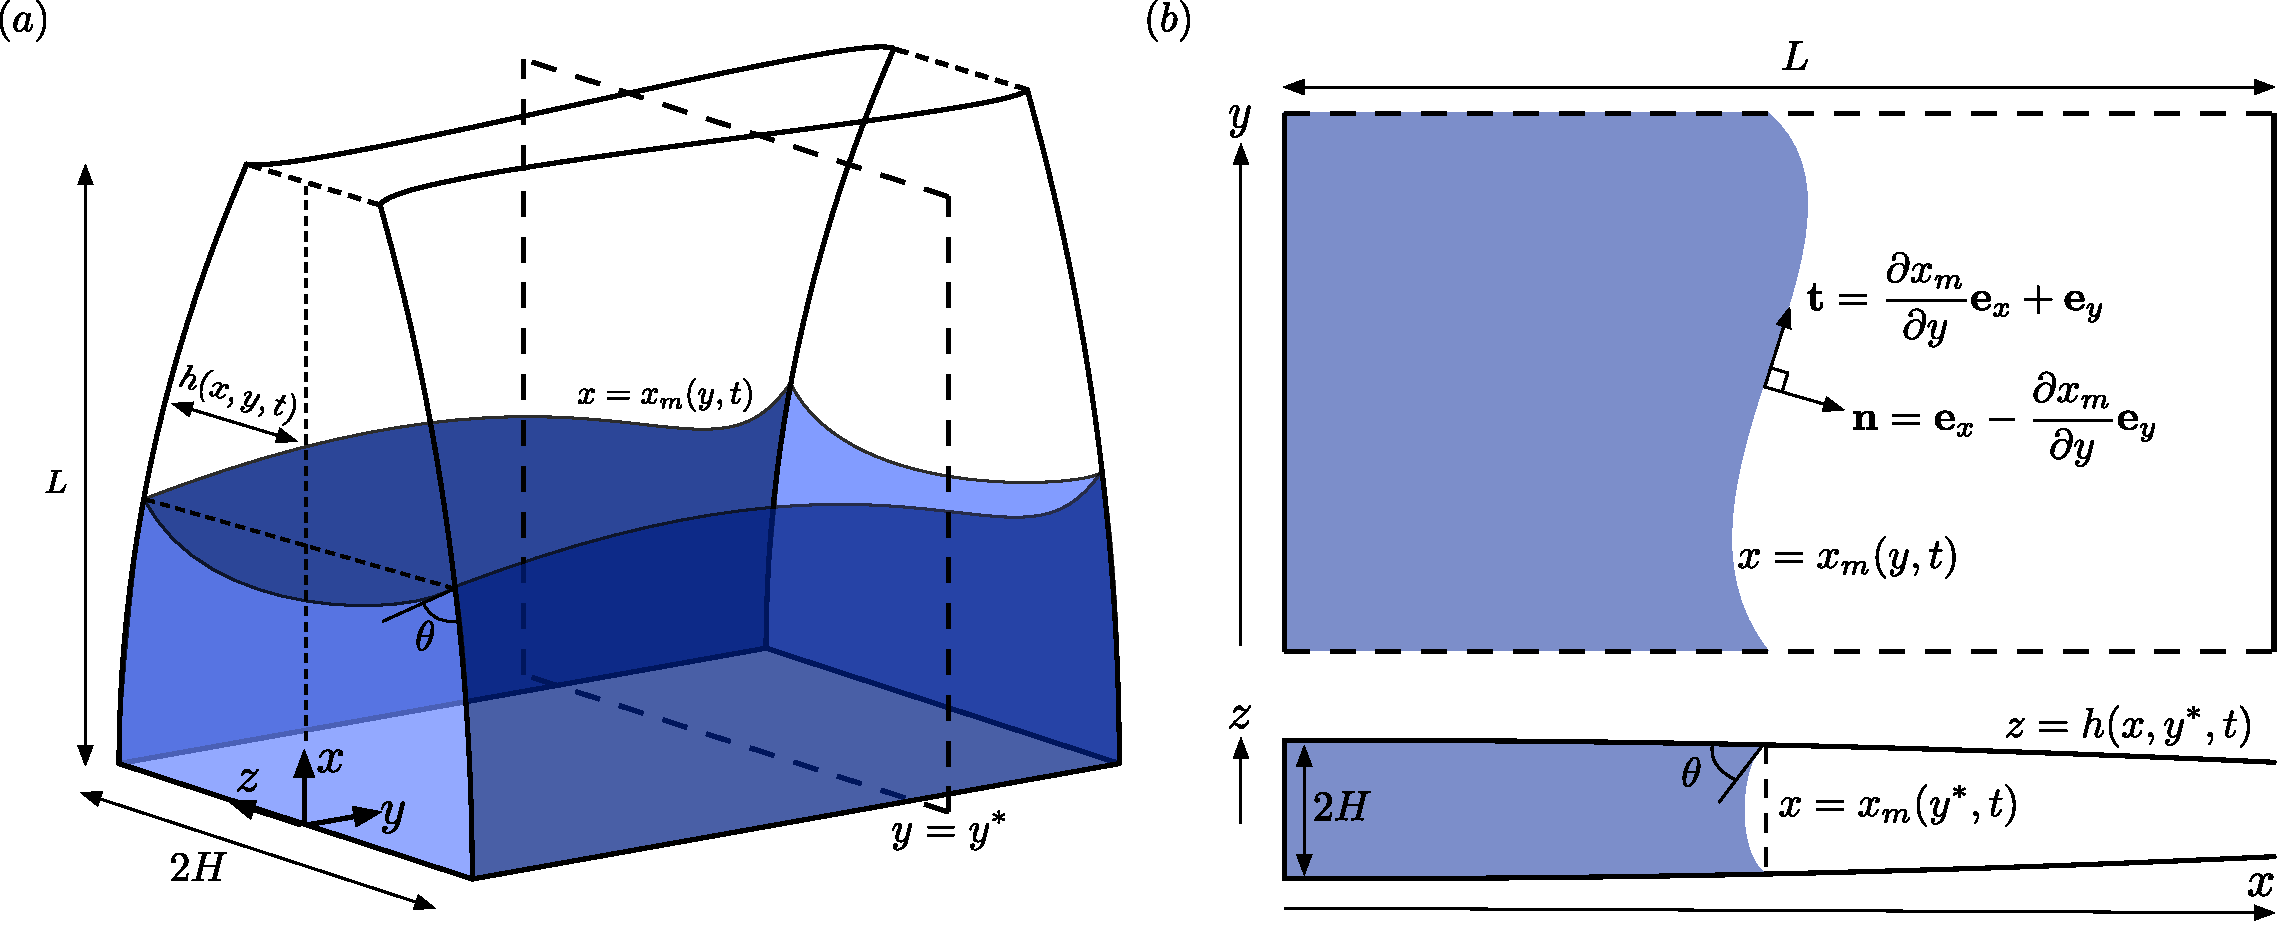
\includegraphics[scale=0.39]{Schematic_two_cross_sections}
\caption{(a) Schematic diagram of liquid in a narrow channel consisting of a solid base at $x =0$ and two deformable walls, whose midplanes are located at $z = \pm h(x,y,t)$. The liquid makes contact with the channel walls at $x = x_m(y,t)$. Note that the cell extends infinitely in the $y$-direction (only a section of which is shown). (b) Cross sections of the system shown in (a) in the $(x,y)$ plane (upper) and $(x,z)$ plane (lower); the latter is taken through $y = y^*$, indicated by the dashed box in (a).}
\label{fig:InstabilityChapter:Modelling:Schematic}
\end{figure}

\subsection{Preliminaries and assumptions}
We assume that the configuration is symmetric about $z = 0$ -- so we only need to consider a single channel wall -- and also that the walls are thin in comparison with their length, $b \ll L$. As a result, we can characterize the channel width at time $t > 0$ entirely by the position of the mid-plane of one wall~\citep{Reddy2006}, denoted by $h(x,y,t)$, (we shall therefore use `wall' and `wall mid-plane' interchangeably).
%We also assume that the channel walls are thin in comparison with the channel half-width, $b \ll H$, so it is reasonable to consider $2h(x,y,t)$ to be the width of the cavity between the walls.

The channel is wetted over a region $0 < x < x_m(y,t)$. We assume that $x_m \gg H$ throughout and also that variations in the flow in the $y$ direction occur on a length scale much longer than $H$, allowing us to use lubrication theory to model the liquid flow. The channel geometry does not provide a natural length scale for variations in the $y$-direction (as it does for the $x$-direction), but the length scale $L$ that we use in the horizontal direction is a natural choice. To ensure the lubrication approximation holds, we must ensure that the typical length scale of flow in the $y$-direction is much longer than $H$, but we shall check this a posteriori. With this assumption, the contact angle between liquid and solid is approximately that measured in the $(x,z)$ plane (Figure~\ref{fig:InstabilityChapter:Modelling:Schematic}(b)).

As in previous chapters, we neglect the weight and inertia of both the liquid and the channel walls, and the line force associated with surface tension.

%%%%%%%%%% Deleted Table %%%%%%%%%
%\renewcommand{\arraystretch}{1.2}
%\begin{table}[t]
%\begin{center}
%\begin{tabular}{ p{4cm} | p{3.5cm} | p{3cm}| p{2.5cm} }
%Neglected physics & In comparison with & Dimensionless no. & Value \\ \hline
%Droplet weight & Capillary forces & Bo = $\rho_l g H^2/\gamma$ & $10^{-5}$ \\
%Wall weight & Capillary forces & $\rho_s b g H/ \gamma$ & $10^{-3}$ \\
%Line force (surface tension) & Laplace Pressure & $\aspect = H/L$ & $10^{-4}$\\
%Droplet inertia & Viscosity & Re =  $\rho_l u_{\text{cap}} L/\mu$ & $10^{-2}$\\
%Wall inertia & Capillary forces & $\sqrt{\rho b L^3\gamma}/(\mu L)$ & $10^{-2}$\\
%Wall stretching & Wall bending & $b/L$ & $10^{-2}$
%\end{tabular}
%\end{center}

%\caption{\textcolor{red}{To be updated}NB: $u_{\text{cap}}$ is the capillary timescale from previous sections, $\mathcal{O}(10\mathrm{s})$. Beam inertia and capillarity calculations from comparing the timescale from beam inertia $T_{i} = \sqrt{IH_0/L^2 |\gamma \cos \theta|}$ and the capillary timescale of the flow $T_c = \mu L^2/ |\gamma \cos \theta|H_0$. $\sqrt{\rho b L^3\gamma}/(\mu L)\sim 10^{-3}$ using experimental values from chapter 3.  }\label{Table:Assumptions}
%\caption{Physical effects neglected in the mathematical model. Values in the final column are order of magnitude estimates from the experiments described in Chapter 3. Here, $u_{\text{cap}} = \gamma H/\mu L$ is the capillary velocity scale.}\label{Table:InstabilityChapter:Modelling:Assumptions}
%\end{table}
%%%%%%%%%% Deleted Table %%%%%%%%%



\subsection{Liquid flow}
Given the assumed small aspect ratio of the flow, we describe it using lubrication theory. The evolution of the pressure field $p(x,y,t)$ and the gap width are then coupled via Reynolds' equation
\begin{equation}\label{E:InstabilityChapter:Model:Liquid:Reynolds}
\ddp{h}{t} = \nabla.\left( \frac{h^3}{3\mu} \nabla p\right) \qquad \text{in}~0 < x < x_m(y,t).
\end{equation}

The free boundary of the liquid moves in response to the flux of fluid there and condensation of liquid onto it. Assuming that liquid condenses onto the interface at a uniform rate $C$ per unit area, the location of the interface evolves according to
\begin{equation}
\ddp{x_m}{t} = -\left.\frac{h^2}{3\mu}\nabla p .\frac{\mathbf{n}}{|\mathbf{n}|}\right|_{x = x_m(y,t)} + C
\end{equation}
where $\mathbf{n} = \mathbf{e}_x -\frac{\partial x_m}{\partial y}  \mathbf{e}_y$ is the normal to the interface in a plane at constant $z$ (Figure~\ref{fig:InstabilityChapter:Modelling:Schematic}(b)).

According to Laplace's law, the liquid pressure immediately beneath the interface is
\begin{equation}\label{E:InstabilityChapter:Model:Liquid:LaplaceBC}
 p(x = x_m, y,t) = \gamma\left(C_{\perp} + C_{\parallel}\right)
\end{equation}
where $C_{\perp}$ and $C_{\parallel}$ are the transverse and in-plane interfacial curvatures, respectively. Our neglect of gravity ensures that the meniscus is locally a circular arc in the $(x,z)$ plane (Figure~\ref{fig:InstabilityChapter:Modelling:Schematic}(b)), and hence
\begin{equation}\label{E:InstabilityChapter:Model:Liquid:CPerp}
C_{\perp} = -\frac{\cos \theta}{h(x=x_m,y,t)}.
\end{equation}

Our assumption that variations in the $y$-direction occur on a length scale much larger than $H$ means that we can approximate the in-plane interfacial curvature by
\begin{equation}\label{E:InstabilityChapter:Model:Liquid:CParallel}
C_{\parallel} = -\ddp{^2 x_m}{y^2}.
\end{equation}

We impose a no-flux condition at the rigid base,
\begin{equation}\label{E:InstabilityChapter:Model:Liquid:nofluxBC}
\ddp{p}{x}=0 \qquad \text{at}~x =0.
\end{equation}

\subsection{Wall deformation}
In the experiments shown in  Figure~\ref{fig:InstabilityChapter:Intro:ExptSnapshots}, the channel walls appear to undergo deformations that are large in comparison with their thickness.  We might expect, therefore, that the modelling of the channel's response to liquid pressure should include self-induced in-plane stretching~\citep{Timoshenko1959}. However, the energy penalty associated with in-plane stretching, which scales with $b/L$, is very high in comparison with the bending energy $(b/L)^3$ for thin flexible objects~\citep{Pini2016SciRep}. We therefore ignore stretching, and the channel walls can therefore be modelled as thin plates undergoing pure bending deformations under an applied load $q(x,y,t)$. The position of the channel wall mid-plane $h(x,y,t)$ therefore satisfies~\citep{Timoshenko1959}
\begin{equation}\label{E:InstabilityChapter:Model:Wall:Bilaplacian}
B\nabla^4 h = q.
\end{equation}

The channel deformation is coupled to the liquid pressure via the applied load:
\begin{equation}\label{E:InstabilityChapter:Model:Wall:BilaplacianPressure}
q(x,y,t) = \left\{\begin{array}{ll}  p(x,y,t) & 0 < x< x_m,\\ 0 & x_m < x < L
\end{array}\right.
\end{equation}

To close the problem, we require boundary conditions at the channel ends, $x= 0$ and $x = L$, as well as at the interface, $x = x_m$. We apply a straightforward clamped condition at $x = 0$,
\begin{equation}\label{E:InstabilityChapter:Model:Wall:ClampedBC}
h= H, \quad \ddp{h}{x} = 0 \qquad \text{at}~x = 0.
\end{equation}
The other boundary conditions require care, as they concern moments and shear forces. The wall supports bending moments
\begin{equation}\label{E:InstabilityChapter:Model:Wall:WallBendingMoments}
M_x = -B\left(\ddp{^2 h}{x^2} + \poisson \ddp{^2 h}{y^2}\right) \quad \text{and}\quad M_y = -B\left(\ddp{^2 h}{y^2} + \poisson \ddp{^2 h}{x^2}\right)
\end{equation}
parallel to the $x$- and $y$-axes, respectively, as well as a twisting moment
\begin{equation}\label{E:InstabilityChapter:Model:Wall:WallTwistingMoments}
M_{xy} = B(1-\poisson)\ddp{^2 h}{x \partial y}.
\end{equation}
Similarly, shear deformation can be decomposed into components $Q_x$ and $Q_y$ in directions parallel to the $x$- and $y$-axes, respectively. These are related to the channel wall position by
\begin{align}
Q_x &=  \ddp{M_x}{x} -\ddp{M_{xy}}{y} = -B \ddp{}{x} \left(\ddp{^2 h}{x^2} +\ddp{^2 h}{y^2}\right),\label{E:InstabilityChapter:Model:Wall:ShearX}\\
Q_y &= \ddp{M_{y}}{y} - \ddp{M_{xy}}{x} = -B \ddp{}{y} \left(\ddp{^2 h}{x^2} + \ddp{^2 h}{y^2}\right).\label{E:InstabilityChapter:Model:Wall:ShearY}
\end{align}
(See~\cite{Timoshenko1959}, for example, for a derivation of~\eqref{E:InstabilityChapter:Model:Wall:WallBendingMoments}--\eqref{E:InstabilityChapter:Model:Wall:ShearY}.)

We apply a free boundary condition at $x = L$:
\begin{equation}\label{E:InstabilityChapter:Model:Wall:FreeEndBC_all}
M_x = 0 = M_{xy} = Q_x \quad \text{at}~x = L.
\end{equation}
For a thin plate undergoing purely bending deformations, however, the three boundary conditions~\eqref{E:InstabilityChapter:Model:Wall:FreeEndBC_all} are too many, and were demonstrated by~\cite{Tait1883} to be equivalent to the two boundary conditions~\citep{Timoshenko1959},
\begin{equation}\label{E:InstabilityChapter:Model:Wall:FreeEndBC}
\ddp{^2 h}{x^2} + \poisson \ddp{^2 h}{y^2} = 0 = \ddp{^3 h}{x^3} + (2-\poisson) \ddp{^3 h}{x \partial y^2}\quad \text{at}~x = L.
\end{equation}
%\red{Does this need more explanation? (p84 of Plates and Shells)}

%Comment on the presence of y derivatives meaning we can't integrate out the dry region, in general?
The free boundary condition~\eqref{E:InstabilityChapter:Model:Wall:FreeEndBC} applies only when the channel walls do not touch. If deformations become large enough for contact,~\eqref{E:InstabilityChapter:Model:Wall:FreeEndBC} must be modified but here we focus on early times when only a small amount of liquid is present and the associated deformations are small.

At the meniscus, we assume that the channel and its slope, as well as the moments and shear forces it supports are continuous:
\begin{align}\label{E:InstabilityChapter:Model:Wall:ContinuityBC}
\left[ h \right]\jump{x_m}  =  \left[\ddp{h}{x} \right]\jump{x_m} = \left[\ddp{h}{y} \right]\jump{x_m} &=0 \\ \left[M_x \right]\jump{x_m} =   \left[M_y \right]\jump{x_m} =  \left[M_{xy} \right]\jump{x_m} =  \left[Q_x \right]\jump{x_m} =  \left[Q_y \right]\jump{x_m} &=0.
\end{align}
Here $\left[ f \right]\jump{\chi} = f(\chi+,y,t) - f(\chi-,y,t)$ denotes the change across the $x = \chi$, and has both $y$ and $t$-dependence in general. (In contrast to previous chapters, here we explicitly state where the jump condition is being applied.)

\subsection{Non-dimensionalization}\label{S:InstabilityChapter:Modelling:NonDim}
Variations in the $x$- and $z$-directions have natural length scales set by the channel geometry, and corresponding dimensionless variables (denoted by hats)
\begin{equation}\label{E:InstabilityChapter:Modelling:NonDim:SpatialScaling}
\hat{h} = \frac{h}{H}, \qquad \hat{x} = \frac{x}{L}, \qquad \hat{x}_m = \frac{x_m}{L}.
\end{equation}

The channel geometry does not provide a length scale for variations in the $y$-direction, and so we choose the scale $L$ used in the $x$-direction, introducing
\begin{equation}\label{E:InstabilityChapter:Modelling:NonDim:yscaling}
\hat{y} = \frac{y}{L}.
\end{equation}
Note that in the scaling argument of \S\ref{S:InstabilityChapter:Scaling}, we identified a critical wavelength for instability in the $y$-direction:
\begin{equation}\label{E:InstabilityChapter:Modelling:NonDim:LengthscaleFromScaling}
L_y = \left(\frac{B H^3}{\gamma  \cos^2 \theta L^3}\right)^{1/2},
\end{equation}
and so we anticipate the appearance of the dimensionless wavenumber
\begin{equation}\label{E:InstabilityChapter:Modelling:NonDim:ExpectedWavenumber}
L/L_y =  \left(\frac{\gamma \cos^2 \theta L^5}{B H^3}\right)^{1/2}
\end{equation}
in our stability analysis.

As elsewhere in this thesis, dimensionless time and pressure variables are introduced by scaling with a capillary time scale and a bending pressure scale, respectively,
\begin{equation}\label{E:InstabilityChapter:Modelling:NonDim:TimeAndPressureScaling}
\hat{t} =\frac{t}{ \tau_c} =  \frac{|\gamma \cos \theta| H}{\mu L^2}t, \qquad \hat{p} = \frac{L^4}{B}p.
\end{equation}

After scaling variables in this way, and combining Reynolds' equation~\eqref{E:InstabilityChapter:Model:Liquid:Reynolds} with the bending equation~\eqref{E:InstabilityChapter:Model:Wall:Bilaplacian}--\eqref{E:InstabilityChapter:Model:Wall:BilaplacianPressure}, we obtain the following system of equations:
\begin{align}
\ddp{\hat{h}}{\hat{t}} &=\frac{1}{3|\nu|}\hat{\nabla}. \left[\hat{h}^3\hat{\nabla}\hat{p}  \right] & & 0 <  \hat{x} < \hat{x}_m(\hat{y},\hat{t}),\label{E:InstabilityChapter:Modelling:NonDim:PDE1}\\
  \hat{p}&=0 & &
\hat{x}_m(\hat{y},\hat{t}) < \hat{x} < 1,\label{E:InstabilityChapter:Modelling:NonDim:PDE2}\\
\hat{p} &=\hat{\nabla}^4 \hat{h}& &0 < \hat{x} < 1,\label{E:InstabilityChapter:Modelling:NonDim:PDE3}
\end{align}
where
\begin{equation}\label{E:InstabilityChapter:Modelling:NonDim:Bendability}
\bendability = \frac{\gamma \cos \theta L^4}{B H^2}
\end{equation}
is the familiar channel bendability.

The dimensionless boundary conditions on the channel wall position (equations~\eqref{E:InstabilityChapter:Model:Wall:ClampedBC}, \eqref{E:InstabilityChapter:Model:Wall:FreeEndBC} and~\eqref{E:InstabilityChapter:Model:Wall:ContinuityBC}) are
\begin{equation}\label{E:InstabilityChapter:Modelling:NonDim:ClampedBC}
\hat{h} = 1, \quad \ddp{\hat{h}}{\hat{x}} = 0 \quad \text{at}~ \hat{x} = 0,
\end{equation}
\begin{equation}\label{E:InstabilityChapter:Modelling:NonDim:FreeBC}
\ddp{^2 \hat{h}}{ \hat{x}^2}  + \poisson \ddp{^2 \hat{h}}{\hat{x}^2} =  \ddp{^3 \hat{h}}{ \hat{x} ^3}  + (2-\poisson) \ddp{^3 \hat{h}}{\hat{x}\partial \y^2}=0 \quad \text{at}~ \hat{x} = 1,
\end{equation}
\begin{align}\label{E:InstabilityChapter:Modelling:NonDim:ContinuityBC1}
0 & =\left[ \hat{h} \right]_{x_m^-}^{x_m^+} = \left[\ddp{\hat{h}}{\hat{x}}\right] _{x_m^-}^{x_m^+}  = \left[\ddp{\hat{h}}{\hat{y}} \right]_{x_m^-}^{x_m^+}  ,\\
0 &=  \left[\ddp{^2 \hat{h}}{\hat{x}^2} +\poisson \ddp{^2 \hat{h}}{\hat{y}^2}  \right]_{x_m^-}^{x_m^+} = \left[\ddp{^2 \hat{h}}{\hat{y}^2} +\poisson \ddp{^2 \hat{h}}{\hat{x}^2}  \right]_{x_m^-}^{x_m^+}  = \left[\ddp{^2 \hat{h}}{\hat{x} \partial \hat{y}}  \right]_{x_m^-}^{x_m^+}  \label{E:InstabilityChapter:Modelling:NonDim:ContinuityBC2}
\\
0& = \left[\ddp{}{\hat{x}} \left(\ddp{^2 \hat{h}}{\hat{x}^2} + \ddp{^2 \hat{h}}{\hat{y} ^2}\right) \right]_{x_m^-}^{x_m^+}  = \left[\ddp{}{\hat{y}} \left(\ddp{^2 \hat{h}}{\hat{x}^2} + \ddp{^2 \hat{h}}{\hat{y} ^2}\right) \right]_{x_m^-}^{x_m^+}  .
\end{align}
The boundary conditions on the pressure (equations~\eqref{E:InstabilityChapter:Model:Liquid:LaplaceBC} and~\eqref{E:InstabilityChapter:Model:Liquid:nofluxBC}) become
\abeqn{E:InstabilityChapter:Modelling:NonDim:PressureJumpBC}{
\ddp{\hat{p}}{x} = 0 \quad \text{at}~\hat{x} = 0, \qquad \quad \hat{p} = -\nu\left(\frac{1}{\hat{h}} + \aspect \ddp{^2 \hat{x}_m}{\hat{y}^2}\right)\quad \text{at}~\hat{x} = \hat{x}_m.}
Here, the aspect ratio $\aspect = H/(L \cos \theta)$ arises as the ratio between the typical radii of curvature in the transverse and in-plane directions. Note that the sign of $\aspect$ reflects the wetting conditions:  $\aspect >0$ for wetting conditions ($\theta < 90\si{\degree}$) and $\nu$:   $\aspect <0$ for non-wetting conditions ($\theta > 90\si{\degree}$); the sign of $\aspect$ is always the same as the sign of $\nu$, so their ratio $\nu/\aspect >0$.

We retain the final term in~\eqref{E:InstabilityChapter:Modelling:NonDim:PressureJumpBC} despite being higher order in $\aspect \ll 1$ (we assume $\cos \theta \sim \mathcal{O}(1)$); for periodic perturbations with wavenumber $k$, this term is $\mathcal{O}(\aspect k^2)$ and will become important for large wavenumber (short wavelength) perturbations. (Note also that the final term in~\eqref{E:InstabilityChapter:Modelling:NonDim:PressureJumpBC} is larger than the errors introduced by using lubrication theory, which are $\mathcal{O}(\aspect^2)$.)

The dimensionless meniscus position $\hat{x}_m = \hat{x}_m(\hat{y}, \hat{t})$ evolves according to
\begin{equation}\label{E:InstabilityChapter:Modelling:NonDim:Kinematic}
\ddp{ \hat{x} _m}{\hat{t}} = -\left.\frac{\hat{h}^2}{3|\nu|}\left(\ddp{\hat{p}}{\hat{x}} - \ddp{\hat{x}_m}{\hat{y}}\ddp{\hat{p}}{\hat{y}} \right)  \right|_{\hat{x} = \hat{x}_m} +  \hat{C},
\end{equation}
correct to $\mathcal{O}(\aspect^2)$, where $\hat{C} = C/U_\text{fill}$ describes the speed of meniscus motion caused by condensation relative to the capillary filling speed $U_\text{fill} = L/\tau_{c}$.

We now move on to consider the quasi-static base state and its stability. We shall henceforth drop hats (including on the condensation rate $\hat{C}$); all variables are dimensionless unless otherwise stated.

\section{No condensation}\label{S:InstabilityChapter:SlowCondensation}
\renewcommand{\varepsilon}{\delta} %rename the size of the perturbation to agree with the scaling argument
\newcommand{\param}{\xi} %ratio of bending energies (for use in the asymptotics)
We consider first the case of no condensation, $C = 0$, so that we can isolate the competing curvature instability from the effect of condensation driven dynamics and a changing amount of liquid in the channel

\subsection{Equilibria}\label{S:InstabilityChapter:BaseState:Equilibria}
%meniscus position in full problem xm, here x0
With $C = 0$, solutions of the steady form of the model equations equations~\eqref{E:InstabilityChapter:Modelling:NonDim:PDE1}--\eqref{E:InstabilityChapter:Modelling:NonDim:Kinematic} may exist.

These equilibria are uniform in the $y$-direction with meniscus position $x_m = x_0$ and channel shape $h_e(x)$ (we suppress the $y$-dependence to reflect uniformity in this direction). These equilibria were studied in detail by~\cite{Taroni2012JFM}, who used the meniscus position, $x_0$, to parametrize the wall shapes and the cross sectional volume,
\begin{equation}
V  = V(x_0) = \int_{0}^{x_0} h_e(x)~\mathrm{d}x.
\end{equation}
Taroni and Vella showed that the equilibria then have wall shapes
\begin{equation}\label{E:InstabilityChapter:FlatInterface:NoCond:EqShape}
\h_e(\x) = \left\{\begin{array}{l l}
 \h_m+ \frac{\nu}{24 \h_m}\left[4 x_0^3( \x_0 - \x) - ( \x_0 - \x)^4\right] &  0 < \x <  \x_0, \\
 \h_m -\frac{\nu }{6 h_m}(\x - \x_0) \x_0^3 & \x_0 < \x < 1,
\end{array}\right.
\end{equation}
with associated uniform pressure $p = p_0 = -\nu/h_m$. Here $h_m \coloneqq  \h_e(\x_0)$ and $x_0$ must satisfy
\abeqn{E:InstabilityChapter:FlatInterface:NoCond:MeniscusDispQuadratic}{
\h_m^2 - \h_m + \frac{\nu \x_0^4 }{8} = 0, \quad \text{and}\quad V= \x_0 \h_m + \frac{3\nu }{40 \h_m x_0^5}.
}
In addition, to avoid situations in which the walls touch, we require
\begin{equation}\label{E:InstabilityChapter:FlatInterface:NoCond:NoTouchCond}
\h_e(\x = 1) = \h_m - \frac{\nu  (1- \x_0 )\x_0^3}{6 \h_m} > 0.
\end{equation}

Note that equation~\eqref{E:InstabilityChapter:FlatInterface:NoCond:MeniscusDispQuadratic}a has roots
\begin{equation}\label{E:InstabilityChapter:FlatInterface:NoCond:MeniscusWidth}
h_m = h_m^{\pm} = \frac{1}{2}\left[ 1 \pm \left(1 - \frac{\nu x_0^4}{2}\right)^{1/2}\right],
\end{equation}
so two equilibria at the same parameter pair $(\nu , V)$ may exist. We distinguish between the two equilibria by referring to them as `$+$' and `$-$' roots according to the sign taken in~\eqref{E:InstabilityChapter:FlatInterface:NoCond:MeniscusWidth}.

\begin{figure}[t]
\centering
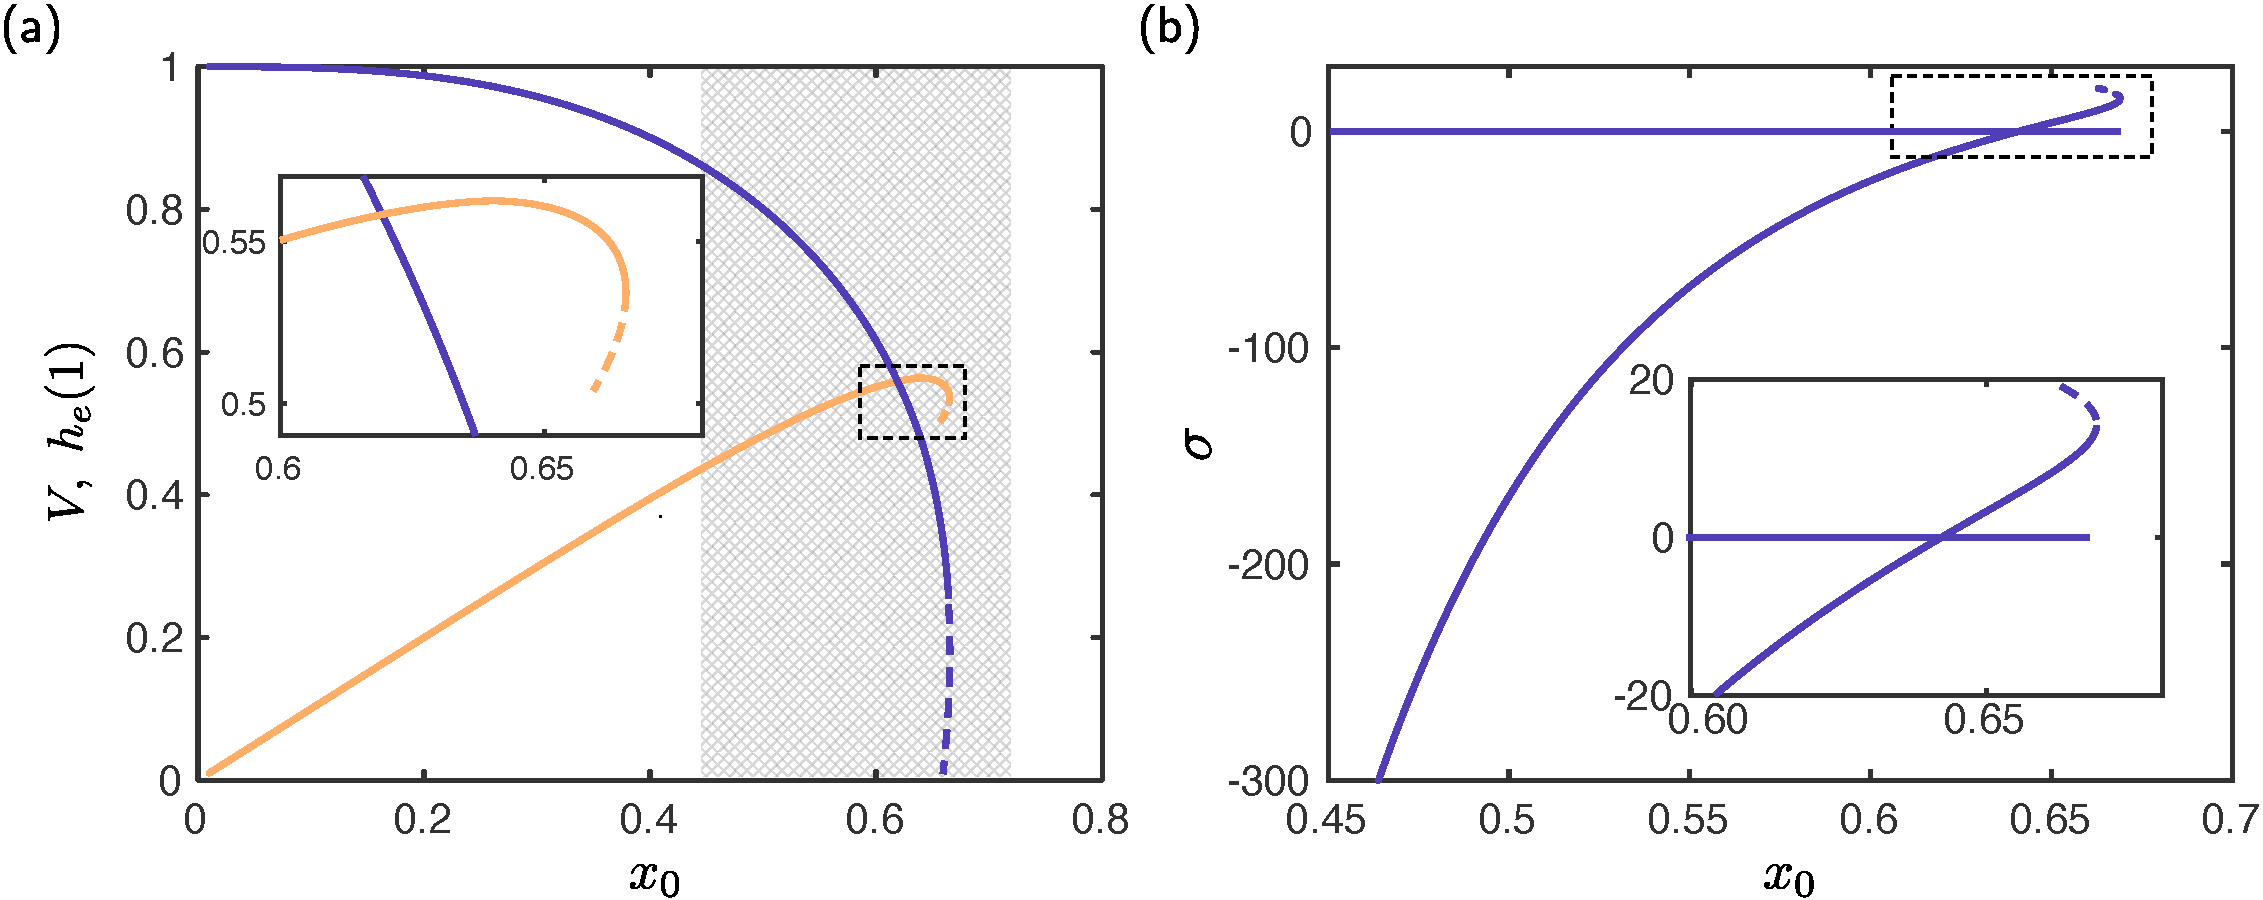
\includegraphics[width =0.98\textwidth]{tv12_stability_nu_is_10_by_x0}
\caption{(a) Equilibrium volume  $V$ (orange curve) and free end channel width $h_e(x = 1)$ (purple curve) in steady solutions of the model equations~\eqref{E:InstabilityChapter:Modelling:NonDim:PDE1}--\eqref{E:InstabilityChapter:Modelling:NonDim:Kinematic} with $\nu = 10$. The solid and dashed parts of the curve corresponds to the `$+$' and `$-$' roots of~\eqref{E:InstabilityChapter:FlatInterface:NoCond:MeniscusWidth}, respectively. Inset: a close up of the section of the main figure indicated by the black dashed box, in which multiple equilibria with the same meniscus position exist. (b) Growth rate $\sigma_u$ of uniform perturbations (i.e.~of the form~\eqref{E:InstabilityChapter:FlatInterface:NoCond:uniform_perturbation}) to the equilibria indicated by the points in (a) that lie within the hatched box. Each equilibria is associated with two values of $\sigma_u$, one of which is always zero. Inset: a close up of the section of the main figure indicated by the black dashed box.}\label{fig:InstabilityChapter:FlatInterface:NoCond:Tv12_analogue}
\end{figure}

The `$-$' root exists only for small band of sufficiently large meniscus position $x_0$ (or, equivalently, for sufficiently large $V$, see Figure~\ref{fig:InstabilityChapter:FlatInterface:NoCond:Tv12_analogue}(a)) (the `$-$' root violates the no-touching condition~\eqref{E:InstabilityChapter:FlatInterface:NoCond:NoTouchCond} for smaller $x_0$), whilst the `$+$' root exists for a large range of $x_0$ including $0$.  Further, the `$+$' root is associated with smaller deformations; in particular, if
\begin{equation}\label{E:InstabilityChapter:FlatInterface:NoCond:epsilon_def}
\epsilon \coloneqq |\nu| V^4 \ll 1,
\end{equation}
then from~\eqref{E:InstabilityChapter:FlatInterface:NoCond:MeniscusDispQuadratic}, we find that $h_m^+ = 1 + \mathcal{O}(\epsilon)$, whilst $h_m^- = \mathcal{O}(\epsilon)$. If we take the $`+'$ root in this small deformation case, then from~\eqref{E:InstabilityChapter:FlatInterface:NoCond:MeniscusDispQuadratic} we find that the meniscus position satisfies
\begin{equation}\label{E:InstabilityChapter:FlatInterface:NoCond:Asymptotic_x0_to_V}
 x_0 = V\left[1 + \frac{\mathrm{sgn}(\nu)\epsilon}{20}  + \mathcal{O}(\epsilon^2)\right],
\end{equation}
where $\mathrm{sgn}$ is the signum function. The associated channel shape is
\begin{equation}\label{E:InstabilityChapter:FlatInterface:NoCond:Asymptotic_channel_shape}
h_e(x) = 1 + \mathrm{sgn}(\nu)\epsilon\psi \left(\frac{x}{V}\right) + \mathcal{O}(\epsilon^2),\qquad \psi(s) = \frac{-1}{8} + \frac{1}{24}\left[4(1-s) - (1-s)^4\right].
\end{equation} Equation~\eqref{E:InstabilityChapter:FlatInterface:NoCond:Asymptotic_x0_to_V} demonstrates that the meniscus position and the volume are approximately equal when deformations are small, which is encoded by~\eqref{E:InstabilityChapter:FlatInterface:NoCond:epsilon_def}. Expressions~\eqref{E:InstabilityChapter:FlatInterface:NoCond:Asymptotic_x0_to_V} and~\eqref{E:InstabilityChapter:FlatInterface:NoCond:Asymptotic_channel_shape} will be important when we formally consider the case of small deformations in due course.

Before moving on to consider the stability of these equilibria to in-plane perturbations, we briefly consider their stability to \textit{uniform} perturbations (or, equivalently to in-plane perturbations with zero wavenumber). In this scenario, the instability mechanism is somewhat simpler than that described in \S\ref{S:InstabilityChapter:Mechanism:Elasticity}: the meniscus would like to advance to wet the beams over a longer length, but the additional deformation that results will incur a bending energy penalty.

Following Taroni and Vella, we probe the stability of the equilibria by substituting
\begin{equation}\label{E:InstabilityChapter:FlatInterface:NoCond:uniform_perturbation}
h = h_e(x) + \varepsilon \Lambda_0(x)\exp(\sigma_u t),~p = p_0 + \varepsilon \Pi_0(x)\exp(\sigma_u t),~ x_0 = x_0 +  \varepsilon \exp(\sigma_u t),
\end{equation}
where $\varepsilon \ll 1$ is arbitrary, into the model equations~\eqref{E:InstabilityChapter:Modelling:NonDim:ClampedBC}--\eqref{E:InstabilityChapter:Modelling:NonDim:Kinematic}; linearizing in $\varepsilon$ yields a boundary value problem which can be solved numerically to obtain the growth rate $\sigma_u$ for a given $\nu$ and $V$ (the numerical procedure is described in following section for in-plane perturbations of any wavenumber).

For each of the roots of~\eqref{E:InstabilityChapter:FlatInterface:NoCond:MeniscusWidth}, this boundary value problem has two solutions, resulting in two unique values of $\sigma_u$ for each equilibrium (Figure~\ref{fig:InstabilityChapter:FlatInterface:NoCond:Tv12_analogue}(b)). One of these growth rates, $\sigma_u^2$, is always zero; the corresponding solution does not conserve mass -- it refers to a uniform advance of the meniscus with no corresponding change in channel shape.

The second of these growth rates, $\sigma_u^1$, is negative and large in magnitude for small $x_0$ (Figure~\ref{fig:InstabilityChapter:FlatInterface:NoCond:Tv12_analogue}(b)). Increasing $x_0$ is accompanied by an increase in $\sigma_u^1$ because  the bending penalty incurred by the perturbation is reduced when the meniscus is closer to the free end, when the channel is effectively softer. For a small range of $x_0$, the equilibrium corresponding to the `$+$' root in~\eqref{E:InstabilityChapter:FlatInterface:NoCond:MeniscusWidth} are unstable (the growth of perturbations is positive), whilst those corresponding to the `$-$' root are always unstable.

As we a primarily interested in low volume configurations, we shall henceforth ignore the equilibria corresponding to the `$-$' root in~\eqref{E:InstabilityChapter:FlatInterface:NoCond:MeniscusWidth}.


\subsection{Periodic perturbations}\label{S:InstabilityChapter:SlowCondensation:PeriodicPerturbations}
\renewcommand{\Lambda}{H}
\renewcommand{\Pi}{P}
To analyze the linear stability of these equilibria to perturbations with an in-plane component, we let
\begin{align}
h &= h_e(x) + \varepsilon \Lambda(x)\exp(\sigma t + i k y),\label{E:InstabilityChapter:SlowCondensation:Periodic:Perturbation1} \\
 p &= p_m + \varepsilon \Pi(x)\exp(\sigma t + i k y),\\ x_m  &= x_0 +  \varepsilon \exp(\sigma t + i k y),\label{E:InstabilityChapter:SlowCondensation:Periodic:Perturbation3}
\end{align}
with $\varepsilon$ again arbitrary. Substituting~\eqref{E:InstabilityChapter:SlowCondensation:Periodic:Perturbation1}--\eqref{E:InstabilityChapter:SlowCondensation:Periodic:Perturbation3} into the model equations~\eqref{E:InstabilityChapter:Modelling:NonDim:ClampedBC}--\eqref{E:InstabilityChapter:Modelling:NonDim:Kinematic} (with $C = 0$) and linearizing yields a coupled boundary value problem (BVP) for $\Lambda$ and $\Pi$:

\begin{align}
\sigma \Lambda &=  \frac{h_e^2}{3|\nu|}\left[3\dd{h_e}{x} \dd{\Pi}{x} + h_e\left(\dd{^2 \Pi}{x^2} - k^2 \Pi\right)\right] & &0 < x < x_0,\label{E:InstabilityChapter:SlowCondensation:Periodic:ODEwet}\\
0 &= \Pi & &x_0 < x < 1,\label{E:InstabilityChapter:SlowCondensation:Periodic:ODEdry}\\
\Pi &= \dd{^4 \Lambda}{x^4} - 2k^2 \dd{^2 \Lambda}{x^2} + k^4 \Lambda & & 0 < x <1.\label{E:InstabilityChapter:SlowCondensation:Periodic:pressure2shape}
\end{align}
The boundary conditions on~\eqref{E:InstabilityChapter:SlowCondensation:Periodic:ODEwet}--\eqref{E:InstabilityChapter:SlowCondensation:Periodic:pressure2shape} are
\begin{align}
\Lambda &= 0 = \dd{\Lambda}{x} = \dd{\Pi}{x} & &\text{at}~x = 0,\label{E:InstabilityChapter:SlowCondensation:Periodic:BC_at_0}\\
\Pi &= \frac{\nu}{h_m^2}\left(\dd{h_e}{x} + \Lambda\right) + \nu \aspect k^2 & &\text{at}~x = x_0,\label{E:InstabilityChapter:SlowCondensation:Periodic:pressure_bc}\\
\dd{^2 \Lambda}{x^2} - \poisson k^2
\Lambda &= 0 = \dd{^3 \Lambda}{x^3} - (2-\poisson)k^2 \dd{\Lambda}{x} & &\text{at}~x = 1,\label{E:InstabilityChapter:SlowCondensation:Periodic:BC_at_1}
\end{align}
\begin{equation}\label{E:InstabilityChapter:SlowCondensation:Periodic:jump_conds}
\left[\Lambda\right]\jump{x_0}= \left[\dd{\Lambda}{x}\right]\jump{x_0} = \left[\dd{^2\Lambda}{x^2}\right]\jump{x_0}= 0, \quad\left[\dd{^3 \Lambda}{x^3}\right]\jump{x_0} = \frac{\nu}{h_m },
\end{equation}
The growth rate $\sigma$ satisfies
\begin{equation}\label{E:InstabilityChapter:SlowCondensation:Periodic:kinematic}
\sigma = -\frac{h_m^2}{3|\nu|}\left.\ddp{\Pi}{x}\right|_{x = x_0}.
\end{equation}

The terms on the right hand side of~\eqref{E:InstabilityChapter:SlowCondensation:Periodic:pressure_bc} elucidate the mechanism described in \S\ref{S:InstabilityChapter:Mechanism:Elasticity}; in order, they correspond to the transverse curvature changes arising from channel tapering set by the base state, transverse changes arising from the elastic response to the perturbation, and the stabilizing in-plane curvature of the perturbation. 

\subsubsection{Numerical results}\label{S:InstabilityChapter:NoCond:Numerics}
To solve the BVP numerically, we first write it as a first order system of ODEs; we solve this system using the BVP4C routine implemented in \textsc{matlab}~\citep{Kierzenka2001BVP}.
As for the uniform perturbation discussed in the previous section, the problem has two solutions and which is of these is returned depends on the proximity to the initial guess for $\sigma$. The corresponding growth rates $\sigma_i, i = 1,2$ originate from $\sigma_u^i$ (i.e.~$\sigma_i(k= 0) = \sigma_u^i$). In particular, those solutions on the $\sigma_2$ branch originate from the solution that does not conserve mass, so would need mass adding; with $k \neq 0$, however, it is possible to move mass in the $y$-direction.

It is the $\sigma_2$ that is of most interest here: this branch shows positive growth rates (Figure~\ref{fig:InstabilityChapter:SlowCondensation:GrowthRates}(a)); the branch originating at $\sigma_u^1$ has very high decay rates even for small $k$. To reflect this, we drop the index and take $\sigma =  \sigma_2$ henceforth.

%Generic features: growth rate positive for sufficiently small $\khat$, and $h_1(x_0) < 0$
Dispersion relations $\sigma(k)$ are obtained by solving the BVP~\eqref{E:InstabilityChapter:SlowCondensation:Periodic:ODEwet}--\eqref{E:InstabilityChapter:SlowCondensation:Periodic:kinematic} numerically over a range of different $k$ values, and are shown in Figure~\ref{fig:InstabilityChapter:SlowCondensation:GrowthRates} for different cross sectional volumes $V = V(x_0)$. We see that $\sigma > 0$ for sufficiently small wavenumbers -- an observation that is generic in numerical solutions of the BVP. In addition, $\sigma\sim k^2$ as $k \to 0$ (Figure~\ref{fig:InstabilityChapter:SlowCondensation:GrowthRates}(b)) as suggested by the scaling argument~\eqref{E:InstabilityChapter:Scaling:amplitude_ode}. (We shall derive this formally in the case of small deformations shortly.)

\begin{figure}[t]
\centering
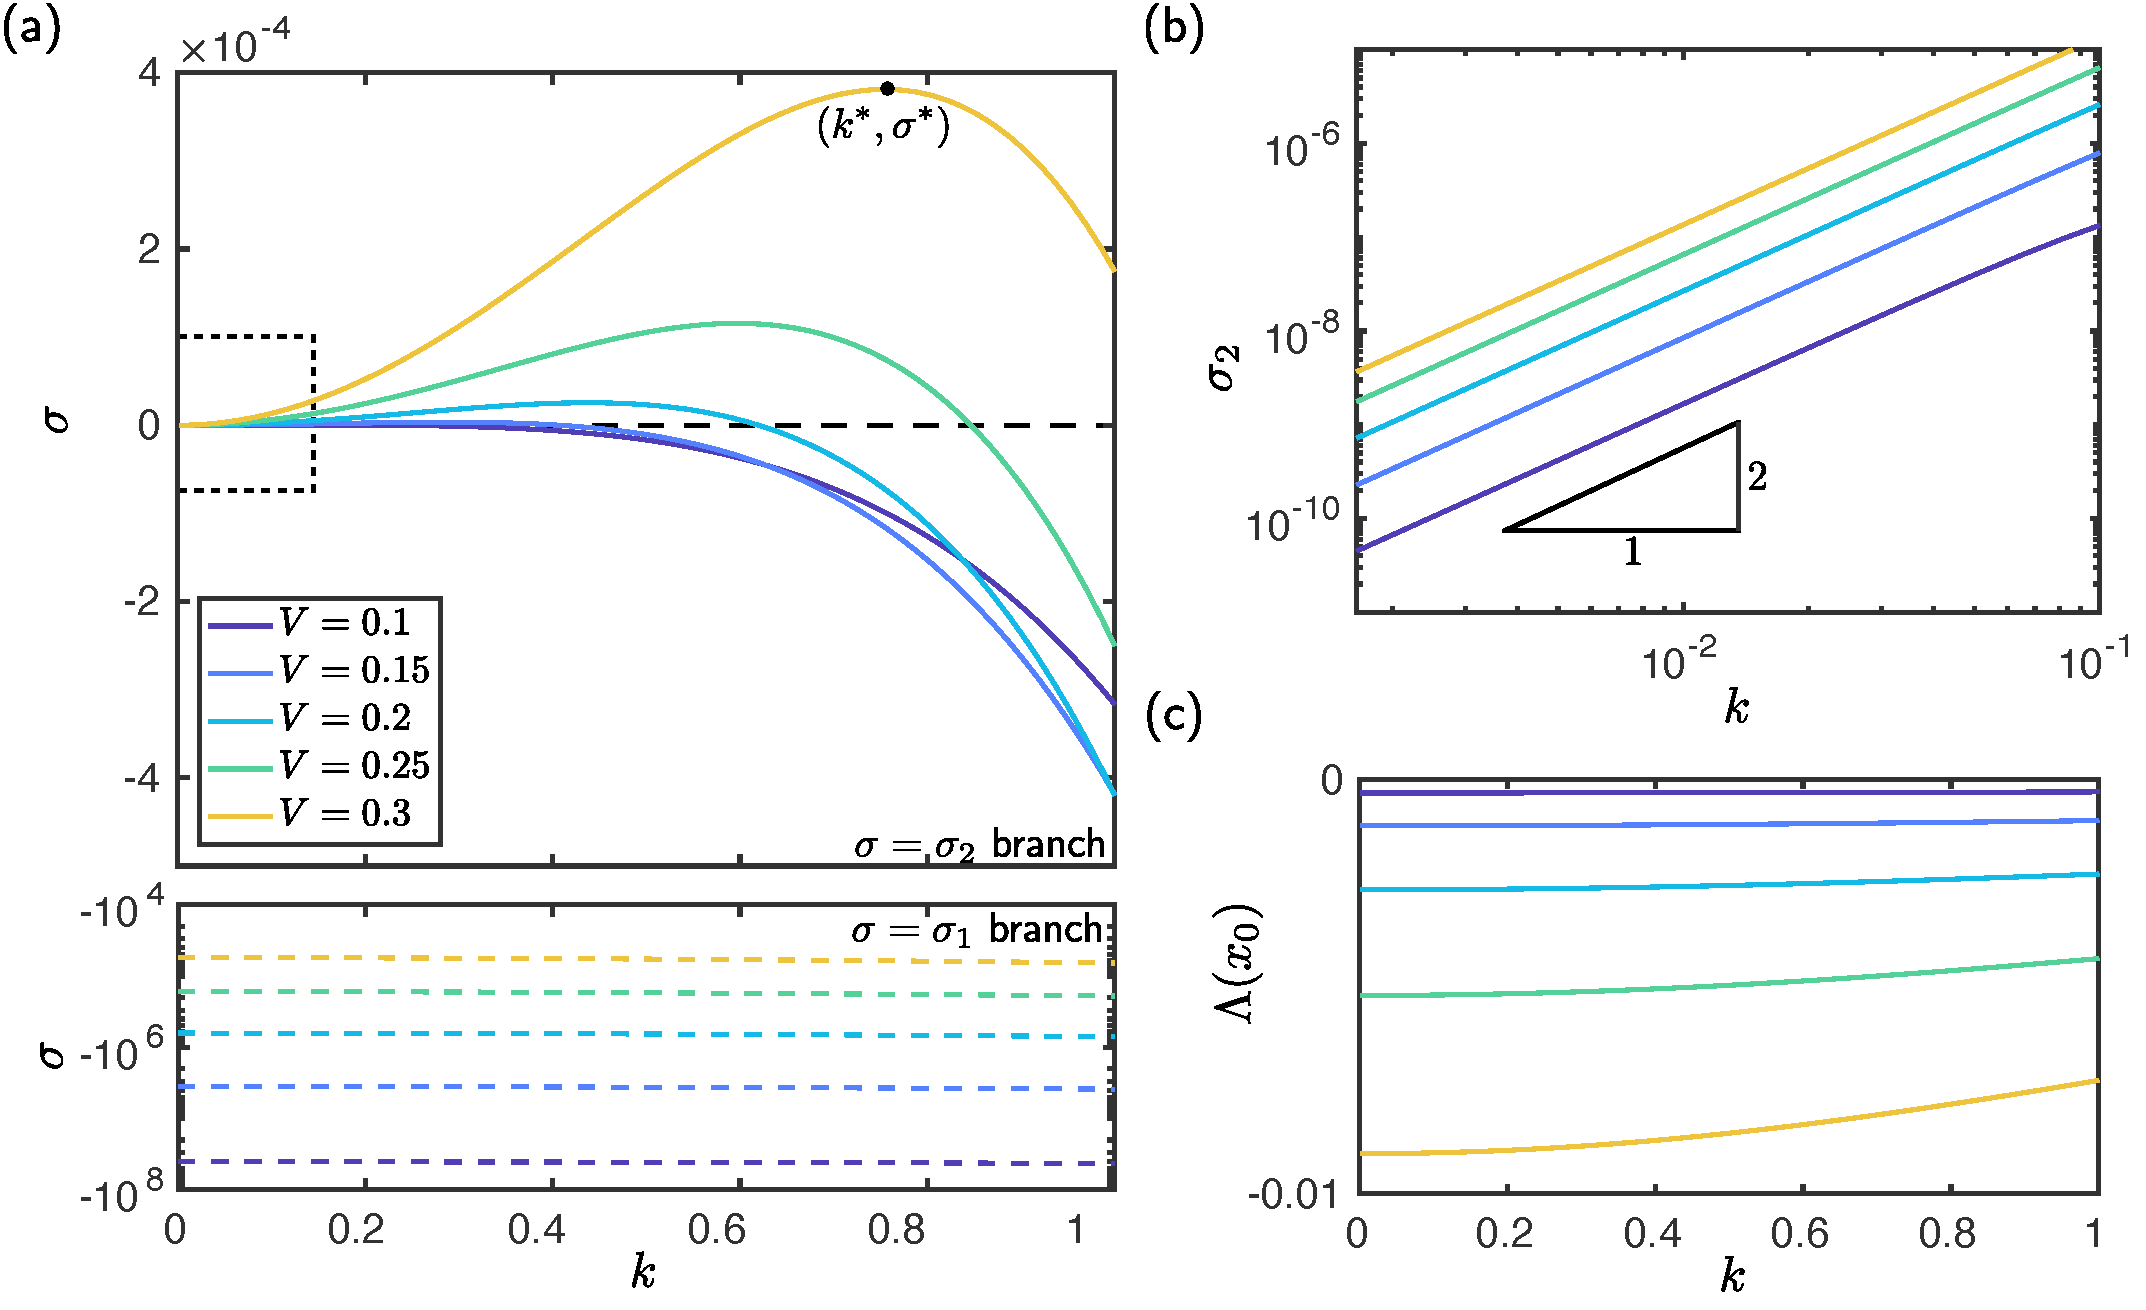
\includegraphics[width = 0.98\textwidth]{Growth_rates}
\caption{Numerical solutions of the boundary value problem arising from periodic perturbations with wavenumber $k$ to an equilibrium with cross-sectional volume $V$ (values indicated by the legend), $\nu = 1$ and $\aspect = 0.01$. (a) Growth rates $\sigma_{i}, i = 1,2$ of the perturbation shown as solid ($i = 1$) and dashed ($i = 2$) lines. The black dashed line indicates $\sigma = 0$. Note that the bottom axis uses a semi-logarithmic scale to allow all the data to be seen. (b) Zoom in on the small $k$ region of the $\sigma_1$ curve in the dashed box in (a), plotted on logarithmic axes. (c) Value of shape perturbation at the interface. Colours are as in (a) and (b).}
\label{fig:InstabilityChapter:SlowCondensation:GrowthRates}
\end{figure}


Another generic feature of numerical solutions of the BVP is that the perturbation to the shape is negative at the meniscus, $\Lambda(x_0) <0$  (Figure~\ref{fig:InstabilityChapter:SlowCondensation:GrowthRates}(c)): the channel deformation of the base state is enhanced at protrusions and reduced at invaginations. (For non-wetting configurations with $\nu <0$, $\Lambda(x_0)$ is positive, again corresponding to enhanced deformation at protrusions.)

For the parameter values used in Figure~\ref{fig:InstabilityChapter:SlowCondensation:GrowthRates}, the fastest growing mode, denoted $k^*$, and the corresponding growth rate $\sigma^* = \sigma(k^*)$, both increase with cross-sectional volume $V$. This is in qualitative agreement with the scaling argument~\eqref{E:InstabilityChapter:Scaling:SigmaScaling1}, which, after non-dimensionalizing with the length scale $L$ and time scale $\tau_c$, suggests the typical scales
\begin{equation}\label{E:InstabilityChapter:SlowCondensation:NumericalSols:DimensionlessScalings}
k_c  = \left(\frac{\nu V^3}{a}\right)^{1/2}, \qquad \sigma_c = \frac{\nu^2 V^7}{|a|}.
\end{equation}

For a quantitative assessment of the scaling argument, we rescale the numerically obtained dispersion relations $\sigma(k)$ according to~\eqref{E:InstabilityChapter:SlowCondensation:NumericalSols:DimensionlessScalings} (Figure~\ref{fig:InstabilityChapter:SlowCondensation:CollapsedGrowthRates}(a)). Here we see that the data collapse onto a universal curve for $\nu \ll 1$ (indicated by dark shades in Figure~\ref{fig:InstabilityChapter:SlowCondensation:CollapsedGrowthRates}(a)), but deviate when $\nu \gg 1$ (light shades). In addition, the deviation occurs sooner (i.e. at lower $\nu$ values) for larger volume $V$ where the base state deformation is expected to be larger. To predict the envelope enclosing the curves $\sigma/\sigma_c$ we now perform an asymptotic expansion of the BVP~\eqref{E:InstabilityChapter:SlowCondensation:Periodic:ODEwet}--\eqref{E:InstabilityChapter:SlowCondensation:Periodic:kinematic} in the limit of small deformations.

\begin{figure}[t]
\centering
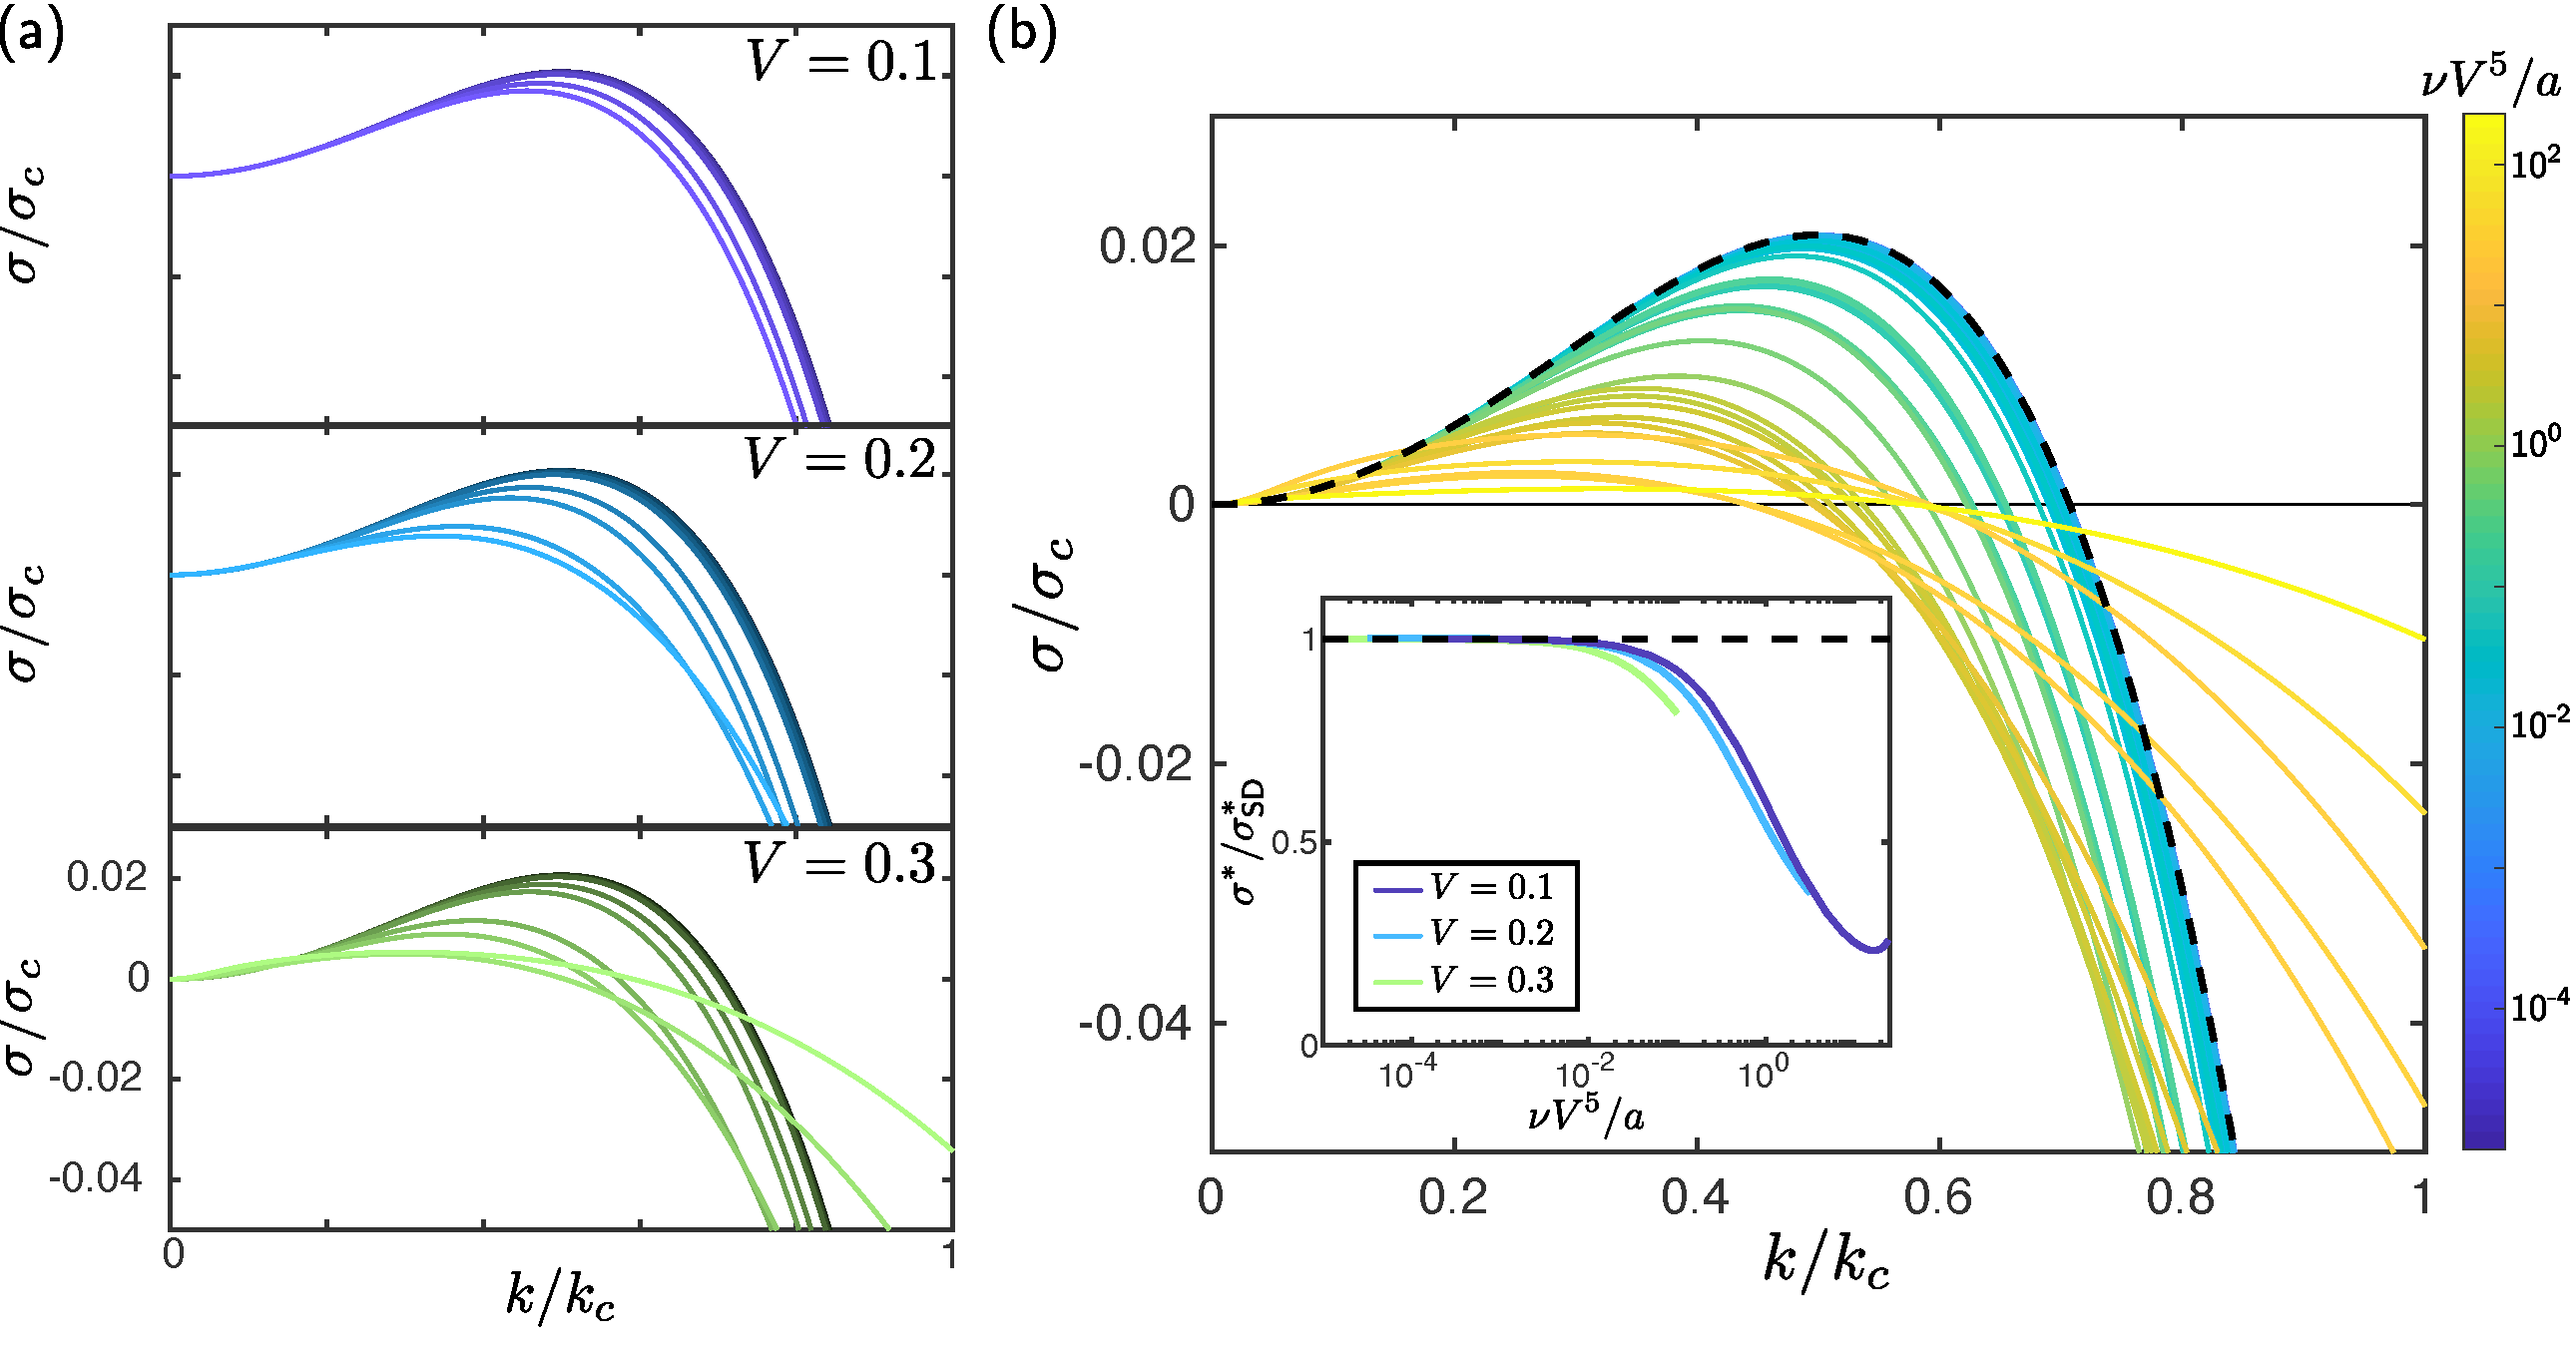
\includegraphics[width = \textwidth]{Collapsed_growth_rates}
\caption{(a) Numerically obtained dispersion relations $\sigma(k)$ rescaled according to~\eqref{E:InstabilityChapter:SlowCondensation:NumericalSols:DimensionlessScalings}. The value of the cross sectional volume $V$ used is indicated in each plot, and here $\aspect = 0.01$. Each curve corresponds to a different value of $\nu$, taking logarithmically spaced values between $10^{-2}$ and $10^{2}$; darker shaded curves corresponds to lower values of $\nu$. (b) Rescaled growth rates shown from (a) plotted on top of one another, and coloured according to $\nu V^5 /a$ (indicated by the colour bar); the results for $\nu V^5 /a \lesssim 10^{-2}$ are indistinguishable from the black dashed curve, which represents the asymptotic result~\eqref{E:InstabilityChapter:SlowCondensation:Asymptotics:SigmaResult}. Inset: semilogarithmic plot of the ratio between numerically obtained values of the maximum growth rate $\sigma^*$ and the asymptotic prediction $\sigma^*_{\textsf{SD}}$ given by~\eqref{E:InstabilityChapter:SlowCondensation:Asymptotics:FastestGrowingMode}.}
\label{fig:InstabilityChapter:SlowCondensation:CollapsedGrowthRates}
\end{figure}


\subsection{Asymptotics for small deformations}\label{S:InstabilityChapter:NoCondensation:SmallDeformations}
In this section, we provide details of an asymptotic analysis of the boundary value problem~\eqref{E:InstabilityChapter:SlowCondensation:Periodic:ODEwet}--\eqref{E:InstabilityChapter:SlowCondensation:Periodic:kinematic} in the case of small deformations. We aim to predict the envelope of growth rate curves in Figure~\ref{fig:InstabilityChapter:SlowCondensation:CollapsedGrowthRates} and thus predict the fastest growing mode and corresponding growth rate in this limit. Here we give an outline of the asymptotic analysis -- further details can be found in Appendix~\ref{A:InstabilityChapter:SmallDeformationAsymptotics}.

\subsubsection{Qualitative description of analysis}
As alluded to in \S\ref{S:InstabilityChapter:BaseState:Equilibria}, we encode small deformations by considering
\begin{equation}
\epsilon  = |\nu| V^4 \ll 1.
\end{equation}

The first step in the asymptotic analysis is to rescale the wavenumber by introducing $\K =k/k_c \sim \mathcal{O}(1)$ (when $k \sim k_c$ the two curvature contributions in the pressure boundary condition~\eqref{E:InstabilityChapter:SlowCondensation:Periodic:pressure_bc} balance). We anticipate the majority of the bending deformation occurs in the wet region $0 < x < x_0 = V + \mathcal{O}(\epsilon)$, and introduce the rescaled spatial variable $X = x/V$ to reflect this. In doing so,  the parameter $\param = \nu V^5 / a  = \epsilon  V/|a|$ naturally appears; $\xi$ describes the relative sizes of increases in-plane and transverse bending energies when the equilibrium is subject to a perturbation with wavenumber $k \sim k_c$. To see this we note that the typical (dimensionless) in-plane and transverse wall curvatures induced by this perturbation are
\begin{equation}
\kappa_{\text{in-plane}} \sim k_c^2 \Delta h \sim \frac{\nu V^3}{a} \Delta h \quad \text{and}\quad \kappa_{\text{transverse}} \sim \frac{\Delta h}{x_0^2} \sim  \frac{\Delta h}{V^2},
\end{equation}
where $\Delta h$ is the typical change in channel thickness that results from the perturbation. The corresponding dimensionless bending energies are
\begin{align}
E_{\text{in-plane}} &\sim \frac{\left(\kappa_{\text{in-plane}}\right)^2}{k_c} \sim \left( \frac{\nu V^3}{a}\right)^{3/2}(\Delta h)^2,\\ 
E_{\text{transverse}} &\sim x_0 \left(\kappa_{\text{transverse}}\right)^2 \sim \frac{(\Delta h)^2}{V^3},
\end{align}
whose ratio is
\begin{equation}
\frac{E_{\text{in-plane}}}{ E_{\text{transverse}}}
\sim \param^{3/2}.
\end{equation}

To make progress, we consider the limit $\param \to 0$. We pose a bivariate asymptotic expansion of the perturbation to the channel shape, $\Lambda$, the perturbation to the pressure, $\Pi$, and the growth rate, $\sigma$, in both $\epsilon$ and $\param$, using subscript $\left\{i,j\right\}$ to denote the term at $\mathcal{O}(\param^i \epsilon^j)$:
\begin{align}
\Lambda(X) &=    \Lambda_{0,0} + \param \Lambda_{1,0} + \epsilon \Lambda_{0,1} +  \param^2 \Lambda_{2,0} + \param \epsilon \Lambda_{1,1} + \epsilon^2 \Lambda_{0,2} + \dots,\label{E:InstabilityChapter:SlowCondensation:Asymptotics:ExpansionH} \\
\Pi(X) &=  \Pi_{0,0} + \param \Pi_{1,0} + \epsilon \Pi_{0,1} +  \param^2\Pi_{2,0} + \param \epsilon \Pi_{1,1} + \epsilon^2 \Pi_{0,2}+\dots,\label{E:InstabilityChapter:SlowCondensation:Asymptotics:ExpansionP} \\
\sigma(k) &= \sigma_{0,0} + \param \sigma_{1,0} + \epsilon \sigma_{0,1} +  \param^2 \sigma_{2,0} + \param \epsilon \sigma_{1,1} + \epsilon^2 \sigma_{0,2} + \dots. \label{E:InstabilityChapter:SlowCondensation:Asymptotics:ExpansionSigma}
\end{align}

\subsubsection{Results}
The particular hierarchy of problems arising from the asymptotic expansion~\eqref{E:InstabilityChapter:SlowCondensation:Asymptotics:ExpansionH}--\eqref{E:InstabilityChapter:SlowCondensation:Asymptotics:ExpansionSigma} depends on the relative sizes of $\epsilon$ and $\param$, but we must ensure that $V \gg |\aspect|$ for lubrication theory to remain valid, and therefore
$\param  = \epsilon (V/|a|) \gg \epsilon$ (in Appendix~\ref{A:InstabilityChapter:SmallDeformationAsymptotics}, we present the hierarchy of problems for the case $\epsilon \sim \param^2$). The leading order ($\mathcal{O}(1)$) and first order ($\mathcal{O}(\param)$) problems are, however, independent of the relationship between $\epsilon$ and $\param$.


In the leading order and first order problems, the pressure profile is a linear function of $X$. However, to satisfy the no flux condition at $X =0$, this pressure perturbation is, in fact, constant and thus offers no contribution to $\sigma$, i.e.
\begin{equation}
\sigma_{0,0} = 0 = \sigma_{1,0}.
\end{equation}
We find the leading order contribution to the perturbation to the channel shape to be
\begin{equation}
\Lambda_{0,0} =\nu V^3 \times \begin{cases}
\frac{X^2}{6}(X - 3) & 0 < X < 1,\\
\frac{1}{6}(1-X) & 1 < X < 1/V.
\end{cases}
\end{equation}
The leading order solution reflects a shear arising from the base state pressure (magnitude $\nu$) acting over a length equal to the amplitude of the perturbation, to deform the wall over a length comparable to $V$ (the shear force is the third derivative of the beam shape). Note that $\Lambda_{0,0}(X=1) < 0$ -- this allows us to verify that $\Lambda(x = x_0) < 0$ in the limit of small deformations, $|\nu| V^4 \to 0$ (as suggested in the previous section). We find the Poisson's ratio $\poisson$ in the first order term, $\Lambda_{1,0}$, but not in the leading order term, $\Lambda_{0,0}$, demonstrating that the contribution from the dry region enters at lower order (the Poisson's ratio only enters the problem via the boundary conditions on the dry region, at $x = 1$).

Despite the dependence of the hierarchy of problems on the relationship between $\epsilon$ and $\param$, the first non-zero term in the expansion of $\sigma$~\eqref{E:InstabilityChapter:SlowCondensation:Asymptotics:ExpansionSigma} is
\begin{equation}\label{E:InstabilityChapter:SlowCondensation:Asymptotics:LeadingOrderSigma}
\sigma_{1,1} = \frac{K^2\left(1-2K^2\right)}{6V^2},
\end{equation}
regardless of the relationship between $\epsilon$ and $\param$. (The first non-zero term in the expansion~\eqref{E:InstabilityChapter:SlowCondensation:Asymptotics:ExpansionP} is the $\mathcal{O}(\epsilon)$ term, $\Pi_{0,1}$, because the terms corresponding to the destabilizing transverse curvature, and stabilizing in-plane curvature contributions to the pressure enter at this order.  However, we find that $\Pi_{0,1}$ is constant, and the first term in~\eqref{E:InstabilityChapter:SlowCondensation:Asymptotics:ExpansionP} with a non-zero gradient -- which sets the growth rate -- comes in at the next order, $\mathcal{O}(\epsilon \param)$.)

Noting that $\sigma_c = \epsilon\param/V^2$ and substituting~\eqref{E:InstabilityChapter:SlowCondensation:Asymptotics:LeadingOrderSigma} in to the expansion~\eqref{E:InstabilityChapter:SlowCondensation:Asymptotics:ExpansionSigma}, gives
\begin{equation}\label{E:InstabilityChapter:SlowCondensation:Asymptotics:SigmaResult}
\frac{\sigma(K)}{\sigma_c} =  \frac{K^2\left(1-2K^2 \right)}{6}  + \mathcal{O}(\param).
\end{equation}
Equation~\eqref{E:InstabilityChapter:SlowCondensation:Asymptotics:SigmaResult} gives the envelope of the curves $\sigma(k)$ (Figure~\ref{fig:InstabilityChapter:SlowCondensation:CollapsedGrowthRates}(b)). Moreover, and as expected, numerical solutions with larger values of $\param = \nu V^5 /|a|$ deviate more significantly from this envelope.

By maximizing~\eqref{E:InstabilityChapter:SlowCondensation:Asymptotics:SigmaResult} with respect to $K$, we find that the small deformation estimates of the fastest growing mode, denoted $k^*_{\textsf{SD}}$, and the corresponding growth rate, denoted $\sigma^*_{\textsf{SD}}$ are
\begin{equation}\label{E:InstabilityChapter:SlowCondensation:Asymptotics:FastestGrowingMode}
\sigma^*_{\textsf{SD}}= \frac{1}{48}\sigma_c = \frac{1}{48}\frac{\nu^2 V^7}{\aspect}, \qquad k^*_{\textsf{SD}}= \frac{1}{2}k_c = \frac{1}{2}\sqrt{\frac{\nu V^3}{\aspect}}.
\end{equation}
which agree well with numerical solutions of the BVP (see inset of Figure~\ref{fig:InstabilityChapter:SlowCondensation:CollapsedGrowthRates}(b), in which perfect agreement would correspond to $y = 1$). Numerical solutions with larger values of $V$ -- and thus larger values of $\epsilon = |\nu| V^4$ for a given $\nu$ -- peel off from the asymptotic prediction~\eqref{E:InstabilityChapter:SlowCondensation:Asymptotics:FastestGrowingMode} at a lower value of $\delta$, as we would expect.

The numerically obtained values of $\sigma^*/\sigma^*_{\textsf{SD}}$ are not monotonic in $\param = \nu V^5/a$ (see the $V = 0.1$ curve in the inset of Figure~\ref{fig:InstabilityChapter:SlowCondensation:CollapsedGrowthRates}(b)). As $\param$ increases, the penalizing effect of in-plane bending tends to suppress the growth rate relative to the asymptotic result ($\sigma^*/\sigma^*_{\textsf{SD}}$ initially decreases). For a given value of $\aspect$, increases in $\param = \nu V^5/|a|$ are, however, accompanied by increases in the deformation parameter $\epsilon = |\nu| V^4$ allowing the non-linear effects of significant base state deformation to enter. Specifically, the competition between the non-linearities in channel permeability and meniscus pressure (which tend to reduce and enhance the growth rate of instability, respectively) is won by the former, and the net effect of the channel width non-linearity is to enhance the growth rate relative to $\sigma^*_{\text{SD}}$. (This is reminiscent of the `over-shooting' of the asymptotic result by numerical solutions observed in Chapter 2.)

Note that our prediction of the fastest growing mode and the corresponding growth rate are highly sensitive to the amount of liquid in the channel via the volume $V$ ($\sigma \sim V^7$ for small deformations~\eqref{E:InstabilityChapter:SlowCondensation:Asymptotics:FastestGrowingMode}); we might expect, therefore, that if the volume is changing, then the fastest growing mode will be changing as well. We turn now to consider the case of non-zero condensation to describe formally how the mode selection problem changes when the liquid is being added via condensation.

\section{The influence of condensation}
In this section, we consider the case when $C>0$, and liquid is added to the channel via condensation. We focus on how mode selection in the competing curvature instability described in the previous section, is modified by the presence of a dynamic base state and a non-constant liquid volume that result from a non-zero condensation rate.

\subsection{Base State}
With $C>0$, equilibria of the model equations~\eqref{E:InstabilityChapter:Modelling:NonDim:ClampedBC}--\eqref{E:InstabilityChapter:Modelling:NonDim:Kinematic} do not exist. In this case, the base state configurations are those with a cylindrical interface:
\begin{equation}\label{E:InstabilityChapter:BaseState:FlatInterface:FlatAnsatz}
h = h_0(x,t), \qquad p = p_0(x,t), \qquad \x_m  = \x_0(\that).
\end{equation}

Substituting~\eqref{E:InstabilityChapter:BaseState:FlatInterface:FlatAnsatz} into the model equations~\eqref{E:InstabilityChapter:Modelling:NonDim:ClampedBC}--\eqref{E:InstabilityChapter:Modelling:NonDim:Kinematic}  results in a system of spatially one dimensional PDEs:
\begin{align}
\ddp{h_0}{t} & = \frac{1}{3|\nu|}\ddp{}{x}\left(h_0^3 \ddp{p_0}{x}\right) & &0 < x < x_0,\label{E:InstabilityChapter:BaseState:FlatInterface:PDEwet}\\
 p_0 &=0 & & x_0 < x < 1,\label{E:InstabilityChapter:BaseState:FlatInterface:PDEdry}\\
p_0 &= \ddp{^4 h_0}{x^4} & & 0 < x < 1.\label{E:InstabilityChapter:BaseState:FlatInterface:pressure2shape}
\end{align}
with boundary conditions
\begin{align}
h_0 &= 1, ~\ddp{h_0}{x} = 0, ~\ddp{p_0}{x} = 0 & &\text{at}~x = 0,\label{E:InstabilityChapter:BaseState:FlatInterface:bc0}\\
p_0 &= -\frac{\nu}{h_0}& &\text{at}~x = x_0,\label{E:InstabilityChapter:BaseState:FlatInterface:pressurebc}\\
\ddp{^2 h_0}{x^2} &=0,~ \ddp{^3 h_0}{x^3} = 0 & &\text{at}~x = 1,\label{E:InstabilityChapter:BaseState:FlatInterface:bc1}
\end{align}
\begin{equation}\label{E:InstabilityChapter:BaseState:FlatInterface:jumpbc}
\left[h_0\right]_{x_0^-}^{x_0^+} = \left[\ddp{h_0}{x}\right]_{x_0^-}^{x_0^+}   = \left[\ddp{^2 h_0}{x^2}\right]_{x_0^-}^{x_0^+} = \left[\ddp{^3 h_0}{x^3 }\right]_{x_0^-}^{x_0^+}   = 0,
\end{equation}
and a kinematic condition
\begin{equation}\label{E:InstabilityChapter:BaseState:FlatInterface:kinematicbc}
\ddp{x_0}{t} = -\frac{h_0^2}{3|\nu|}\left.\ddp{p_0}{x}\right|_{x = x_0} + C.
\end{equation}

The associated cross-sectional volume is now time-dependent,
\begin{equation}\label{E:InstabilityChapter:BaseState:FlatInterface:cross_sect_volume}
V(t) = \int_0^{x_0(t)} \h_0(x, t) ~\mathrm{d}x,
\end{equation}
and its initial value is denoted by $V_0 = V(t = 0)$.
We take the pressure and channel shape from the $C = 0$ equilibrium that has volume $V = V_0$ (as described in \S\ref{S:InstabilityChapter:BaseState:Equilibria}) to be the initial condition on~\eqref{E:InstabilityChapter:BaseState:FlatInterface:PDEwet}--\eqref{E:InstabilityChapter:BaseState:FlatInterface:kinematicbc} (this implicitly specifies the initial condition $x_0(t=0)$).

\subsubsection{Base state dynamics}\label{S:InstabilityChapter:WithCondensation:BaseStateDynamics}
Before moving on to analyze the stability of these base states to in-plane perturbations, we consider how the condensation rate affects their dynamic behaviour by solving equations~\eqref{E:InstabilityChapter:BaseState:FlatInterface:PDEwet}--\eqref{E:InstabilityChapter:BaseState:FlatInterface:kinematicbc} numerically. The numerical scheme used to solve these equations is very similar to that described in \S2.2 for the equations describing bendotaxis in a single flexible channel, but with a single meniscus and a no-flux boundary condition applied at $x = 0$.  Full details of this numerical scheme can be found in Appendix~\ref{A:Chapter6:Numerics}.

\begin{figure}[t]
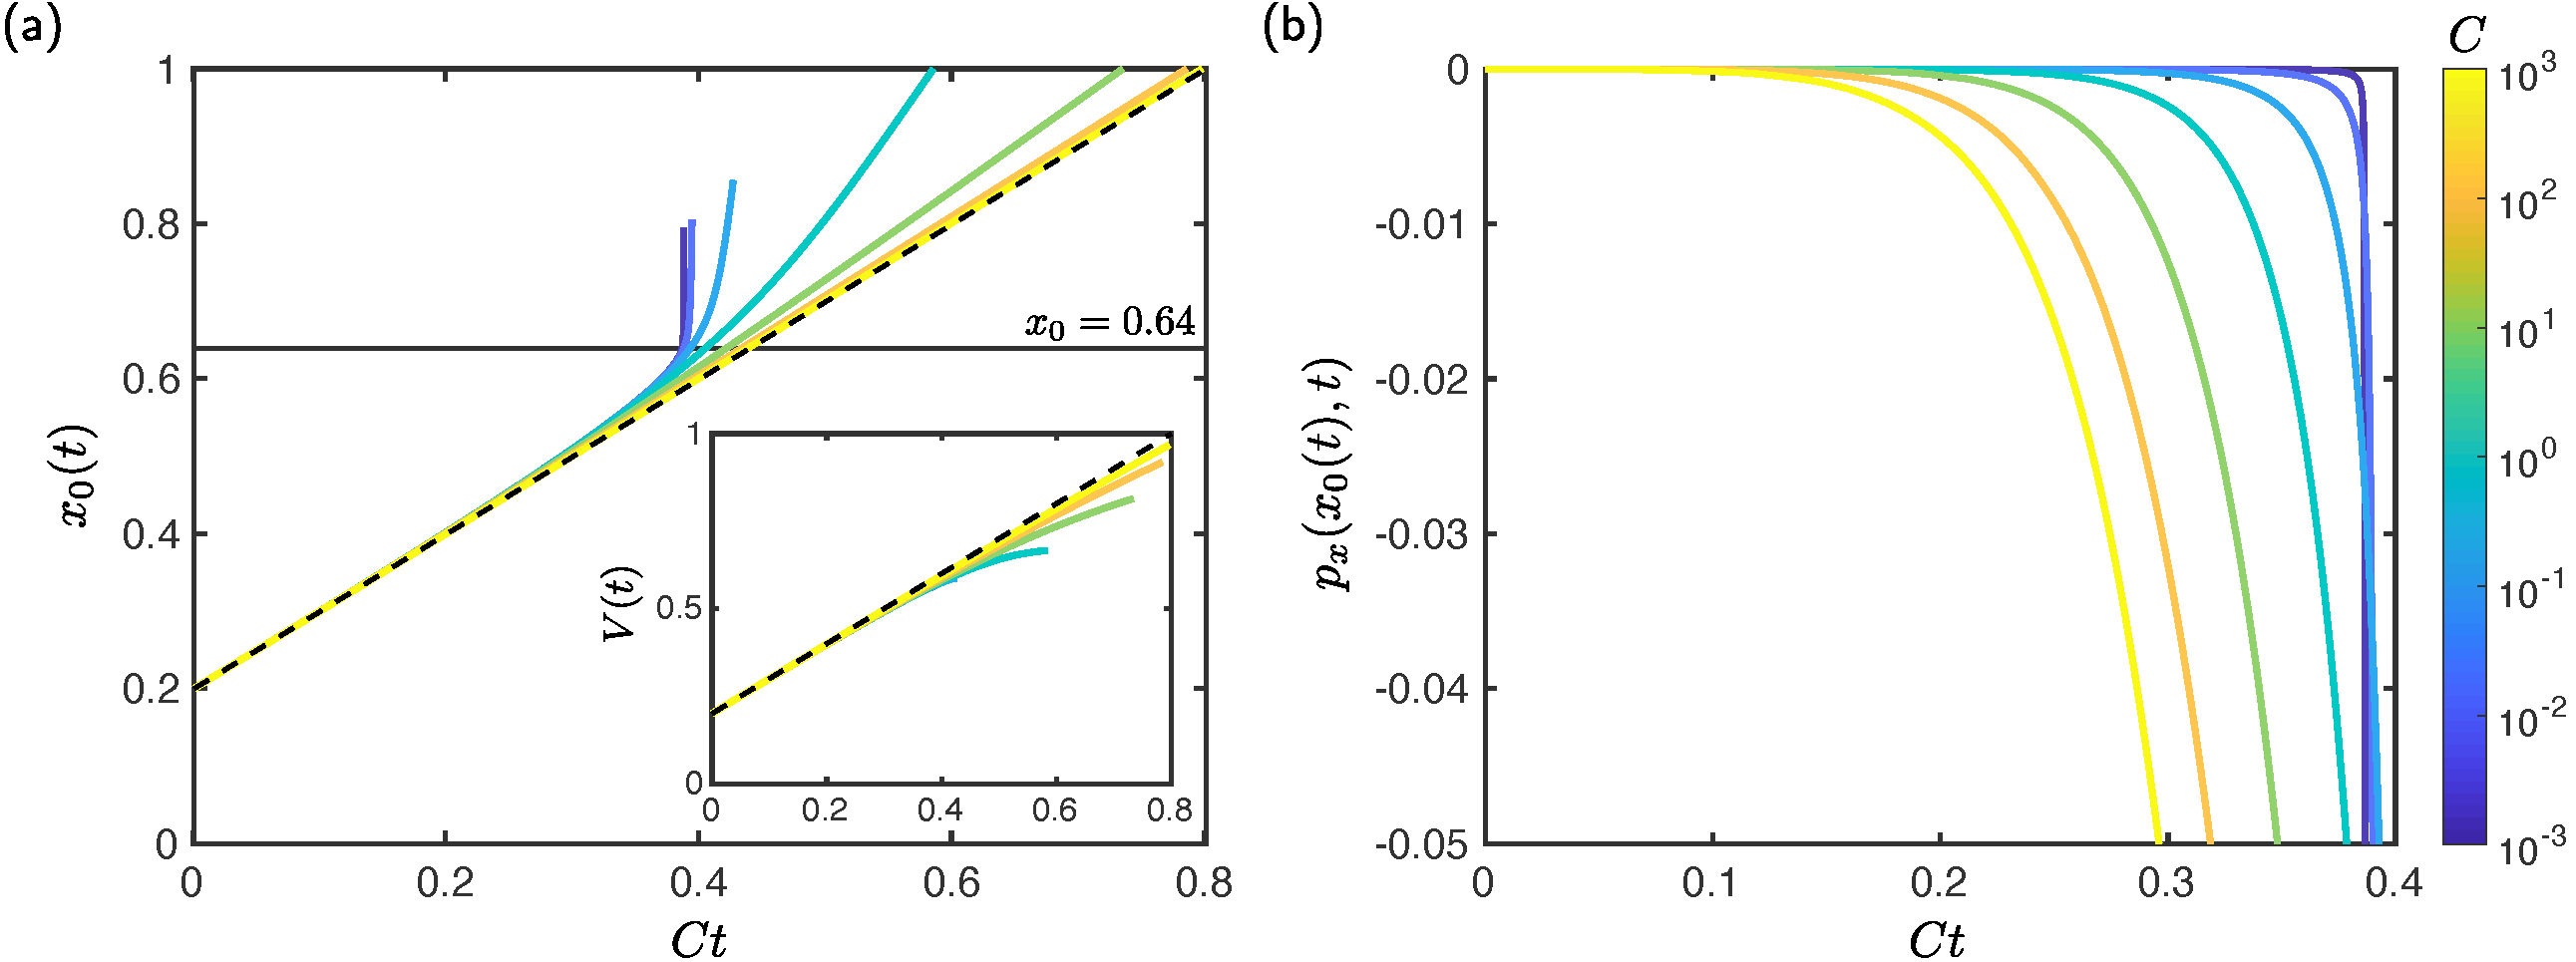
\includegraphics[width = \textwidth]{base_state_dynamicsv2}
\caption{ (a) Meniscus position, $x_0(t)$, and (b) pressure gradient at the meniscus, $p_x(x_0(t),t)$ (using subscript to denote a partial derivative with respect to $x$), in numerical solutions of base state equations~\eqref{E:InstabilityChapter:BaseState:FlatInterface:PDEwet}--\eqref{E:InstabilityChapter:BaseState:FlatInterface:kinematicbc} with $\nu = 10$, $V_0 = 0.2$. The colour of the curves indicates the condensation rate $C$ as specified in the colour bar in (b). The dashed lines in (a) indicates a linear increase in meniscus position, $x_0 = x_0(t = 0) + Ct$; the trajectories in (a) diverge from this linear prediction when $x_0 \approx 0.64$, the moment at which the corresponding $C = 0$ equilibrium goes unstable (see Figure~\ref{fig:InstabilityChapter:FlatInterface:NoCond:Tv12_analogue}). Inset: the cross sectional volume $V(t)$ in the numerical solutions of (a). The dashed line indicates $V = V_0 + Ct$. }\label{E:InstabilityChapter:WithCondensation:BaseState:Dynamics}
\end{figure}

Meniscus trajectories, $x_0(t)$, alongside the pressure gradient at the meniscus, $p_x(x_0)$, are shown in Figure~\ref{E:InstabilityChapter:WithCondensation:BaseState:Dynamics} for different values of the condensation rate $C$. The pressure gradient at the meniscus acts as a proxy for the dynamic behaviour in the base state -- deviations away from zero indicate non quasi-static behaviour of the base state.


When condensation in slow, $C \ll 1$, the behaviour can be  split into two distinct time periods. At early times  (see $t \lesssim 0.4$ in Figure~\ref{E:InstabilityChapter:WithCondensation:BaseState:Dynamics}), meniscus position follows $x_0 = V_0 + Ct$ and the base state evolves quasi-statically; condensation simply marches the system through the true equilibria with $C = 0$, whose volume is the instantaneous volume $V(t)$. However, at the  time (and thus volume) at which the corresponding $C =0$ equilibrium becomes unstable to uniform perturbations (in this example, this occurs when $x_0 \approx 0.64$, see Figure~\ref{fig:InstabilityChapter:FlatInterface:NoCond:Tv12_analogue}) the behaviour ceases to be quasistatic because the evolution of this instability is much faster than the condensation driven evolution. Beyond this point, the dynamics are driven by the instability -- the meniscus advances faster than the speed set by condensation, and ultimately the numerical integration terminates with channel walls touching before the meniscus reaches the free end of the channel. In this section, however, we shall consider only sufficiently early times (sufficiently low $V(t)$) that the corresponding $C =0$ equilibria are linearly stable to uniform perturbations. Therefore $C\ll 1$ will be considered to correspond to quasi-static behaviour in which condensation only influences the cross sectional volume $V(t)$.

When condensation is fast, $C \gtrsim 1$, the meniscus position follows the motion $x_0 = V_0 + Ct$ set by condensation throughout. In particular, the meniscus position does not deviate from this when the corresponding $C = 0$ equilibrium goes unstable (i.e.~at $t \approx 0.4$) because the time scale of evolution of this instability is much longer than the time scale $1/C$ set by condensation in this case. We see from Figure~\ref{fig:InstabilityChapter:FlatInterface:NoCond:Tv12_analogue}(b) that the base state dynamics are `excited' before the corresponding $C = 0$ equilibria goes unstable (before  $t \approx 0.4$), indicating that condensation driven dynamics in the base state are important in this case; for $C \gtrsim 1$, condensation exerts control over both the volume $V(t)$ and induces dynamic behaviour in the base state.

Before moving on to consider the stability of this base state to in-plane perturbations, we note that the liquid volume only deviates from $V = V_0 + Ct$ at late times (see inset in Figure~\ref{fig:InstabilityChapter:FlatInterface:NoCond:Tv12_analogue}(a)) when the menisci are near to the free end, and channel deformations are significant.

\subsection{Frozen time approximation}\label{S:InstabilityChapter:WithCondensation:FrozenTime}
In the previous section, we saw that when $C \ll 1$, condensation exerts little control on the base state dynamics, and its influence is to increase the cross sectional volume $V(t)$ only. If we assume that condensation exerts no control at all on the base state dynamics, then the condensation rate simply marches the system through the true equilibria with $C = 0$ described in \S\ref{S:InstabilityChapter:BaseState:Equilibria}. With this assumption, the instantaneous growth rate of a mode with wavenumber $k$ and amplitude $x_1$ will be the $C = 0$ result at the current value of $V$, i.e.
\begin{equation}\label{E:InstabilityChapter:NonZeroCond:Quasistatic:InstantaneousSigma}
\frac{1}{x_1}\dd{x_1}{t} = \sigma_{C=0}\left[V(t);\nu, \aspect,k\right],
\end{equation}
where $\sigma_{C=0}$ is the growth rate obtained with $C = 0$.

The asymptotic analysis for small deformations described in \S\ref{S:InstabilityChapter:NoCondensation:SmallDeformations} showed that
\begin{equation}\label{E:InstabilityChapter:NonZeroCond:Quasistatic:InstantaneousSigmaAsymptotic}
 \sigma_{C=0}\left[V(t);\nu, \aspect,k\right] \approx \frac{\nu^2 V(t)^7}{|\aspect|}f\left(\frac{k}{k_c}\right)\quad \text{for}~|\nu| V^4 \ll 1,
\end{equation}
where
\begin{equation}\label{E:InstabilityChapter:NonZeroCond:Quasistatic:InstantaneousSigmaAsymptoticSpecifics}
f(\zeta) = \frac{\zeta^2}{6}\left(1-2\zeta^2 \right), \qquad k_c = k_c(t) = \sqrt{\frac{\nu V(t)^3}{\aspect}}.
\end{equation}
In addition, the volume increases linearly with time when deformations are small,
\begin{equation}
V(t) = V_0 + Ct.
\end{equation}

The sensitive dependence of the growth rate $ \sigma_{C=0}$ on $V$ means that the modes that are initially growing (those with $k/k_c(t= 0) = k/\sqrt{\nu V_0^3 / a} < 1/\sqrt{2}$), do so very slowly. As time progresses, and the volume increases, the band of unstable modes grows, as does the growth rate of these newly unstable modes. The growth rate of the modes that were initially unstable increases, but more slowly. Eventually, the higher, later `starting', modes will be growing faster than the initially growing modes and may therefore catch-up with, and overtake, the initially growing modes (which have lower wavenumber). Ultimately, we expect that the pattern observed at late times will correspond to the mode that is first to reach the non-linear regime, and so this increase of wavenumber (instability refinement) will not continue indefinitely.

\begin{figure}[t]
\centering
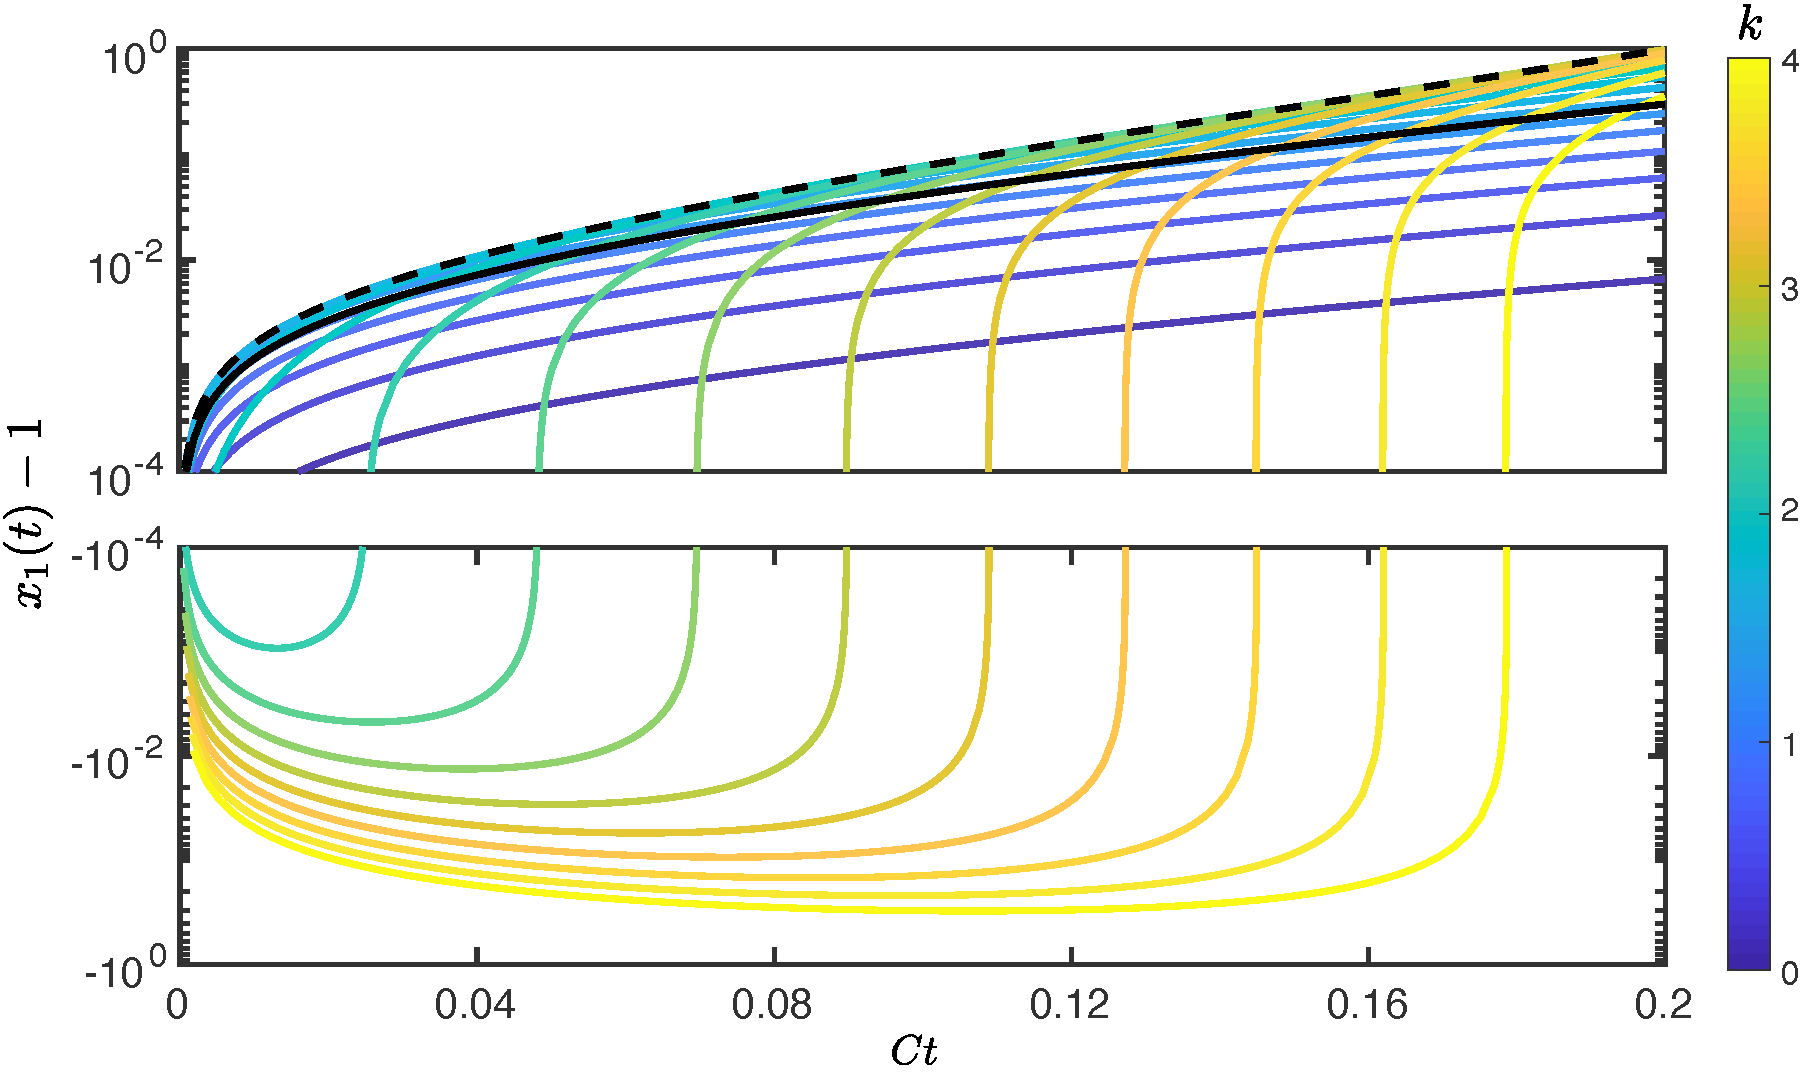
\includegraphics[width = 0.8\textwidth]{overtake_with_asymptotics_and_bvp}
\caption{Growth of the amplitude of the mode of wavenumber $k$ as a function of time as calculated from the ODE~\eqref{E:InstabilityChapter:NonZeroCond:Quasistatic:AsymptoticODE}  with $V_0 = 0.2$, and $\nu = 10$, $a = 0.01$. The upper and lower plots corresponds to increase and decrease of the amplitude of modes, respectively. The colour of the curves indicates the wavenumber $k$, as specified by the colour bar. Also plotted are the envelope of these solutions for small deformations (equation~\eqref{E:InstabilityChapter:NonZeroCond:Quasistatic:AsymptoticODE_envelopeSigma}, black dashed line) and the corresponding envelope for the ODE~\eqref{E:InstabilityChapter:NonZeroCond:Quasistatic:InstantaneousSigma} (solid black curve).}
\label{fig:InstabilityChapter:NonZeroCond:QuasistaticOvertake}
\end{figure}

To demonstrate this possibility explicitly, we consider the small deformation approximation of~\eqref{E:InstabilityChapter:NonZeroCond:Quasistatic:InstantaneousSigma}. Using a tilde to denote this approximation, we have
\begin{equation}\label{E:InstabilityChapter:NonZeroCond:Quasistatic:AsymptoticODE}
\frac{1}{\tilde{x}_1}\dd{\tilde{x}_1}{t}  = \frac{\nu^2 V(t)^7}{\aspect}f\left(\frac{k}{k_c(t)}\right).
\end{equation}
The solution to~\eqref{E:InstabilityChapter:NonZeroCond:Quasistatic:AsymptoticODE} with initial condition $\tilde{x}_1(t = 0) = 1$ is
\begin{equation}\label{E:InstabilityChapter:NonZeroCond:Quasistatic:AsymptoticODE_sol}
\tilde{x}_1= \exp\left\{-\frac{k^2}{6C}\left[|\aspect| k^2 \left(V(t)^2 - V_0^2\right) - \frac{|\nu|}{5}\left(V(t)^5 - V_0^5\right)\right]\right\}.
\end{equation}

We plot in Figure~\ref{fig:InstabilityChapter:NonZeroCond:QuasistaticOvertake} the growth of the amplitude $\tilde{x}_1$ given by~\eqref{E:InstabilityChapter:NonZeroCond:Quasistatic:AsymptoticODE_sol} for various $k$ in which this overtaking mechanism can be seen. At early times, the largest modes are those with small wavenumber (dark curves in Figure~\ref{fig:InstabilityChapter:NonZeroCond:QuasistaticOvertake}), and modes with larger wavenumbers (lighter curves in~\ref{fig:InstabilityChapter:NonZeroCond:QuasistaticOvertake}) decay. However, at later times these modes with larger wavenumber enter into the unstable band and so begin to grow. Some of these modes overtake the smaller wavenumber modes, but those solutions with the largest wavenumbers (the lightest curves in Figure~\ref{fig:InstabilityChapter:NonZeroCond:QuasistaticOvertake}) do not spend enough time in the unstable band to be able to overtake the smaller wavenumber modes before the solution ends with $V(t) = 0.4$.

By maximizing the solution~\eqref{E:InstabilityChapter:NonZeroCond:Quasistatic:AsymptoticODE_sol} with respect to wavenumber $k$, we find that the instantaneously largest mode is
\begin{equation}\label{E:InstabilityChapter:NonZeroCond:Quasistatic:AsymptoticODE_envelopeK}
\tilde{k}_{\textsf{max}}(t) = \sqrt{\frac{\nu}{10\aspect}\frac{V(t)^5 - V_0^5}{V(t)^2 - V_0^2}}.
\end{equation}
The maximum displacement
\begin{equation}\label{E:InstabilityChapter:NonZeroCond:Quasistatic:AsymptoticODE_envelopeSigma}  \tilde{A}_{\text{max} }= \tilde{x}_1\left(t; \tilde{k}_{\text{max}}(t)\right) = \exp \left[\frac{\nu^2}{600C}\frac{\left(V(t)^5 - V_0^5\right)^2}{V(t)^2 - V_0^2}\right]
\end{equation}
describes the envelope of the curves in Figure~\ref{fig:InstabilityChapter:NonZeroCond:QuasistaticOvertake}.

We can find the corresponding envelope valid for (quasistatic) deformations of any size (i.e. not reasonably small) by numerically integrating~\eqref{E:InstabilityChapter:NonZeroCond:Quasistatic:InstantaneousSigma} to find $x_1$ for a range of values of $k$. We use the \texttt{ODE15s} routine implemented in \textsc{matlab} to perform this integration; the growth rate $\sigma_{C=0}$ is evaluated at each time step by solving the quasistatic BVP~\eqref{E:InstabilityChapter:SlowCondensation:Periodic:ODEwet}--\eqref{E:InstabilityChapter:SlowCondensation:Periodic:kinematic} numerically (as described in \S\ref{S:InstabilityChapter:NoCond:Numerics}). The envelope for deformation of any size is tighter than the envelope for small deformations as expected (Figure~\ref{fig:InstabilityChapter:NonZeroCond:QuasistaticOvertake}); numerically obtained values of $\sigma_{C=0}$ are smaller than the corresponding asymptotic approximations, which do not account for the in-plane bending penalty, as discussed in \S\ref{S:InstabilityChapter:NoCondensation:SmallDeformations}.

The analysis of this section serves to demonstrate the overtaking mechanism, and is expected to be valid for $C \ll 1$. To go beyond these results and describe the effect of non-zero condensation rate on mode selection for a general $C$, we must consider the equations describing perturbations from a time-dependent base state, to which we turn now.


\subsection{Periodic perturbations}
To analyze the linear stability of a time-dependent base state to periodic in-plane perturbations, we substitute the ansatz
\begin{align}
h &= h_0(x,t) + \epsilon h_1(x,t)\exp(iky), \\
 p &= p_0(x,t) +\epsilon p_1(x,t) \exp(iky), \\
  x_m &= x_0(t) +\epsilon x_1(t)\exp(iky),
\end{align}
where $\epsilon \ll 1$ is arbitrary, into the model equations~\eqref{E:InstabilityChapter:Modelling:NonDim:PDE1}--\eqref{E:InstabilityChapter:Modelling:NonDim:Kinematic}. Here $h_0, p_0, x_0$ satisfy the base-state equations~\eqref{E:InstabilityChapter:BaseState:FlatInterface:PDEwet}--\eqref{E:InstabilityChapter:BaseState:FlatInterface:kinematicbc}. Linearizing in $\epsilon$ results in a system of spatially one dimensional PDEs:
\begin{align}
\ddp{h_1}{t} &= \frac{1}{3|\nu|} \left[\ddp{}{x}\left(h_0^3 \ddp{p_1}{x} + 3h_0^2 \ddp{p_0}{x}H_1\right)- k^2 h_0^3 p_1\right] & &0 < x < x_0(t), \label{E:InstabilityChapter:WithCondensation:LinearizedEquations:PDEs1}\\
p_1&=0 & & x_0(t) < x < 1.\label{E:InstabilityChapter:WithCondensation:LinearizedEquations:PDEs2}\\
p_1 &= \ddp{^4 h_1}{x^4} - 2k^2 \ddp{^2 h_1}{x^2} + k^4 h_1 & & 0 < x < 1.\label{E:InstabilityChapter:WithCondensation:LinearizedEquations:Pressure2Shape}
\end{align}
The PDEs~\eqref{E:InstabilityChapter:WithCondensation:LinearizedEquations:PDEs1}--\eqref{E:InstabilityChapter:WithCondensation:LinearizedEquations:Pressure2Shape} are subject to the boundary and continuity conditions
\begin{align}
h_1 &= 0 = \ddp{h_1}{x} = \ddp{p_1}{x} = 0 & &\text{at}~x = 0,\label{E:InstabilityChapter:WithCondensation:LinearizedEquations:bc_x=0}\\
p_1 + x_1 \ddp{p_0}{x} &=\frac{\nu}{\h_0^2}\left(x_1\dd{h_0}{x} + h_1\right) + \nu \aspect  k^2 x_1, & &\text{at}~x = x_0.\label{E:InstabilityChapter:WithCondensation:LinearizedEquations:PressureBC}\\
\ddp{^2 h_1}{x^2} - \eta k^2 h_1 &= 0 = \ddp{^3 h_1}{x^2} - (2-\eta) k^2 h_1 & & \text{at}~x = 1.\label{E:InstabilityChapter:WithCondensation:LinearizedEquations:bc_x=1}
\end{align}
\begin{equation}\label{E:InstabilityChapter:WithCondensation:LinearizedEquations:JumpConditions}
\left[h_1\right]_{x_0^-}^{x_0^+} =  \left[\dd{h_1}{\x}\right]_{x_0^-}^{x_0^+} =   \left[\dd{^2h_1}{\x^2}\right]_{x_0^-}^{x_0^+} =  0, \qquad   \left[\dd{^3h_1}{\x^3}\right]_{x_0^-}^{x_0^+}  = \frac{\nu x_1}{h_0(x_0,t)}.
\end{equation}
The perturbation to the meniscus position evolves according to
\begin{equation}\label{E:InstabilityChapter:WithCondensation:LinearizedEquations:kinematic}
\dd{x_1}{t} =-\frac{1}{3|\nu|}\left.\left[ h_0^2 \ddp{p_1}{x} + x_1 \ddp{}{x}\left(h_0^2 \ddp{p_0}{x} \right) + 2 h_0 \ddp{p_0}{x} h_1 \right]\right|_{x = x_0}.
\end{equation}


\subsection{Numerical solutions}
In this section, we describe numerical solutions of the system of linear PDEs~\eqref{E:InstabilityChapter:WithCondensation:LinearizedEquations:PDEs1}--\eqref{E:InstabilityChapter:WithCondensation:LinearizedEquations:kinematic}. These equations are solved simultaneously alongside equations~\eqref{E:InstabilityChapter:BaseState:FlatInterface:PDEwet}--\eqref{E:InstabilityChapter:BaseState:FlatInterface:kinematicbc} describing the base state shape $h_0$, pressure $p_0$ and meniscus position $x_0$. Full details of the numerical scheme are contained in Appendix~\ref{A:Chapter6:Numerics}, but we point in particular to our choice of initial conditions; we anticipate that, as in the zero-condensation case, there are two branches of solutions, one of which has very high decay rates for all $k$ and one of which displays positive growth rates for sufficiently small $k$. To guide our numerics onto the branch displaying positive growth rates, we take the solution to the zero-condensation BVP~\eqref{E:InstabilityChapter:SlowCondensation:Periodic:ODEwet}--\eqref{E:InstabilityChapter:SlowCondensation:Periodic:kinematic} with $V = V_0$ that is on the `correct' branch to be the initial condition on $h_1$ and $p_1$ (with $x_1(0) = 1$ without loss of generality).

\subsubsection{Results}

\begin{figure}[t]
\centering
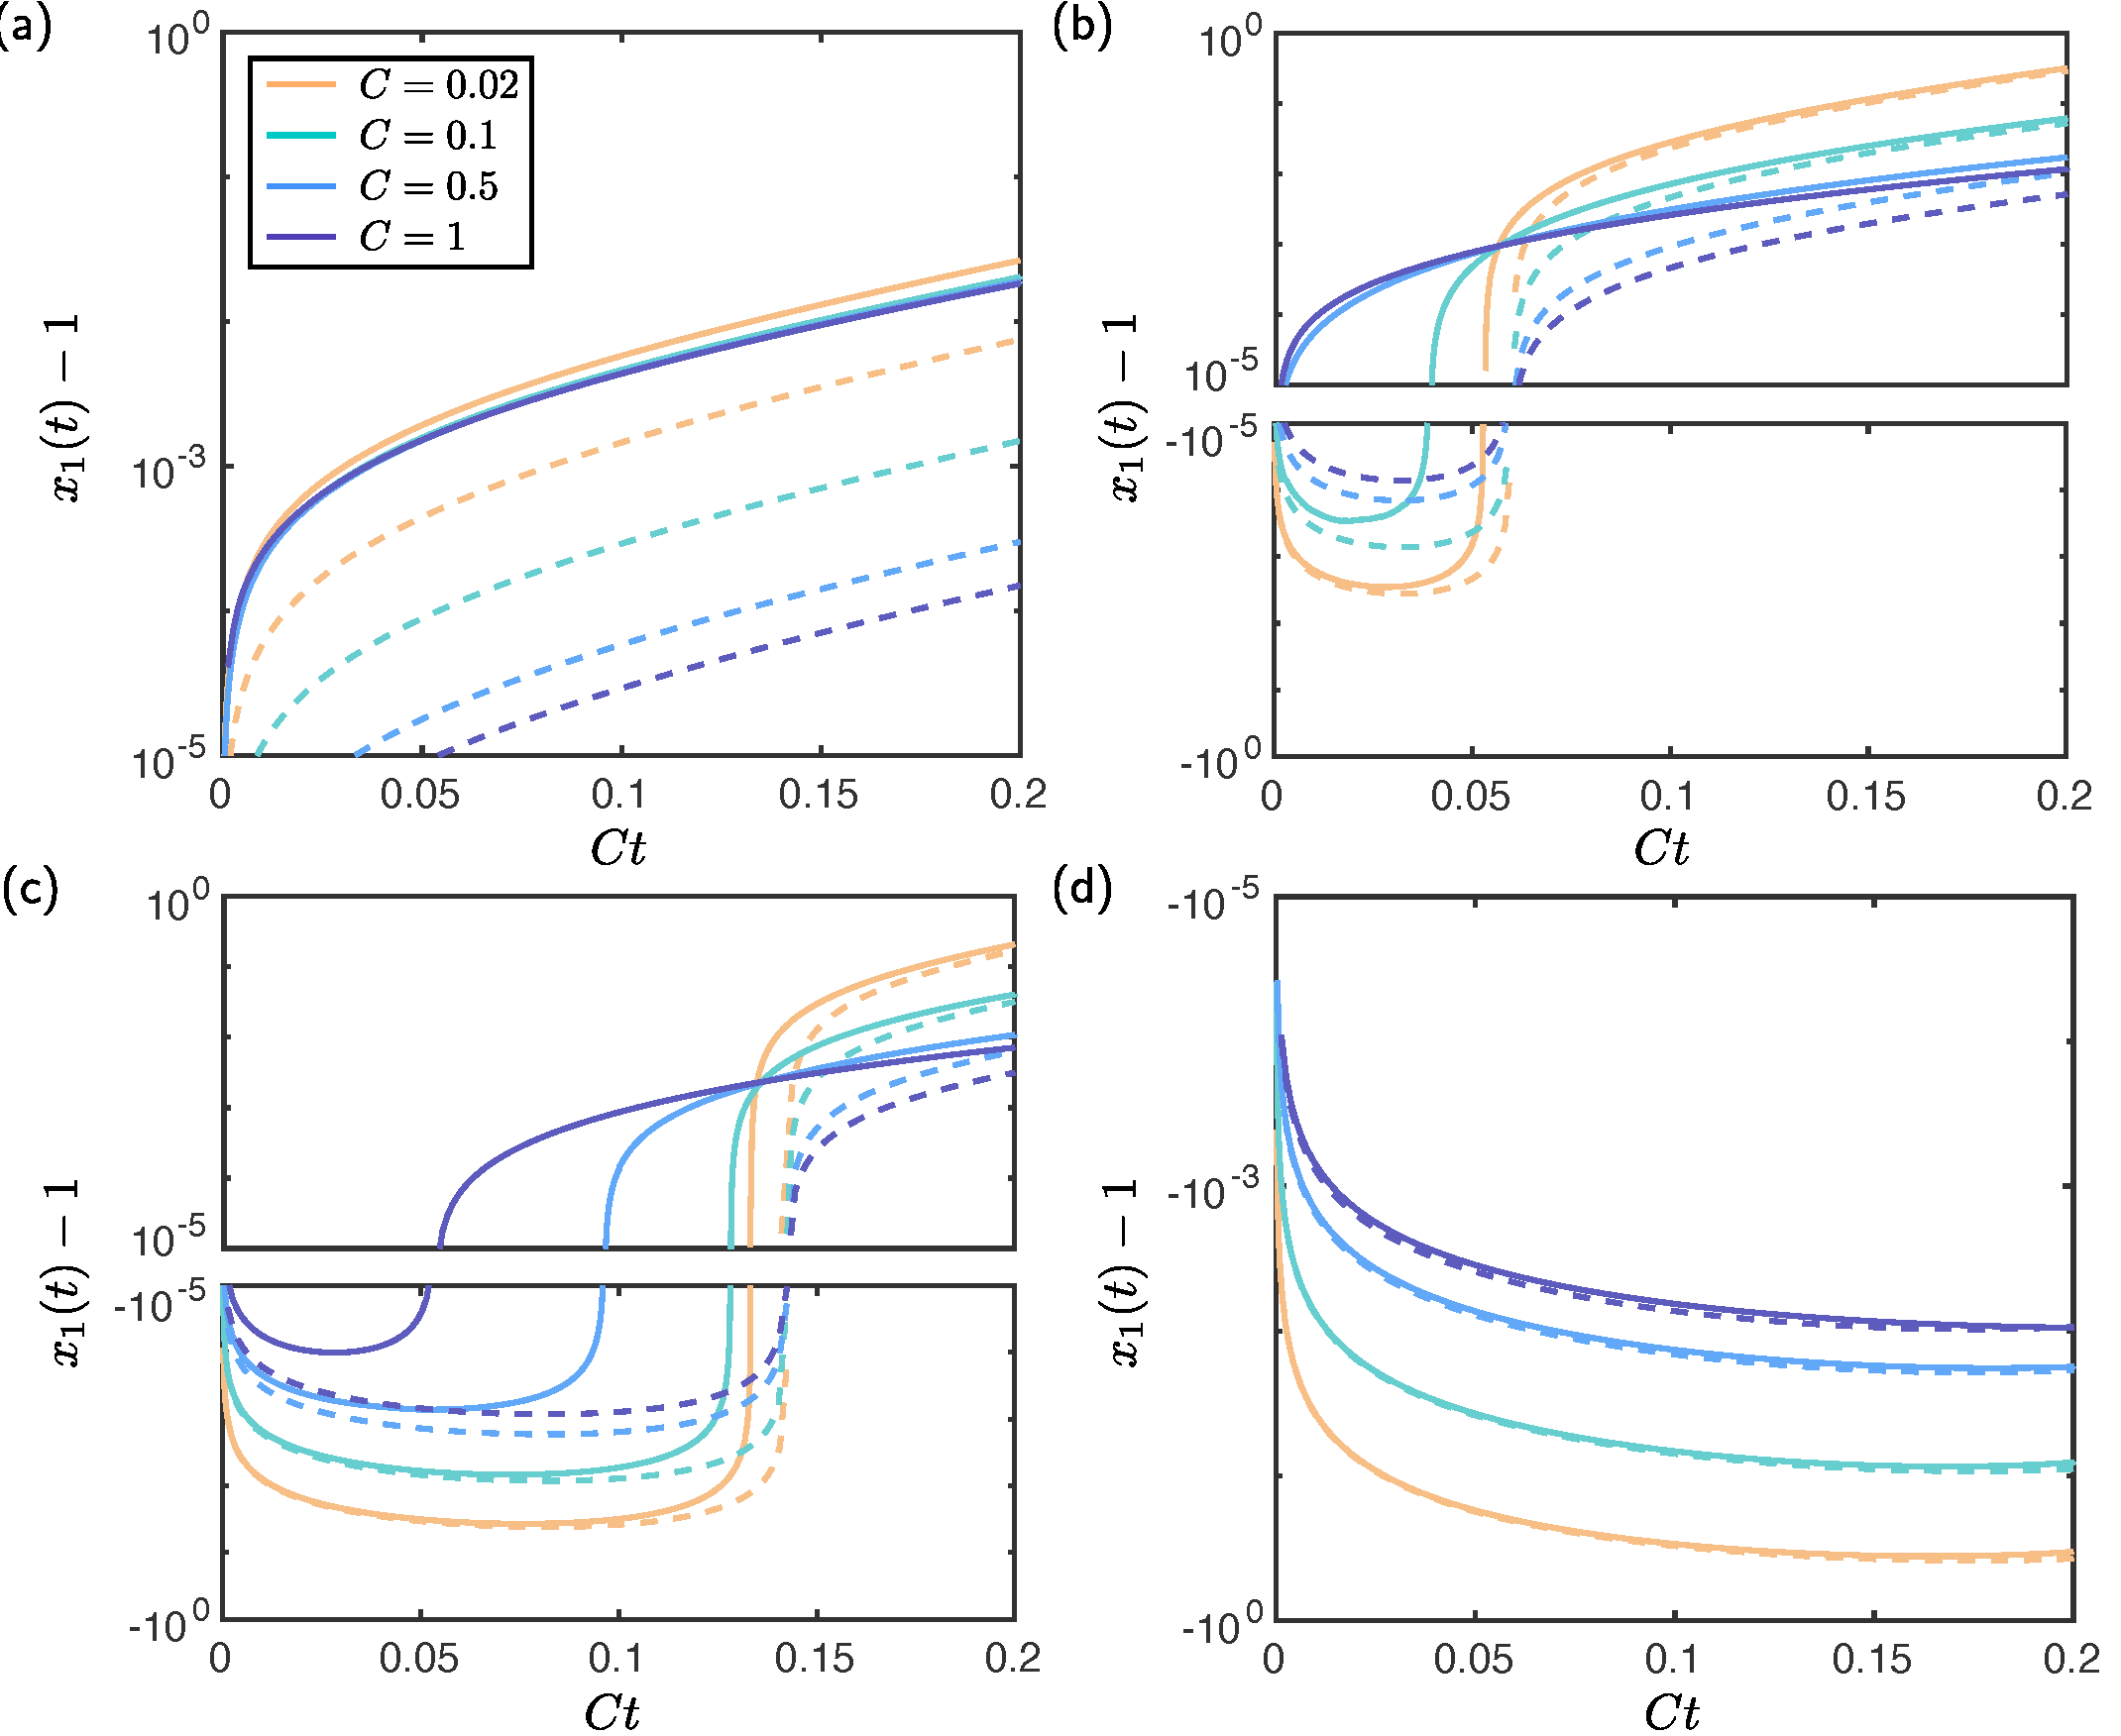
\includegraphics[width = 0.9\textwidth]{v2_full_numerics_traces}
\caption{Numerically obtained displacements, $x_1(t) -1$, of a perturbation to the meniscus position with wavenumber $k$. Data are shown for various condensation rates $C$ (see legend in (a)) and $\nu = 10$, $\aspect = 0.01$, $V_0 = 0.2$. The three plots correspond to  different wavenumbers as follows: (a) $k = 0.2$, (b) $k = 2.1$, (c) $k = 2.6$, and (c) $k = 3.9$. Each trajectory is accompanied by a dashed curve indicating the corresponding quasistatic behaviour, obtained by solving~\eqref{E:InstabilityChapter:NonZeroCond:Quasistatic:InstantaneousSigma} numerically with a linear volume increase, $V(t) = V_0 + Ct$.}
\label{fig:InstabilityChapter:TimeDepBaseState:FullNumericsTraces}
\end{figure}

\begin{figure}[t!]
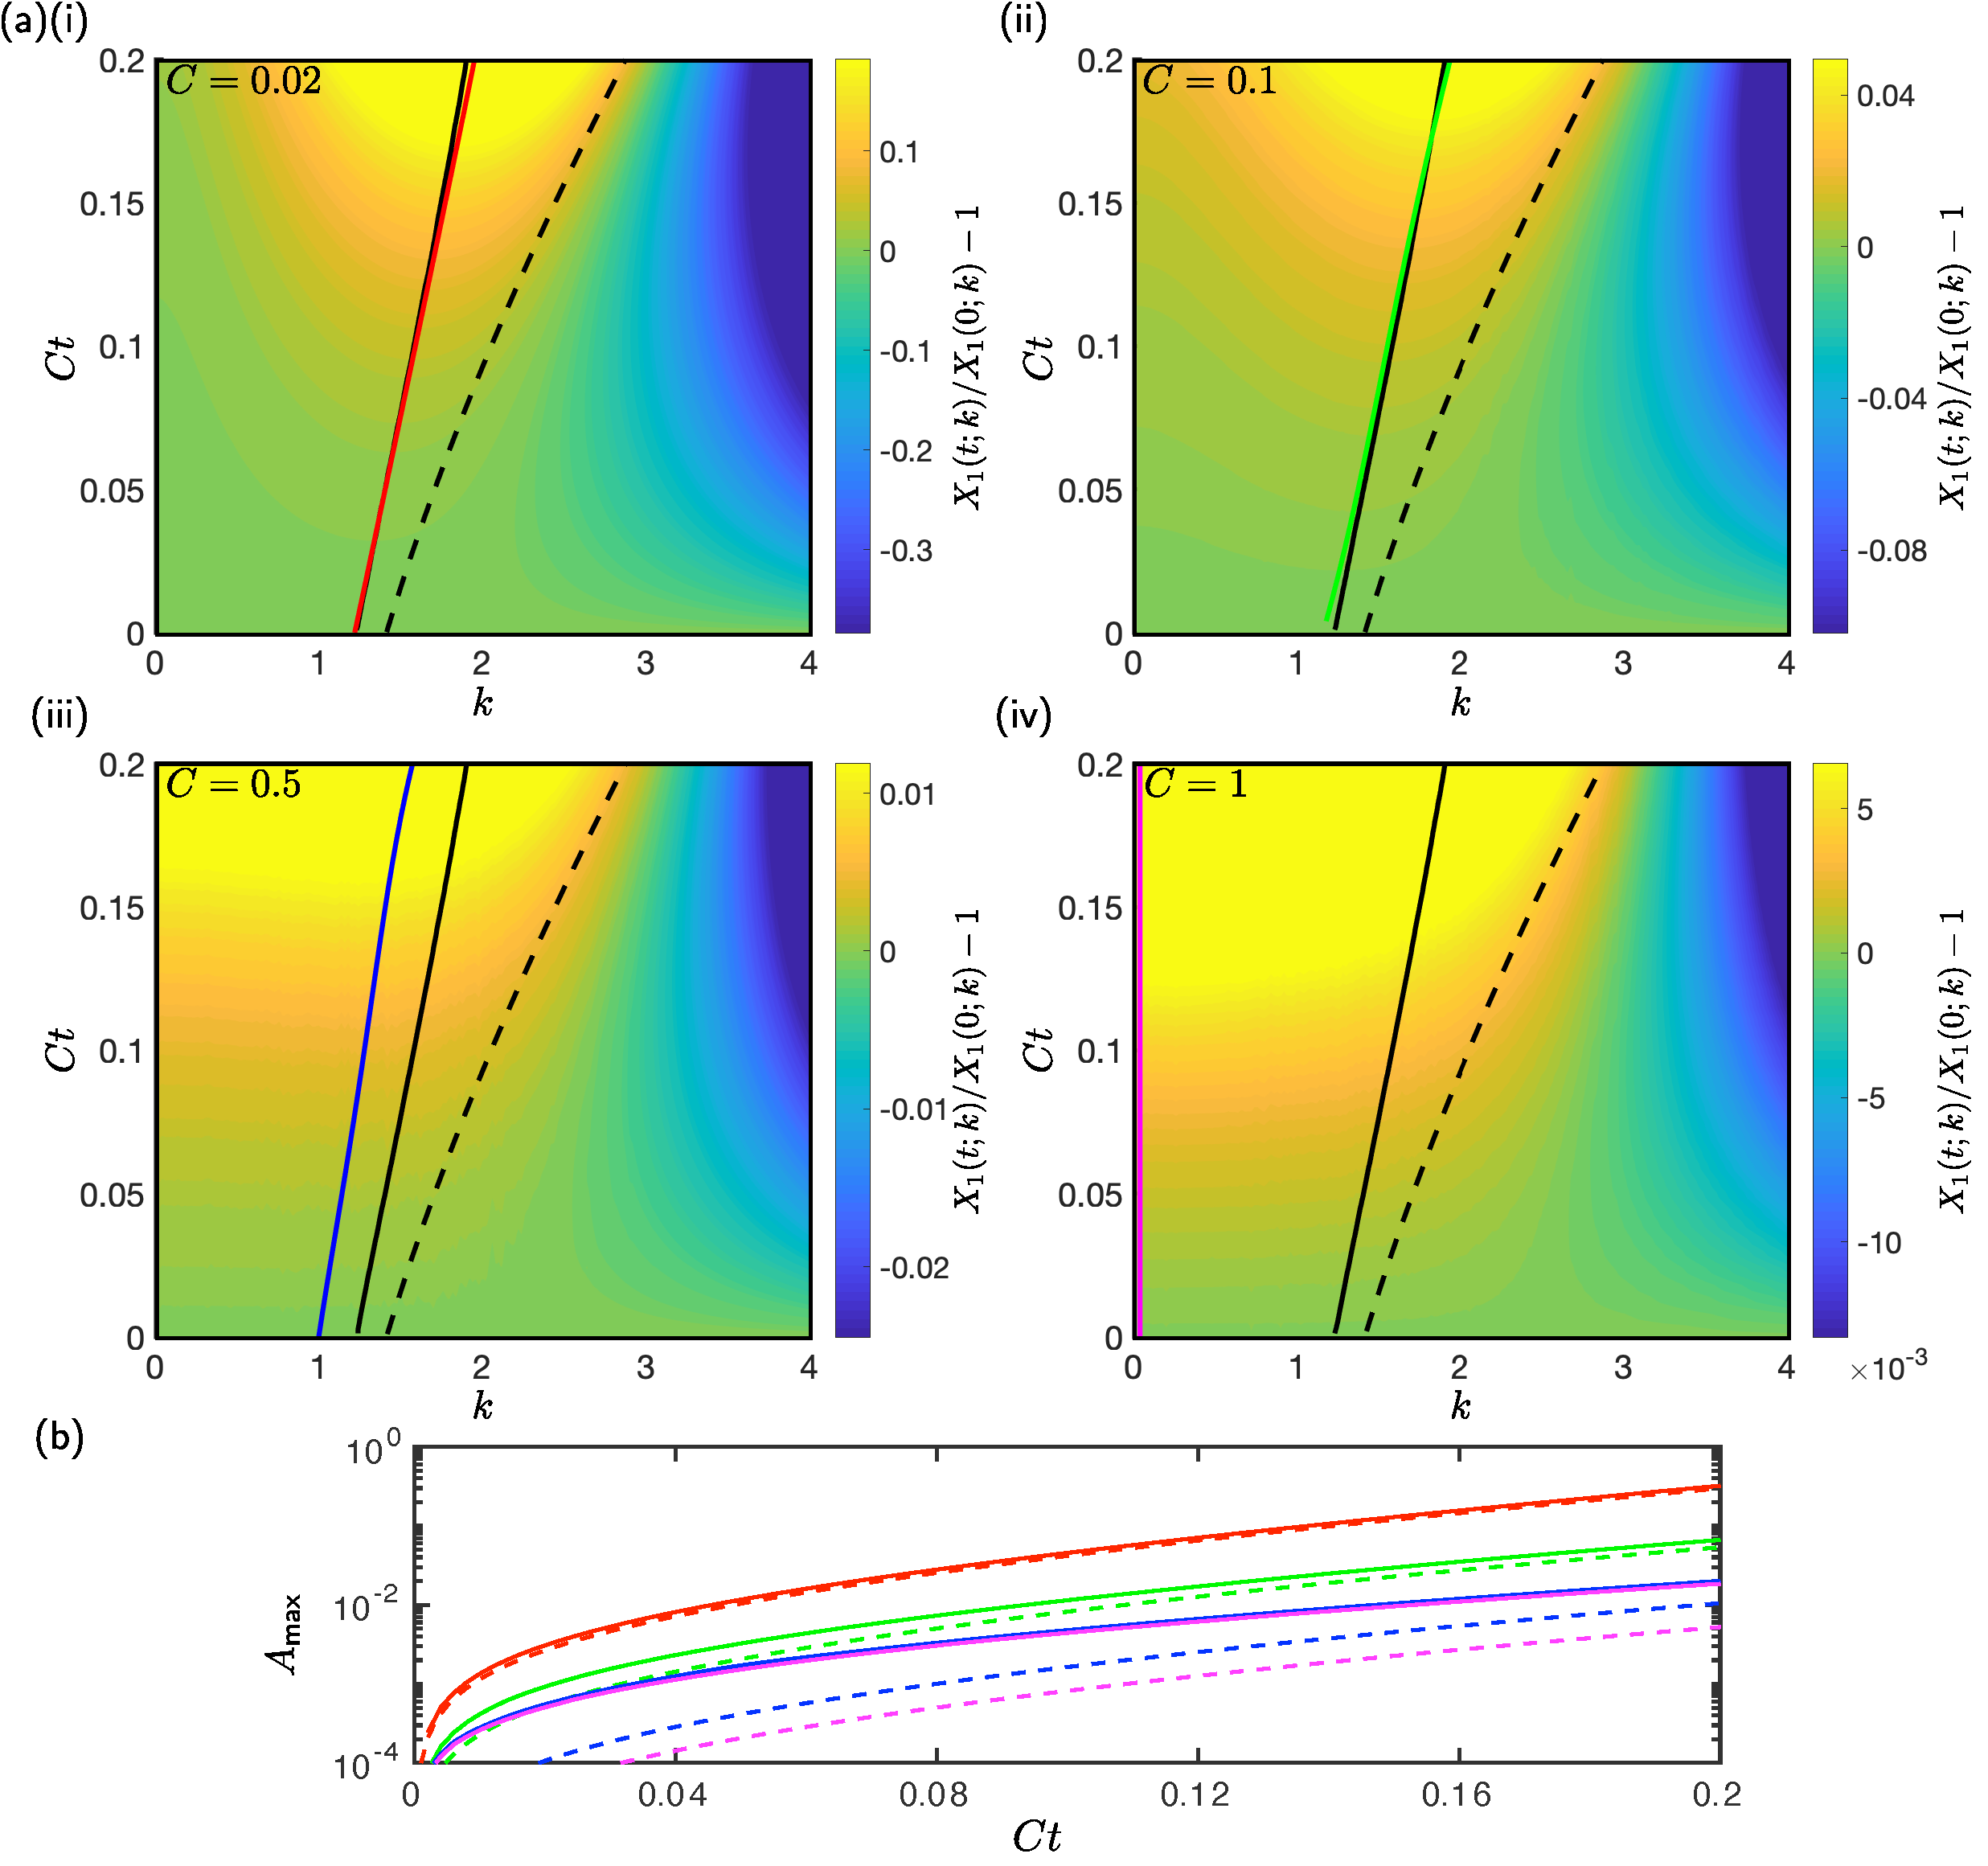
\includegraphics[width = 0.95\textwidth]{contour_plots_various_C}
\caption{Contour plots of mode decay/growth $x_1(t)- 1$: the colour along a vertical line through $k = k_0$ describes the evolution of the perturbation with wavenumber $k_0$ according to the colourbar (note that each colourbar is different, and the colours are saturated to ensure that $0$ has same colour in each plot). The coloured curve (red in (i), green in (ii), blue in (iii), and pink in (iv)) in each plot indicates $k_{\text{max}}$, the mode that has grown the most at each instant of time. The black solid curve indicates the prediction of the quasistatic theory, and the black dashed curve indicates the prediction of the quasistatic theory for small deformations. Results are shown for four different condensation rates are shown as indicated in the top left corner of each plot. (b) Instantaneous maximal displacement, $A_{\text{max}}$ for each of the contour plots in (a). The colours corresponds to those in (a). Also plotted as dashed lines are the corresponding quasistatic approximations to $A_{\text{max}}$.}\label{fig:InstabilityChapter:TimeDepBaseState:contours_k_t_space}
\end{figure}

In Figure~\ref{fig:InstabilityChapter:TimeDepBaseState:FullNumericsTraces} we show the growth of numerically obtained amplitudes $x_1$ for different wavenumbers $k$ and condensation rates $C$.  There are three main qualitative similarities with the quasistatic case described in \S\ref{S:InstabilityChapter:WithCondensation:FrozenTime}. Firstly, modes with small wavenumbers initially grow, and while their growth rate increases, it does so more slowly as time progress (Figure~\ref{fig:InstabilityChapter:TimeDepBaseState:FullNumericsTraces}(a)). Secondly, modes that initially decay start to grow at a finite time and may overtake smaller wavenumber modes (Figure~\ref{fig:InstabilityChapter:TimeDepBaseState:FullNumericsTraces}(b),(c)). Finally, modes with large wavenumbers do not spend enough time in the unstable band to be able to overtake smaller wavenumber modes during the simulation period (Figure~\ref{fig:InstabilityChapter:TimeDepBaseState:FullNumericsTraces}(d)). These observations can be seen for a broader range of wavenumbers $k$ in the contour plots of displacement in Figure~\ref{fig:InstabilityChapter:TimeDepBaseState:contours_k_t_space}, which are generated by numerically solving the equations~\eqref{E:InstabilityChapter:WithCondensation:LinearizedEquations:PDEs1}--\eqref{E:InstabilityChapter:WithCondensation:LinearizedEquations:kinematic} for 200 values of $k$ between $k = 0.02$ and $k = 4$.

However, there are two key differences between the numerical solutions to~\eqref{E:InstabilityChapter:WithCondensation:LinearizedEquations:PDEs1}--\eqref{E:InstabilityChapter:WithCondensation:LinearizedEquations:kinematic} and the quasistatic case of \S\ref{S:InstabilityChapter:WithCondensation:FrozenTime}. Firstly, condensation driven dynamics in the base state enhance the growth rate of perturbations, indicated by the fact that the displacement in numerical solutions is always larger than the corresponding quasistatic approximation. Secondly, the dynamics lengthen the band of unstable modes; in particular, some modes, that initially decay under the quasistatic approximation, grow at early times in the full numerics (compare, for example the $C =0.5$ and $C = 1$ curves in Figure~\ref{fig:InstabilityChapter:TimeDepBaseState:FullNumericsTraces}(b) with the corresponding quasistatic results). These two effects are more pronounced for the largest values of the condensation rate, $C$, as expected.

%how does different wavenumbers change this picture
 At small wavenumbers (Figure~\ref{fig:InstabilityChapter:TimeDepBaseState:FullNumericsTraces}(a)), the numerical solutions (plotted against $Ct$) are almost indistinguishable, suggesting that the growth of the perturbation is controlled primarily by dynamic effects in the base state in this case.
However, at relatively large wavenumbers (Figure~\ref{fig:InstabilityChapter:TimeDepBaseState:FullNumericsTraces}(c)), results barely deviate from the quasistatic prediction, suggesting that the competing-curvature mechanism with a time-dependent volume primarily controls the dynamics, in this case.


The mode with the largest amplitude, denoted $k_{\text{max}}(t)$, and its associated amplitude $A_{\text{max}}(t)$ are time dependent (Figure~\ref{fig:InstabilityChapter:TimeDepBaseState:contours_k_t_space}).
As expected, when the condensation is slow, $k_{\text{max}}$ and $A_{\text{max}}$ are indistinguishable from the quasi-static result (Figure~\ref{fig:InstabilityChapter:TimeDepBaseState:contours_k_t_space}(a)(i)--(ii)). For intermediate condensation rates (Figure~\ref{fig:InstabilityChapter:TimeDepBaseState:contours_k_t_space}(a)(iii)), $k_{\text{max}}(t)$ is shifted towards lower wavenumbers, and the amplitude $A_{\text{max}}$ is enhanced, indicating that condensation driven dynamics of the base state tend to preferentially enhance smaller wavenumber (longer wavelength) modes. (Note that $A_{\text{max}}$ is lower for higher condensation rates when plotted against $Ct$, as in Figure~\ref{fig:InstabilityChapter:TimeDepBaseState:contours_k_t_space}(b), simply because modes have less time to grow -- however, they do show the biggest derivation from the quasistatic theory.) Finally, when condensation is fast, the base state dynamics dominate over the competing curvature instability  -- the mode with the longest wavelength has the largest amplitude (the pink curve in (Figure~\ref{fig:InstabilityChapter:TimeDepBaseState:contours_k_t_space}(a)(iv) corresponds to $k = 0.02$, the smallest wavenumber used to generate the contour plots). For high condensation rates, the maximum amplitude is significantly larger than the corresponding quasistatic prediction  (Figure~\ref{fig:InstabilityChapter:TimeDepBaseState:contours_k_t_space}(b)).

Intuitively, the results described in this section make sense: when liquid is being added to the configuration, the base state is advancing with a flat interface (an infinitely long wavelength), and  those modes which are most coherent (i.e.~have a small wavenumber) will be amplified preferentially.

\section{Summary}
In this Chapter, we set out to understand the periodic pattern that is observed in experiments in which liquid condenses into deformable microchannels. In doing so, we identified a novel instability mechanism that is driven by a competition between interfacial curvatures in the liquid and mediated by the elasticity of the channel in response to liquid pressure. Unlike the similar Al-Housseiny instability, driven by competing interfacial curvatures in liquid confined to a rigid channel, this bendo-capillary instability is theoretically possible in the same channel for both wetting and non-wetting liquids.

We studied this mechanism in detail by considering a simple system that may be susceptible to the instability. For simplicity, we assumed a single meniscus and walls that extend infinitely in the in-plane direction.

We first considered the case of zero condensation, $C = 0$. By performing a linear stability analysis of its equilibrium configurations, we identified that the system is unstable to perturbations of a sufficiently small wavenumber. The linearized equations elucidate the two main ways that the elastic case differs from the rigid (Al-Housseiny) case in two important ways: the bulk channel elasticity is set by the liquid pressure, and the channel responds to the perturbation in a way that tends to enhance the difference between the in-plane and transverse curvatures, increasing the range of unstable wavenumbers. The growth rate of the fastest growing mode is highly sensitive to the amount of liquid within the channel (parametrized by the cross-sectional volume $V$); in particular, we identified that the growth rate $\sigma \sim V^7$ in the case of small deformations and negligible in-plane bending.

In the final section, we analyzed how a non-zero condensation rate affects the mode selection problem. A non-zero condensation rate introduces two variations to the elastocapillary competing-curvature mechanism:  the problem now has a time-dependent volume, and the potential for condensation driven dynamics in the (time-dependent) base state. Numerical solutions of the equations linearized about the base state demonstrated how the modes that initially grow can be overtaken by initially decaying modes, ultimately reaching the non-linear regime earlier. This overtaking behaviour was also predicted analytically with a quasistatic approximation, in which the condensation rate enters via the liquid volume only. Finally, we saw how condensation driven dynamics in the base state result in faster growth of perturbations compared to the quasistatic case, and that modes with smaller wavenumbers are enhanced preferentially.

Ultimately, we expect that the pattern observed at late times will correspond to the mode that is first to reach the non-linear regime, and so the instability refinement we observed will not continue indefinitely. In this sense, the results of the mode selection problem are not able to predict the wavelength that would be observed in practice, but should give a reasonable order of magnitude estimate. In the condensation experiments which originally motivated this study, condensation is very slow ($C \approx 10^{-5}$), and thus condensation driven base state dynamics are unimportant. The quasi-static scaling for the largest wavenumber derived in \S\ref{S:InstabilityChapter:Scaling} should therefore give a order of magnitude estimate for a model prediction of experimentally observed wavelength. Using values from~\cite{Seemann2011JPhysCondMat}, we find that $\nu \approx -12$ and $\aspect \approx -0.38$ in these experiments; the wavelength of approximately $200~\si{\micro \meter}$ that is observed experimentally (see Figure~\ref{fig:InstabilityChapter:Intro:ExptSnapshots}) agrees in its order of magnitude with the scaling result~\eqref{E:InstabilityChapter:Scaling:CriticalWavenumber}, which predicts a wavelength of $370~\si{\micro \meter}$ when the channel is half full, $V = 0.5$. (Note that smaller values of $V$ result in predictions of longer wavelengths, but for $V \approx \mathcal{O}(1)$, these are of the correct order of magnitude; for example with $V = 0.1$, the scaling argument predicts a wavelength of $4~\si{\milli \meter}$.) A more detailed model of the condensation experiments requires consideration of the interaction between neighbouring channels, which appear to undergo the instability simultaneously; this provides motivation for the next chapter, in which we study the interaction between neighbouring channels, each of which would undergo bendotaxis in isolation.

\begin{subappendices}
%\addcontentsline{toc}{section}{Appendices}
\renewcommand{\thesection}{\Alph{section}}
%\appendix
\section{Small deformation asymptotics}\label{A:InstabilityChapter:SmallDeformationAsymptotics}
In this appendix, we describe an asymptotic analysis of the equations describing a periodic perturbation to an equilibrium configuration (equations~\eqref{E:InstabilityChapter:SlowCondensation:Periodic:ODEwet}--\eqref{E:InstabilityChapter:SlowCondensation:Periodic:kinematic}) in the limit of small deformations of the equilibrium configuration, $\epsilon = |\nu| V^4 \ll 1$. In particular, we aim to describe the leading order behaviour of the growth rate $\sigma$ of these perturbations. Note that for simplicity, we consider only wetting configurations here ($\nu >0$) but the analysis is largely similar for non-wetting configurations ($\nu < 0$).

\subsection{Governing equations}\label{A:S:SmallDef:GovEq}
Recall from \S\ref{S:InstabilityChapter:BaseState:Equilibria} that, for $\epsilon \ll 1$, the equilibrium configuration has
\begin{equation}\label{A:E:SmallDeformation:Equations:Asymptotic_x0_to_V}
 x_0 = V\left[1 + \frac{\epsilon}{20}  + \mathcal{O}(\epsilon^2)\right],
\end{equation}
\begin{equation}\label{A:E:SmallDeformation:Equations:Asymptotic_channel_shape}
h_e(x) = 1 + \epsilon\psi \left(\frac{x}{V}\right) + \mathcal{O}(\epsilon^2),\qquad \psi(s) = \frac{-1}{8} + \frac{1}{24}\left[4(1-s) - (1-s)^4\right].
\end{equation}

Before we can proceed with an asymptotic expansion, we need to determine the size of the terms in which the wavenumber $k$ appears. We are primarily interested in those wavenumbers in which the destabilizing transverse and stabilizing in-plane curvature contributions (the terms on the right hand side of~\eqref{E:InstabilityChapter:SlowCondensation:Periodic:pressure_bc}) are comparable. We therefore introduce a scaled wavenumber
\begin{equation}\label{E:Chapter6:SmallDeformation:RescaledProblem:Wavenumber}
k = \left(\frac{\nu V^3}{\aspect}\right)^{1/2} \K,
\end{equation}
which is motivated by the scaling for $k$ we obtained in the scaling argument. We anticipate the majority of the bending deformation occurs in the wet region $0 < x < x_0 = V + \mathcal{O}(\epsilon)$, and introduce the rescaled spatial variable $X = x/V$ to reflect this.

After inserting~\eqref{E:Chapter6:SmallDeformation:RescaledProblem:Wavenumber} and the scaled variable $X$ into the BVP~\eqref{E:InstabilityChapter:SlowCondensation:Periodic:ODEwet}--\eqref{E:InstabilityChapter:SlowCondensation:Periodic:kinematic}, the parameter
\begin{equation}\label{AE:InstabilityChapter:SmallDeformation:RescaledProblem:OtherSmallPar}
\param= \frac{\nu V^5}{|\aspect|} \gg \epsilon
\end{equation}
appears naturally. The parameter $\param$ describes the ratio between bending energies in the in-plane and transverse directions (see \S\ref{S:InstabilityChapter:NoCondensation:SmallDeformations}). The requirement that $\param \gg \epsilon$ ensures that our use of lubrication theory is valid.

We consider the behaviour in the limit $\param \to 0$, which corresponds to relatively small in-plane bending deformations, compared to transverse bending deformations. We expect that the majority of the bending of the dry region occurs in the in-plane direction, so for $\param \ll 1$, the bending of the dry region is not significant. 

We also rescale the perturbed channel shape $H$ and pressure $P$ with $\nu V^3$ to reflect the leading order behaviour -- a shearing force of magnitude $\nu$ applied over a length equal to the magnitude of the perturbation (the shear is the third derivative of the channel deformation, which combined with the length rescaling is responsible for the $V^3$).

After inserting~\eqref{A:E:SmallDeformation:Equations:Asymptotic_x0_to_V} and~\eqref{A:E:SmallDeformation:Equations:Asymptotic_channel_shape} into BVP~\eqref{E:InstabilityChapter:SlowCondensation:Periodic:ODEwet}--\eqref{E:InstabilityChapter:SlowCondensation:Periodic:kinematic}, the problem for
\begin{equation}
G(X) = \frac{H(X)}{\nu V^3}, \qquad Q(X) = \frac{P(X)}{\nu V^3}
\end{equation}
and $\sigma$ reads, correct to $\mathcal{O}\left(\epsilon^2\right)$:
\begin{align}
3\epsilon V^2 \sigma G &= \left(1 + 2\epsilon \psi\right)\left[\epsilon\dd{\psi}{X} \dd{Q}{X} + \left(1 + \epsilon \psi\right)\left(\dd{^2 Q}{X^2} -\param K^2 Q\right)\right] & &0 < X < 1,\label{A:E:Chapter6:SmallDef:BVP:ODEwet}\\
0 &= Q & &1 < X < \frac{1}{V},\label{A:E:Chapter6:SmallDef:BVP:ODEdry}\\
Q &= \dd{^4 G}{X^4} - 2\param K^2 \dd{^2 G}{X^2} +\param K^4 G & &0 < X<\frac{1}{V},\label{A:E:Chapter6:state_BVP:pressure2shape}
\end{align}
with boundary conditions
\begin{align}
G &= 0 = \dd{G}{X} = \dd{Q}{X} & &\text{at}~X = 0,\label{A:E:Chapter6:SmallDef:BVP:BC_at_0}\\
Q + \frac{\epsilon V}{20}\ddp{Q}{X} &= \epsilon\left(\dd{\psi}{X} + G + K^2\right)  & &\text{at}~X= 1,\label{A:E:Chapter6:SmallDef:BVP:pressure_bc}\\
\dd{^2 G}{X^2} -\param \poisson K^2 G &= 0 = \dd{^3 G}{X^3} - (2-\poisson)\param K^2 \dd{G}{X} & &\text{at}~X = \frac{1}{V},\label{A:E:Chapter6:SmallDef:BVP:BC_at_1}
\end{align}
\begin{align}\label{A:E:Chapter6:SmallDef:BVP:jump_conds}
\left[G\right]_-^+= \left[\dd{G}{x}\right]_-^+ = \left[\dd{^2G}{X^2} + \frac{\epsilon V}{20}\dd{^3 G}{X^3}\right]_-^+&= 0, \\
\left[\dd{^3 G}{X^3} + \frac{\epsilon V}{20}\dd{^4 G}{X^4}\right]_-^+ &= 1 - \epsilon \psi(1).
\end{align}
Here the jump applies across the (unperturbed) contact line $X = 1$.The growth rate $\sigma$ satisfies
\begin{equation}\label{A:E:Chapter6:SmallDef:BVP:kinematic}
3V^2\sigma = -\left[1 + 2\epsilon \psi(1)\right]\left[\dd{Q}{X} + \frac{\epsilon V}{20}\dd{^2 Q}{X^2}\right]_{X = 1}.
\end{equation}

\subsection{Bivariate expansion}
We analyse the asymptotic structure of the rescaled problem~\eqref{A:E:Chapter6:SmallDef:BVP:ODEwet}--\eqref{A:E:Chapter6:SmallDef:BVP:kinematic} by posing the bivariate asymptotic expansion
\begin{align}
G &=  G_{0,0} + \param G_{1,0} + \epsilon G_{0,1} +  \param^2 G_{2,0} + \param \epsilon G_{1,1} + \epsilon^2 G_{0,2} + \dots,\label{A:E:Chapter6:SmallDeformation:Expansion:ExpansionH} \\
Q &=  Q_{0,0} + \param Q_{1,0} + \epsilon Q_{0,1} +  \param^2 Q_{2,0} + \param \epsilon Q_{1,1} + \epsilon^2 Q_{0,2} + \dots,\label{A:E:Chapter6:SmallDeformation:Expansion:ExpansionP} \\
\sigma &= \sigma_{0,0} + \param \sigma_{1,0} + \epsilon \sigma_{0,1} +  \param^2 \sigma_{2,0} + \param \epsilon \sigma_{1,1} + \epsilon^2 \sigma_{0,2} + \dots. \label{A:E:Chapter6:SmallDeformation:Expansion:ExpansionSigma}
\end{align}
The particular hierarchy of problems that emerges depends on the relative sizes of $\epsilon$ and $\param \gg \epsilon$. Clearly, if $\epsilon \ll \param^2$, terms like $G_{2,0}$ will dominate $G_{0,1}$ while if $\param^2 \ll \epsilon$ it will be the other way around. We therefore consider the distinguished limit $\epsilon \sim \param^2$, writing $\epsilon = \beta \param^2$ with $\beta \sim \mathcal{O}(1)$. (In any case, the first and leading order problems are independent of the precise details of the relative sizes of $\epsilon$ and $\param \gg \epsilon$.)

We therefore rewrite the expansion as
\begin{align}
G &= G_0 + \param G_1 + \param^2 G_2 + \param^3 G_3 + \mathcal{O}\left(\param^4\right),\\
Q &= Q_0 + \param Q_1 + \param^2 Q_2 + \param^3 Q_3 + \mathcal{O}\left(\param^4\right),\label{A:E:SmallDef:Expansion:ExpansionQ}\\
\sigma &= \sigma_0 + \param \sigma_1 + \param^2 \sigma_2 + \param^3 \sigma_3 + \mathcal{O}\left(\param^4\right).
\end{align}
We do not include any terms that are $\mathcal{O}\left(\param^4\right) = \mathcal{O}\left(\epsilon^2\right)$ because the rescaled problem~\eqref{A:E:Chapter6:SmallDef:BVP:ODEwet}--\eqref{A:E:Chapter6:SmallDef:BVP:kinematic} is only correct to $\mathcal{O}\left(\epsilon^2\right)$.

\subsubsection{Leading and first order problem}
The leading order problem is given by
\begin{align}
0&= \dd{^2Q_0}{X^2} & &0 < X<1,\label{A:E:Chapter6:SmallDef:Expansion:0thOrder:ODEwet}\\
0&= Q_0  & &1 < X< \frac{1}{V},\\
Q_0 &= \dd{^4 G_0}{X^4} & & 0 < X < \frac{1}{V},
\end{align}
\begin{align}
G_0 &= 0 = \dd{G_0}{X}= \dd{Q_0}{X} & &\text{at}~X = 0,\label{A:E:Chapter6:SmallDef:Expansion:0thOrder:x0bc}\\
Q_0 &=0 & &\text{at}~X = 1,\label{A:E:Chapter6:SmallDef:Expansion:0thOrder:pressurebc}\\
\dd{^2 G_0}{X^2} &=0 = \dd{^3 G_0}{X^3} & &\text{at}~X = \frac{1}{V},
\end{align}
\begin{equation}
\left[G_0\right]_-^+ =0 = \left[\dd{G_0}{X}\right]_-^+ = \left[\dd{^2 G_0}{X^2}\right]_-^+, \quad  \left[\dd{^3 G_0}{X^3}\right]_-^+ = 1
\end{equation}
\begin{equation}\label{A:E:Chapter6:SmallDef:Expansion:0thOrder:kinematic}
3V^2 \sigma_0 = -\left.\dd{Q_0}{X}\right|_{X=1}
\end{equation}
From~\eqref{A:E:Chapter6:SmallDef:Expansion:0thOrder:ODEwet},  the pressure $Q_0$ is a linear function of $X$. However, from~\eqref{A:E:Chapter6:SmallDef:Expansion:0thOrder:x0bc}--\eqref{A:E:Chapter6:SmallDef:Expansion:0thOrder:pressurebc}, this linear function has no slope and passes through zero; we therefore have $Q_0 = 0$, and from~\eqref{A:E:Chapter6:SmallDef:Expansion:0thOrder:kinematic} $\sigma_0 = 0$. The solution to~\eqref{A:E:Chapter6:SmallDef:Expansion:0thOrder:ODEwet}--\eqref{A:E:Chapter6:SmallDef:Expansion:0thOrder:kinematic} for the channel shape is
\begin{equation}\label{A:E:Chapter6:SmallDef:Expansion:0thOrder:shape_sol}
G_0 = \begin{cases}
-\frac{\X^2}{6}\left(3-X\right) & 0 < X < 1,\\
-\frac{1}{6}\left(X-1\right) & 1< X < 1/V.
\end{cases}
\end{equation}

The first order problem is similar. Again, we get no pressure contribution, $Q_1 = 0$ (the equations for $Q_1$ are identical to those for $Q_0$) and thus $\sigma_1 = 0$. The shape contribution $G_1$ is non-trivial, but is not required for the determination of the leading order behaviour for $\sigma$, and we therefore do not state it here. We note, however, that the Poisson's ratio $\poisson$ first appears in this term, highlighting the lower order contribution of the dry regions. (For a balance between $\epsilon$ and $\param$ other than $\epsilon \sim \param^2$, as assumed here, the  statements in this paragraph remain true.)
%%%%%%%%%%%%%%%%%%%%%
%%% First order problem %%%%%%%

%\subsubsection{First order problem}
%Using the solutions \red{ref}, the first order problem is very similar
%\begin{align}
%0&= \ddp{^2 Q_1}{X^2}  & &0 < X<1,\label{A:E:Chapter6:SmallDef:Expansion:1stOrder:ODEwet}\\
%0 &= Q_1 & &1 < X< \frac{1}{V},\\
%Q_1 &= \dd{^4 G_1}{X^4}  - 2K^2 \dd{^2 G_0}{X^2}& & 0 < X < \frac{1}{V},
%\end{align}
%\begin{align}
%G_1 &= 0 = \dd{G_1}{X}= \dd{Q_1}{X} & &\text{at}~X = 0,\\
%Q_1 &=0 & &\text{at}~X = 1,\\
%\dd{^2 G_1}{X^2} - \poisson K^2 G_0 &=0 = \dd{^3 G_1}{X^3} - (2- \poisson )K^2 \dd{G_0}{X}& &\text{at}~X = \frac{1}{V},
%\end{align}
%\begin{equation}
%\left[G_1\right]_-^+ =0 = \left[\dd{G_1}{X}\right]_-^+ = \left[\dd{^2 G_1}{X^2}\right]_-^+ =  \left[\dd{^3 G_1}{X^3}\right]_-^+
%\end{equation}
%\begin{equation}\label{A:E:Chapter6:SmallDef:Expansion:1stOrder:kinematic}
%3V^2 \sigma_1 = -\left.\dd{Q_1}{X}\right|_{X=1}.
%\end{equation}

\subsubsection{Higher order problems}
The  $\mathcal{O}(\param^2)$ problem may be expressed simply be exploiting the  $\mathcal{O}(1)$ and $\mathcal{O}(\param)$ problems. We give only this simplified form here:
\begin{align}
 \dd{^2 Q_2}{X^2}&=0 & &0 < X<1,\\
Q_2 &= 0 & &1 < X< \frac{1}{V},\\
Q_2 &= \dd{^4 G_2}{X^4} - 2K^2\dd{G_1}{X^2}+ K^4 G_0 & & 0 < X < \frac{1}{V},
\end{align}
\begin{align}
G_2 &= 0 = \dd{G_2}{X}= \dd{Q_2}{X} & &\text{at}~X = 0,\\
Q_2 &=G_0+ K^2+ \dd{\psi}{X} & &\text{at}~X = 1,\label{A:E:Chapter6:SmallDef:Expansion:2ndOrder:PressureBC}\\
\dd{^2 G_2}{X^2} - \poisson K^2 G_1 &=0 = \dd{^3 G_0}{X^3}  - (2- \poisson)K^2 \dd{G_1}{X}& &\text{at}~X = \frac{1}{V},
\end{align}
\begin{equation}
\left[G_2\right]_-^+ =0 = \left[\dd{G_2}{X}\right]_-^+ = \left[\dd{^2 G_2}{X^2} + \frac{\beta V}{20}\dd{^3G_0}{X^3}\right]_-^+, = \left[\dd{^3 G_2}{X^3} + \frac{\beta V}{20}\dd{^4 G_0}{X^4}\right]_-^+
\end{equation}
\begin{equation}
3V^2 \sigma_2 = -\left.\dd{Q_2}{X}\right|_{X=1}.
\end{equation}
Crucially, the boundary condition~\eqref{A:E:Chapter6:SmallDef:Expansion:2ndOrder:PressureBC} is inhomogeneous, in contrast to the corresponding boundary condition for the lower order problem. We therefore find the first non-zero pressure term in~\eqref{A:E:SmallDef:Expansion:ExpansionQ} to be
\begin{equation}\label{A:E:Chapter6:SmallDef:Expansion:2ndOrder:solQ2}
Q_2 = \begin{cases}
K^2 - \frac{1}{2} & 0 <X  < 1,\\
0 & 1 < X < 1/V,
\end{cases}
\end{equation}
where we have used $G_0$, from~\eqref{A:E:Chapter6:SmallDef:Expansion:0thOrder:shape_sol}, to obtain $Q_2$. (Note that for a relationship other than $\epsilon\sim \param^2$, the boundary condition~\eqref{A:E:Chapter6:SmallDef:Expansion:2ndOrder:PressureBC} would be unchanged because the shape contributions at higher order all take the same value at $ X= 1$.) This leading order pressure contribution is constant in the liquid and thus again offers no contribution to the growth rate, hence $\sigma_2 = 0$.

To obtain a non-zero term in the expansion for $\sigma$ we must proceed to $\mathcal{O}(\param^3)$, where we find that
\begin{align}
 \dd{^2 Q_3}{X^2} - K^2 Q_2 &= 0 & &0 < X<1,\label{A:E:Chapter6:SmallDef:Expansion:3ndOrder:odewet}\\
Q_3 &= 0 & &1 < X< \frac{1}{V},\\
Q_3 &= \dd{^4 G_3}{X^4} - 2K^2\dd{G_2}{X^2}+ K^4 G_1 & & 0 < X < \frac{1}{V},
\end{align}
\begin{align}
G_3 &= 0 = \dd{G_3}{X}= \dd{Q_3}{X} & &\text{at}~X = 0,\label{A:E:Chapter6:SmallDef:Expansion:3ndOrder:x0bc}\\
Q_3 &=\beta G_1 & &\text{at}~X = 1,\label{A:E:Chapter6:SmallDef:Expansion:3ndOrder:PressureBC}\\
\dd{^2 G_2}{X^2} - \poisson K^2 G_1 &=0 = \dd{^3 G_0}{X^3}  - (2- \poisson)K^2 \dd{G_1}{X}& &\text{at}~X = \frac{1}{V},
\end{align}
\begin{equation}
\left[G_3\right]_-^+ =0 = \left[\dd{G_3}{X}\right]_-^+ = \left[\dd{^2 G_3}{X^2} + \frac{\beta V}{20}\dd{^3G_1}{X^3}\right]_-^+, = \left[\dd{^3 G_3}{X^3} + \frac{\beta V}{20}\dd{^4 G_1}{X^4}\right]_-^+
\end{equation}
\begin{equation}\label{A:E:Chapter6:SmallDef:Expansion:3ndOrder:kinematic}
3V^2 \sigma_3 = -\left.\dd{Q_3}{X}\right|_{X=1}.
\end{equation}
From~\eqref{A:E:Chapter6:SmallDef:Expansion:3ndOrder:odewet} and~\eqref{A:E:Chapter6:SmallDef:Expansion:3ndOrder:x0bc}, we find that
\begin{equation}\label{A:E:Chapter6:SmallDef:Expansion:3ndOrder:solutionQ3}
\dd{Q_3}{X} = K^2 Q_2 X \qquad 0 < X < 1.
\end{equation}
Inserting~\eqref{A:E:Chapter6:SmallDef:Expansion:3ndOrder:solutionQ3} into~\eqref{A:E:Chapter6:SmallDef:Expansion:3ndOrder:kinematic}, and using~\eqref{A:E:Chapter6:SmallDef:Expansion:2ndOrder:solQ2} gives
\begin{equation}\label{A:E:Chapter6:SmallDef:Expansion:3ndOrder:solutionsigma3}
\sigma_3  = -\frac{K^2}{6V^2}\left(2K^2 - 1\right).
\end{equation}
This is the leading order term in the expansion~\eqref{A:E:Chapter6:SmallDeformation:Expansion:ExpansionSigma} for $\sigma$.

Undoing the various variable changes introduced in Appendix~\ref{A:S:SmallDef:GovEq}, the result~\eqref{A:E:Chapter6:SmallDef:Expansion:3ndOrder:solutionsigma3} gives
\begin{equation}\label{AE:InstabilityChapter:SmallDeformation:ThirdOrder:SigmaSolution}
\sigma\sim \frac{\nu^2 V^7}{a}F\left(\frac{k}{k_c}\right)
\end{equation}
where
\begin{equation}\label{AE:InstabilityChapter:SmallDeformation:ThirdOrder:SigmaSolutionParticulars}
F(\xi) = -\frac{\xi^2}{6}\left(2\xi^2 -1\right), \qquad k_c = \left(\frac{\nu V^3}{a}\right)^{1/2}.
\end{equation}
Note that~\eqref{AE:InstabilityChapter:SmallDeformation:ThirdOrder:SigmaSolution} agrees with the scaling argument presented in \S\ref{S:InstabilityChapter:Scaling}.

\section{Details of numerical scheme}\label{A:Chapter6:Numerics}
In this appendix, we give details of the numerical scheme used to solve the system of PDEs and boundary conditions~\eqref{E:InstabilityChapter:BaseState:FlatInterface:PDEwet}--\eqref{E:InstabilityChapter:BaseState:FlatInterface:kinematicbc} and~\eqref{E:InstabilityChapter:WithCondensation:LinearizedEquations:PDEs1}--\eqref{E:InstabilityChapter:WithCondensation:LinearizedEquations:kinematic} for $h_0, h_1, p_0,p_1, x_0, x_1$ that describe both the dynamic evolution of the base state, and the growth of periodic perturbations to it. Note that the equations describing the evolution of $h_0, p_0,x_0$ can be solved without also solving for $h_1, p_1,x_1$ (but not the other way around) so this section also describes the scheme used to numerically solve the PDEs~\eqref{E:InstabilityChapter:BaseState:FlatInterface:PDEwet}--\eqref{E:InstabilityChapter:BaseState:FlatInterface:kinematicbc} for $h_0, p_0,x_0$ in isolation.

\subsection{Isolating the wet region}
We begin by reducing the problem to be solved to one defined only on the wet region, $0 < x < x_0(t)$. This is possible because both the base state channel shape $h_0$, and the perturbation to it, $h_1$, can be expressed analytically in the the dry region ($x_0 < x < 1$) in terms of the channel shape at $x = x_0$.

Explicitly, we integrate~\eqref{E:InstabilityChapter:BaseState:FlatInterface:PDEwet}--\eqref{E:InstabilityChapter:BaseState:FlatInterface:pressure2shape}
and~\eqref{E:InstabilityChapter:WithCondensation:LinearizedEquations:PDEs2}--\eqref{E:InstabilityChapter:WithCondensation:LinearizedEquations:Pressure2Shape} directly to obtain
\begin{align}
h_0 &= C_1 x + C_1 & & x_0(t) < x < 1,\label{E:InstabilityChapter:WithCondensation:Numerics:dry_solution0}\\
h_1 &= (D_1 x + D_2)\exp(kx) + (D_3 x + D_4)\exp(-kx) & & x_0(t) < x < 1,\label{E:InstabilityChapter:WithCondensation:Numerics:dry_solution1}
\end{align}
where the $C_i(t), D_i(t), i = 1,\dots, 4$ are constants of integration.

Inserting~\eqref{E:InstabilityChapter:WithCondensation:Numerics:dry_solution1} into the two boundary conditions~\eqref{E:InstabilityChapter:WithCondensation:LinearizedEquations:bc_x=1} and the four continuity  conditions~\eqref{E:InstabilityChapter:WithCondensation:LinearizedEquations:JumpConditions} allows us to express the $C_i, i = 1,\dots,4$ in terms of the channel shape at $x = x_0$ provided that two constraints on the wall shape of the form
\begin{equation}\label{E:InstabilityChapter:WithCondensation:Numerics:effbc}
\ddp{^3 h_1}{x^3} = \psi_1 \ddp{h_1}{x} + \psi_2 h_1 + \psi_3 x_1, \quad \ddp{^2 h_1}{x^2} = \phi_1 \ddp{h_1}{x} + \phi_2 h_1 + \phi_3 x_1 \quad \text{at}~x  = x_0
\end{equation}
hold. Here $\psi_i, \phi_i, i = 1,2,3$ are (known) functions of $k, \eta, x_0,$ and $\nu$. Equations~\eqref{E:InstabilityChapter:WithCondensation:Numerics:effbc} can be thought of as effective boundary conditions, which parametrise the effect of the dry region on the wet region.

The same procedure applied to the base state results in effective boundary conditions
\begin{equation}\label{E:InstabilityChapter:WithCondensation:Numerics:effbc_base_state}
\ddp{^3 h_0}{x^3} = 0= \ddp{^2 h_1}{x^2} \quad\text{at}~x  = x_0.
\end{equation}

With~\eqref{E:InstabilityChapter:WithCondensation:Numerics:effbc} and~\eqref{E:InstabilityChapter:WithCondensation:Numerics:effbc_base_state}, we have a complete system of equations for $h_0$, $h_1$,  $p_0$, $p_1$, $x_0$, and $x_1$ that involves only the drop region. These are the four PDEs~\eqref{E:InstabilityChapter:BaseState:FlatInterface:PDEwet}, \eqref{E:InstabilityChapter:BaseState:FlatInterface:pressure2shape}, \eqref{E:InstabilityChapter:WithCondensation:LinearizedEquations:PDEs1}, \eqref{E:InstabilityChapter:WithCondensation:LinearizedEquations:Pressure2Shape}, the boundary conditions~\eqref{E:InstabilityChapter:BaseState:FlatInterface:bc0}--\eqref{E:InstabilityChapter:BaseState:FlatInterface:jumpbc},
\eqref{E:InstabilityChapter:WithCondensation:LinearizedEquations:bc_x=0}--\eqref{E:InstabilityChapter:WithCondensation:LinearizedEquations:kinematic}, \eqref{E:InstabilityChapter:WithCondensation:Numerics:effbc}--\eqref{E:InstabilityChapter:WithCondensation:Numerics:effbc_base_state} and the kinematic conditions~\eqref{E:InstabilityChapter:BaseState:FlatInterface:kinematicbc} and~\eqref{E:InstabilityChapter:WithCondensation:LinearizedEquations:kinematic}.
\subsection{Transformation to a fixed domain and discretization}
This system of equations is transformed onto a time-independent domain, $0 < s < 1$ using
\begin{equation}\label{E:InstabilityChapter:WithCondensation:Numerics:transformation}
s = \frac{x}{x_0(t)}.
\end{equation}
Since $s$ is time-dependent, the transformation~\eqref{E:InstabilityChapter:WithCondensation:Numerics:transformation} introduces additional advective terms in the system of equations; the time derivatives in the two co-ordinate systems are related by
\begin{equation}\label{E:InstabilityChapter:WithCondensation:Numerics:transformation_space_derivative}
\left(\ddp{}{t}\right)_{x} =\left(\ddp{}{t}\right)_{s} +\frac{s}{x_0(t)}\dd{x_0}{t} \ddp{}{z},
\end{equation}
where $\left(.\right)_{\chi}$ refers to the derivative with  $\chi$ held constant. Spatial derivatives are straightforward, since
\begin{equation}\label{E:InstabilityChapter:WithCondensation:Numerics:transformation_time_derivatives}
\left(\ddp{}{s} \right)_t= \frac{1}{x_0(t)}\left(\ddp{}{s}\right)_t.
\end{equation}
We also introduce
\begin{equation}\label{E:InstabilityChapter:WithCondensation:Numerics:transformation_base_state_shape}
u_0(x,t) = x_0(t)h_0(x,t)
\end{equation}
to allow the base state equations to be expressed in conservative form.

With the transformation~\eqref{E:InstabilityChapter:WithCondensation:Numerics:transformation} and~\eqref{E:InstabilityChapter:WithCondensation:Numerics:transformation_base_state_shape} the PDEs~\eqref{E:InstabilityChapter:BaseState:FlatInterface:PDEwet}, \eqref{E:InstabilityChapter:BaseState:FlatInterface:pressure2shape}, \eqref{E:InstabilityChapter:WithCondensation:LinearizedEquations:PDEs1}, and \eqref{E:InstabilityChapter:WithCondensation:LinearizedEquations:Pressure2Shape}, become
\begin{align}
0& = \ddp{u_0}{t} + \ddp{q_0}{s},\label{A:E:Ch6:Numerics:Transformation:FluxConsEqBaseState}\\
p_0 &= \frac{1}{x_0^4} \ddp{^4 h_0}{s^4},\label{A:E:Ch6:Numerics:Transformation:Pressure2ShapeBaseState}\\
0&= \ddp{h_1}{t} +  \ddp{q_1}{s} +  \frac{1}{3|\nu|} k^2 h_0^3 p_1  + \frac{\dot{x}_0}{x_0}h_1,\label{A:E:Ch6:Numerics:Transformation:FluxConsPerturbation}\\
p_1 &= \frac{1}{x_0^4}\ddp{^4 h_1}{x^4} - \frac{2k^2}{x_0^2} \ddp{^2 h_1}{x^2}  + k^4 h_1.\label{A:E:Ch6:Numerics:Transformation:Pressure2ShapePerturbation}
\end{align}
where
\begin{align}
q_0 & = -\frac{1}{x_0}\left[\frac{1}{3|\nu|}\frac{u_0^3}{x_0^3}\ddp{p_0}{z}  + u_0 z\dd{x_0}{t} \right],\label{A:E:Ch6:Numerics:Transformation:BaseStateFlux}\\
q_1 &= - \frac{1}{x_0}\left[\frac{1}{3|\nu|}\left(\frac{u_0^3}{x_0^3}\ddp{p_1}{s} + 3\frac{u_0^2}{x_0^2} \ddp{p_0}{s}h_1\right) +   h_1 z\dd{x_0}{t} \right],\label{A:E:Ch6:Numerics:Transformation:PerturbationFlux}
\end{align}
play the role of the flux.

The boundary conditions on~\eqref{A:E:Ch6:Numerics:Transformation:FluxConsEqBaseState}--\eqref{A:E:Ch6:Numerics:Transformation:Pressure2ShapePerturbation} are:
\begin{align}
h_0 &= 1, \quad h_1 = \ddp{h_1}{s} = \ddp{p_1}{s} =\ddp{h_0}{s} = \ddp{p_0}{s} = 0 & &\text{at}~s = 0,\label{A:E:Ch6:Numerics:Transformation:clampedBC}\\
p_0 &= \frac{-\nu x_0}{u},\quad
p_1 + \frac{x_1}{x_0} \ddp{p_0}{s} =\frac{\nu}{\h_0^2}\left(\frac{x_1}{x_0^2}\dd{u_0}{s} + h_1\right) + \nu \aspect  k^2 x_1, & &\text{at}~s = 1,
\label{A:E:Ch6:Numerics:Transformation:pressureBC}\\
\ddp{^3 u_0}{s^3} &= 0, \quad \frac{1}{x_0^3}\ddp{^3 h_1}{s^3} = \frac{\psi_1}{x_0} \ddp{h_1}{s} + \psi_2 h_1 + \psi_3 x_1 & &\text{at}~s = 1,\label{A:E:Ch6:Numerics:Transformation:effectiveBC1}\\
\ddp{^2 u_0}{s^2} &= 0, \quad \frac{1}{x_0^2}\ddp{^2 h_1}{s^2} =  \frac{\phi_1}{x_0} \ddp{h_1}{x} + \phi_2 h_1 + \phi_3 x_1 & &\text{at}~s = 1.\label{A:E:Ch6:Numerics:Transformation:effectiveBC2}
\end{align}
The base state meniscus position evolves according to
\begin{equation}\label{A:E:Ch6:Numerics:Transformation:kinematic_x0}
\dd{x_0}{t} =\left. \frac{-1}{3|\nu|}\frac{u_0^2}{x_0^3}\ddp{p_0}{s}\right|_{s = 1}
\end{equation}
and the perturbation to this evolves according to
\begin{equation}\label{A:E:Ch6:Numerics:Transformation:kinematic_x1}
\dd{x_1}{t} =-\frac{1}{3|\nu|}\left.\left[\frac{ u_0^2}{x_0^3} \ddp{p_1}{s} + \frac{x_1}{x_0^4} \ddp{}{s}\left(u_0^2 \ddp{p_0}{s} \right) + \frac{2 u_0}{x_0^2} \ddp{p_0}{s} h_1 \right]\right|_{s=1}.
\end{equation}

We solve the problem~\eqref{A:E:Ch6:Numerics:Transformation:FluxConsEqBaseState}--\eqref{A:E:Ch6:Numerics:Transformation:PerturbationFlux} numerically by discretizing in space: the $s$-domain is divided into a grid of $n$ cells of equal length $\Delta s = 1/n$ with cell centres $s_j = (j - 1/2)\Delta s$ for $j = 1,\dots,n$, and cell edges at $s_{j+1/2} = j\Delta s$ for $j = 0,...n$. $h_0,p_0,h_1$, and $p_1$ approximated at the centre of each cell by $h_0^j, p_0^j, h_1^j$ and $p_1^j$, respectively. The fluxes $q_0$ and $q_1$ are approximated at the edge of the cells using second order centred finite differences of the $h_0^j$ and $h_1^j$.

Two ghost points are introduced at each end of the domain (corresponding to cell centres indexed by $j = -1,0$ and $j = n+1, n+2$, respectively). By approximating $h_0, h_1,p_0$ and $p_1$ appropriately at these points, we implement the boundary conditions~\eqref{A:E:Ch6:Numerics:Transformation:clampedBC}--\eqref{A:E:Ch6:Numerics:Transformation:effectiveBC2}.

The finite difference discretization of~\eqref{A:E:Ch6:Numerics:Transformation:FluxConsEqBaseState} and~\eqref{A:E:Ch6:Numerics:Transformation:FluxConsPerturbation} results in a system of $2n$, ODEs for  $h_0^j(t)$ and $h_1^j(t)$. These ODEs are coupled to the $2n$ algebraic equations that arise from the finite difference discretization of~\eqref{A:E:Ch6:Numerics:Transformation:Pressure2ShapeBaseState} and~\eqref{A:E:Ch6:Numerics:Transformation:Pressure2ShapePerturbation} as well as to the ODEs for $x_0$ and $x_1$ arising from the discretization of~\eqref{A:E:Ch6:Numerics:Transformation:kinematic_x0} and~\eqref{A:E:Ch6:Numerics:Transformation:kinematic_x1}. This system of $4n+2$ differential-algebraic equations are solved using the \texttt{ODE15s} routine implemented in \textsc{matlab}.

\subsection{Initial conditions}
We assume that the initial volume $V_0$ is prescribed and compute the shape, pressure, and meniscus position of the corresponding $C = 0$ equilibrium (see \S\ref{S:InstabilityChapter:BaseState:Equilibria}). These are used as the initial condition on the base state quantities $h_0, p_0$, and $x_0$.

The initial condition for the perturbation requires care. We anticipate that, as in the $C = 0$ case, there will be two modes of growth for the perturbation, one of which displays very high decay rates for all wavenumbers and one of which has a band of unstable wavenumbers. To ensure that the numerics select the branch on which modes grow (corresponding to the $\sigma_2$ branch for the $C = 0$ case, see Figure~\ref{fig:InstabilityChapter:SlowCondensation:GrowthRates}), we use the solution of the quasistatic BVP~\eqref{E:InstabilityChapter:SlowCondensation:Periodic:ODEwet}--\eqref{E:InstabilityChapter:SlowCondensation:Periodic:kinematic} whose growth rate that lies on the correct branch as the initial condition on the shape and pressure of the perturbation.


\end{subappendices}
